% V.E.C.T.O.R 3000 Report

\documentclass[abstract=on]{scrreprt}
\usepackage[utf8]{inputenc}
\usepackage[backend=bibtex, sorting=none]{biblatex}
\addbibresource{references.bib}
\usepackage{graphicx}
\usepackage{textcomp}
\usepackage{amsmath}
\usepackage{listings}
\usepackage{tabularx}
\usepackage{url}
\usepackage{color}
\usepackage{float}
\usepackage{longtable}
\usepackage[hidelinks]{hyperref}
\usepackage[titletoc]{appendix}
\setkomafont{disposition}{\normalfont\bfseries}
\definecolor{lightgray}{rgb}{0.9,0.9,0.9}
\usepackage{amsmath}
\usepackage{caption}
\usepackage{subcaption}
\usepackage{pdfpages}


\DeclareCaptionType{cequation}[][List of equations]
\captionsetup[cequation]{labelformat=empty}

\setlength{\parindent}{0em}
\setlength{\parskip}{1em}

% Glossary
\usepackage[nonumberlist, toc]{glossaries}
\makeglossaries

% Acronyms
\newglossaryentry{fpga}{name=FPGA, description={Field Programmable Gate Array}}
\newglossaryentry{hdmi}{name=HDMI, description={High Definition Media Interface}}
\newglossaryentry{pcb}{name=PCB, description={Printed Circuit Board}}
\newglossaryentry{io}{name=I/O, description={Input/Output}}
\newglossaryentry{isa}{name=ISA, description={Instruction Set Architecture}}
\newglossaryentry{risc}{name=RISC, description={Reduced Instruction Set Computer}}
\newglossaryentry{mips}{name=MIPS, description={previously Microprocessor without Interlocked Pipeline Stages}}
\newglossaryentry{ram}{name=RAM, description={Random Access Memory}}
\newglossaryentry{crt}{name=CRT, description={Cathode Ray Tube}}
\newglossaryentry{lcd}{name=LCD, description={Liquid Crystal Display}}
\newglossaryentry{led}{name=LED, description={Light Emitting Diode}}
\newglossaryentry{oled}{name=OLED, description={Organic Light Emitting Diode}}
\newglossaryentry{hdl}{name=HDL, description={Hardware Definition Language}}
\newglossaryentry{asic}{name=ASIC, description={Application Specific Integrated Circuit}}
\newglossaryentry{rgb}{name=RGB, description={Red Green Blue}}
\newglossaryentry{ram}{name=RAM, description={Random Access Memory}}
\newglossaryentry{ram}{name=RAM, description={Random Access Memory}}
\newglossaryentry{ram}{name=RAM, description={Random Access Memory}}
\newglossaryentry{ram}{name=RAM, description={Random Access Memory}}
\newglossaryentry{ram}{name=RAM, description={Random Access Memory}}
\newglossaryentry{ram}{name=RAM, description={Random Access Memory}}
\newglossaryentry{ram}{name=RAM, description={Random Access Memory}}
\newglossaryentry{ram}{name=RAM, description={Random Access Memory}}
\newglossaryentry{ram}{name=RAM, description={Random Access Memory}}
\newglossaryentry{ram}{name=RAM, description={Random Access Memory}}
\newglossaryentry{ram}{name=RAM, description={Random Access Memory}}
\newglossaryentry{ram}{name=RAM, description={Random Access Memory}}
\newglossaryentry{ram}{name=RAM, description={Random Access Memory}}
\newglossaryentry{ram}{name=RAM, description={Random Access Memory}}
\newglossaryentry{ram}{name=RAM, description={Random Access Memory}}
\newglossaryentry{ram}{name=RAM, description={Random Access Memory}}


% Glossary
%\newglossaryentry{}{name=Mobile app,
%  description={is a computer program designed to run on smartphones,
%}}


\lstset{
    basicstyle=\footnotesize\ttfamily,
    numbers=left,
    numberstyle=\tiny,
    %stepnumber=2,
    numbersep=5pt,
    tabsize=2,
    extendedchars=true,
    breaklines=true,
    keywordstyle=\color{red},
    frame=b,
 %  keywordstyle=[1]\textbf,
 %  keywordstyle=[2]\textbf,
 %  keywordstyle=[3]\textbf,
 %  keywordstyle=[4]\textbf,   \sqrt{\sqrt{}} %
    stringstyle=\color{blue}\ttfamily,
    showspaces=false,
    showtabs=false,
    xleftmargin=17pt,
    framexleftmargin=17pt,
    framexrightmargin=5pt,
    framexbottommargin=4pt,
    backgroundcolor=\color{lightgray},
    showstringspaces=false
}

% Edit the meta.tex file to change title, group number and author names
% Fill in the report title, group number and student names here
\newcommand{\mytitle}{Vector Graphics Processor}
\newcommand{\myauthor}{Anders Lima\\Jonatan Lund\\Øyvind Robertsen\\Håvard Holmboe Lian\\Jonas Halland\\Christian De Frene\\Helmer Njærheim}

\title{\mytitle}
\author{\myauthor}
\date{\today}



\begin{document}


\newcommand{\vthreek}{V.E.C.T.O.R. -3000 }
% The title page, edit if you want to customize it
\begin{titlepage}

\includegraphics[height=3cm]{images/ntnu_logo.pdf}\\[1cm]   

\begin{center}
 
% Upper part of the page
~\\[1.5cm]

\textsc{\Large TDT4295 Computer Design Project}\\[0.5cm]

% Set the title of the Document between two horizontal lines
\hrule ~\\[0.2cm]
{\huge \bfseries \mytitle}\\[0.9cm]		% print the title of the document
\hrule ~\\[1.5cm]

% Additional Information about the document
\begin{minipage}{0.4\textwidth}
    \centering
	\large
		\myauthor
\end{minipage}

\vfill

% Bottom of the page
{\large \today}

\end{center}
\end{titlepage}



% Main matter - edit corresponding file under content/ to change
\begin{abstract}

\end{abstract}

\pagenumbering{Roman}
\setcounter{page}{1}

\tableofcontents

% List of figures
\listoffigures

% List of tables
\listoftables

\newpage

\pagenumbering{arabic}
\setcounter{page}{1}

% Part I
\part{Introduction}
\chapter{TDT4295 - Computer Design Project}
\label{sec:intro}

The Computer Design Project is held at NTNU every fall.
It is a large, project-based subject in which students create a working computing platform, more or less from scratch.
This year saw high enough participation that two assignments were presented, and two groups formed around these.
The report you're now reading details the work done and solution implemented by the vector graphics processor group.

This chapter introduces the project, describes the requirements, outlines the solution and provides a fundamental understanding of vector graphics. It ends with

\section{Assignment}

This year's assignment focuses on graphics, exploring both of the traditional ways of representing and processing graphics: raster-based and vector-based.
Two distinct assignment texts were presented by the course staff: one focusing on raster-based graphics, the other on vector graphics.
The following is a verbatim copy of the vector graphics assignment text \cite{assignment-text}.

\subsection{Assignment Text - A Vector Graphics Processor}

Image generation using vector graphics as the core method is a powerful and scalable way of generating image data.
Vector graphics represents images at a higher abstraction level than single-pixels.
A vector graphics processor can make use of drawing instructions to produce images, which is a task well suited for hardware acceleration \cite{openvg}.
Parallelization with multiple cores and/or at the instruction level are architectural possibilities that can be exploited to design a specialized processor.
The task is to design and implement a processor for producing vector graphics.
Figure \ref{fig:vector-display-network-analyzer} illustrates a vector display which takes in vector drawing commands (instead of a stream of pixels) as input.

\begin{figure}[h!]
    \centering
    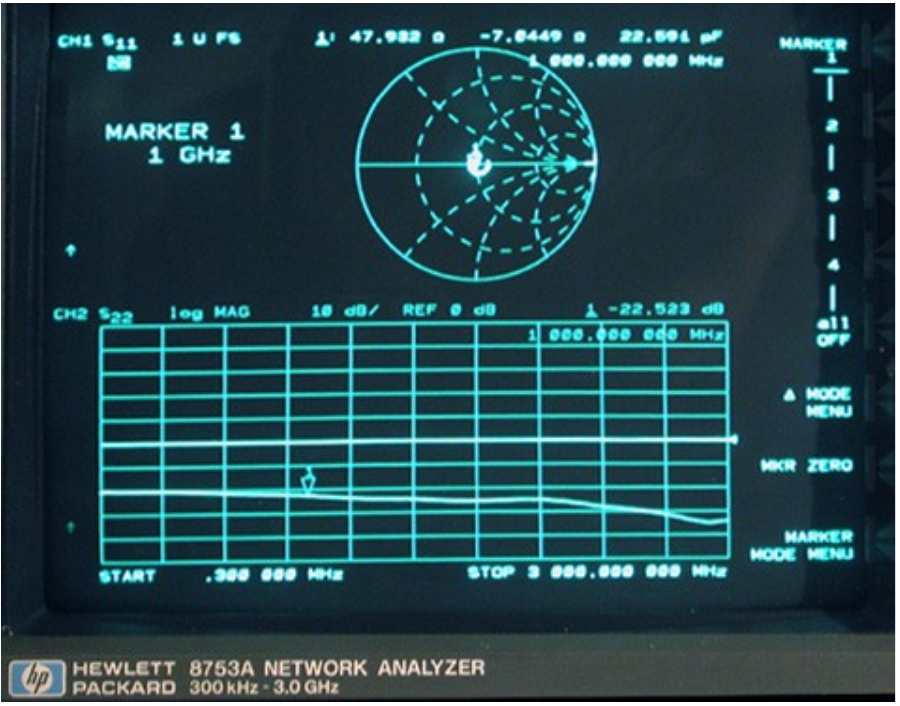
\includegraphics[width=0.6\linewidth]{images/network-analyzer-vector-graphics-display.png}
    \caption{A vector graphics display on a network analyzer\cite{assignment-text}.}
    \label{fig:vector-display-network-analyzer}
\end{figure}

\section{Vector Graphics - A Short Introduction}
Vector graphics expresses the contents of an image by using primitives, which are defined mathematically.
Primitives can be objects like lines (defined by their endpoints), squares (defined as a bounding box of two points) or curves (defined by the position of control points).
Special curves, called bézier curves, can be used to obtain complex, vectorized shapes.
The points are relative to the coordinate system of a 'scene', which is an abstract representation of an image.
Scenes are not tied to any specific physical screen resolution, but can be scaled to fit any resolution without loss of detail.

The major advantages of vector graphics are expressiveness and scalability.
Modern computing devices come in many sizes and aspect ratios.
With raster based solutions, graphics have to be regenerated for each new display size.
A vector based solution is inherently resolution independent, allowing for asset reuse across devices.

More information about vector and raster graphics is found in chapter \ref{chp:background}.

\section{Requirements}
\label{sec:requirements}
The group decided on a set of functional requirements based on initial research, listed in table \ref{tbl:func_req}.
Non-functional requirements given in the assignment text are listed in list \ref{lst:non_func_req}.

\begin{table}[h!]
\resizebox{\textwidth}{!}{
    \begin{tabular}{|l|l|}
        \hline
        \textbf{Requirement}                                                    & \textbf{Priority} \\ \hline
        The system should be able to produce and process vector primitives      & High     \\ \hline
        The system should display primitives on an vector display               & High     \\ \hline
        The system should support both straight lines and general bézier curves & High     \\ \hline
        The processor should be general                                         & High     \\ \hline
        The system should support modification of primitives                    & Medium   \\ \hline
        The system should rasterize primitives and support HDMI as an output    & Medium   \\ \hline
        A toolchain supporting the system should be available                   & Low      \\ \hline
    \end{tabular}
}
    \caption{Functional requirements.}
    \label{tbl:func_req}
\end{table}


\begin{table}[h!]
\resizebox{\textwidth}{!}{
    \begin{tabular}{|l|l|}
     	\hline															    	
        \textbf{Requirement}    												& \textbf{Priority} \\ \hline
        The processor should be implemented on a Xilinx FPGA								& High 	\\ \hline
        The unit must utilize a Silicon Labs EFM32 microcontroller to act as an				& High 	\\ 
        I/O processor 																		&   	\\ \hline
        The budget of 10 000 NOK should cover components and PCB production					& High 	\\ \hline
    
    \end{tabular}
}
    \caption{Non-functional requirements.}
    \label{tbl:non_func_req}
\end{table}


\section{A Vector Graphics Computer Architecture}

\begin{figure}[H]
    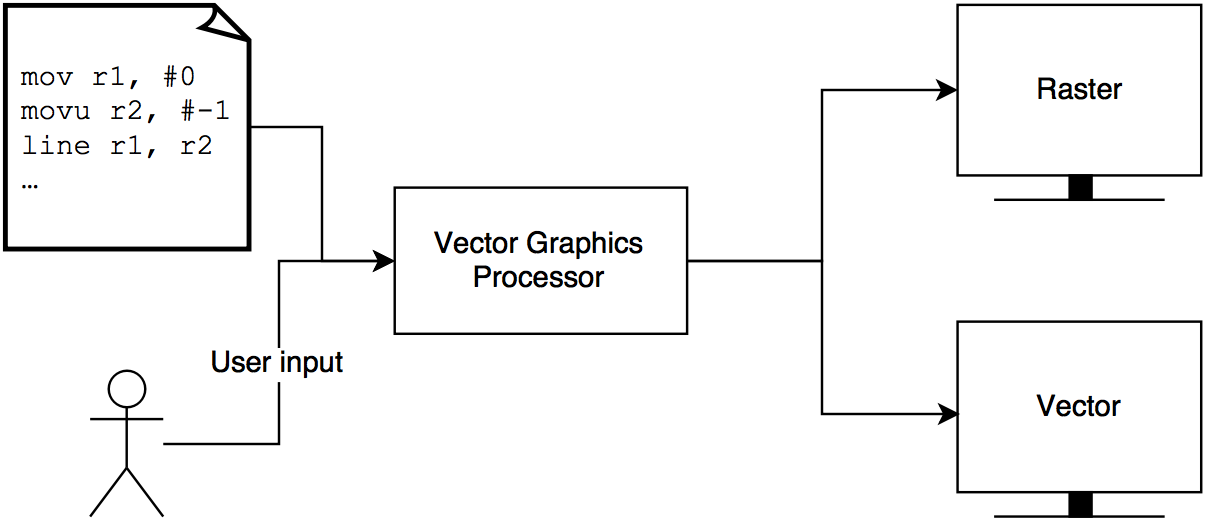
\includegraphics[width=\linewidth]{images/high_level_io.png}
    \caption{I/O overview.}
    \label{fig:io-overview}
\end{figure}

Based on the requirements, the group chose to make a general purpose computer with support for producing and processing vector graphics.
The computer would read instructions from memory, execute them on a processor core and render vector based scenes to different outputs.
To showcase the nature of vector graphics, a vector display in the form of an oscilloscope was chosen as the primary output device.
HDMI was included as secondary output to a raster display.
As a whole, the system should be assembled on a custom PCB, with the microcontroller serving as an I/O-unit while the main processor architecture and output-modules should be implemented on the \gls{fpga}.

\section{Lab Environment}
The NTNU Computer Design Lab was used frequently for this project.
The lab contains a wide variety of oscillators, signal generators and logic analyzers, which was used to test different parts of the system.
The lab also contains soldering equipment and aids - which was used extensively by the team when soldering the PCB - as well as loads of assorted electronic components.

A second lab at NTNU, ITV-458, was used by the team when programming the solution.
The lab contains computers running Ubuntu and tools for working with FPGAs.

\section{About this report}
This report is meant to give a thorough understanding of the system designed by the group.
Having introduced the assignment and described a very abstracted architecture, the next chapters introduces the system created by the group as well as give some background on computer graphics and a theoretical overview of vector graphics.

Part two presents the designed architecture in detail, outlines the programming model and elaborates on the implementation of specific subparts of the system.

Finally, part three presents performed tests, results, discussion and a conclusion.

\section{Conventions}
// TODO: Describe any conventions used in the report.
This report should be read with the following considerations in mind:

\begin{description}
    \item[group and team] 'The group' refers to everyone working on this project. The main work loads (System architecture, I/O and PCB design), were split among smaller teams. 'The team' refers to the team responsible for this functionality.
\end{description}

\chapter{\vthreek}

\begin{figure}[H]
    \centering \includegraphics[width=0.7\linewidth]{images/board_angle.jpg}
    \caption{\vthreek}
    \label{fig:board-angle}
\end{figure}

The end result of the group's work on this project is a computer architecture made with the defined requirements in mind.
The architecture is named V.E.C.T.O.R. -3000, an acronym for Very Efficient Computer for Transferring graphics to Oscilloscope and Raster screens, with the -3000 added as an homage to the retrofuturistic associations of vector graphics in popular culture.

\vthreek is a general purpose vector graphics processor, capable of processing and producing vector graphics. 
It utilizes a multi cycle processor core, a technique that benefits the processor by allowing shorter clock cycles.
This feature, together with the minimalistic \gls{isa} inspired by \gls{risc}\cite{risc} and \gls{mips}\cite{mips}, results in a computer that fits into today's computing world.
The output is sent to the oscilloscope, where it is displayed on the vector display in it's full glory.

While the system developed is still only a prototype, it demonstrates the capabilities of modern processors when applied to vector graphics. 




\chapter{Background and Theory}

Vector graphics have been popular in the computer industry for many years, seeing frequent use in analogue oscilloscopes, video arcade games \cite{astroids}, and as display devices for computers \cite{ibm2250}.

\section{Vector Graphics}

With vector graphics, mathematical expressions are used to describe an image.
The image, or the scene, is made up of primitives that describe paths and curves in order to create more complex shapes.

Vector graphics are predominantly used in 2D graphics, and is called vector graphics in order to distinguish from 2D raster graphics. In 3D graphics the internal representation of the world is usually described with vector primitives (points that form triangle surfaces for example). TODO: Some citation.

Some computer font types, like TrueType uses vector graphics and more specifically Bézier curves to represent glyphs\cite{truetype}.


TODO: Make coherent.


\section{Vector Monitor}
A vector display or monitor, is a device that draws graphics from point to point. A vector monitor utilizes CRT (Cathode Ray Tube) technology, which contain one or more electron guns and a phosphorescent screen to view images. The electron beam is deflected horizontally and vertically using electrostatic deflection. \cite{vector-monitor}

Unlike the CRT raster displays (old television sets or computer monitors), a vector monitor does not scan repeatedly in a fixed pattern. Instead it draws a point based on two voltages, one for horizontal placement and one for vertical.

One of the major advantages with vector monitors is that, since they are able to draw directly from one point to another, they do not suffer from artefacts like aliasing and pixelation. The drawback however is its inability to fill shapes in an efficient way. Therefore, vector monitors usually only draw the outline of shapes.


\section{Drawing to a oscilloscope}
As vector monitors are no longer a easily available, we need an alternative method of displaying vector graphics. It is possible to modify a CRT monitor, so that it one can manually control the deflectors, but this is quite cumbersome. The other method is using an oscilloscope, which gives an easy interface to these deflectors. This section will explain how to use the oscilloscope as a vector monitor.


To be able to draw to a oscilloscope, the oscilloscope must support at least two input channels, and the ability to draw in X-Y mode. In X-Y mode, two of the input channels (usually Ch1 and Ch2) governs the electron ray deflectors. If the channels are provided a constant voltage, a dot will be displayed on the screen, in contrast to normal mode, where  a line would be drawn.

The voltage on channel 1 will normally decide the beam's horizontal position, and channel two, its vertical position. To draw a line on the oscilloscope, one would need to repeatedly change the voltage of one or both channels back and forth.  Changing the voltage on only one channel will produce a horizontal or vertical line. 



% Part II
\part{Solution}
\chapter{System Overview}

\section{Architectual structure}

\begin{figure}[h!]
    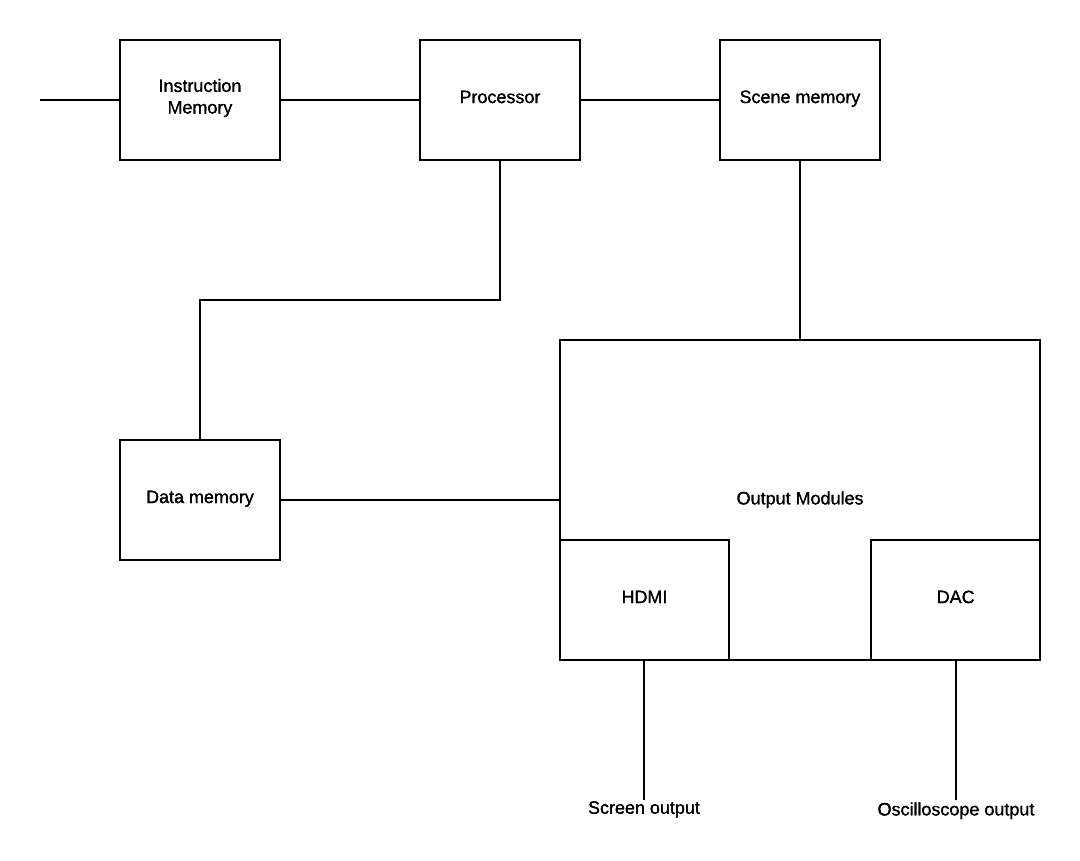
\includegraphics[width=\linewidth]{images/system-overview.png}
    \caption{A logical overview of the \vthreek architecture}
    \label{fig:system-overview}
\end{figure}

Figure \ref{fig:system-overview} shows how the major building blocks of the \vthreek architecture come together on a conceptual level.
Separation of instruction and data memory makes it a Harvard-like architecture.
The processor reads from instruction memory, executes instructions and adds/updates vector primitives in the scene memory.
Preprocessing these primitives for output is done by the output modules.
For the HDMI output, this involves rasterizing each primitive and maintaining a framebuffer.
The oscilloscope output is generated by serializing primitives onto two DACs.

\section{Programming Model}

The \vthreek architecture is fairly conventional and largely RISC-inspired.
This makes its programming model fairly similar to that of other modern computers.

A .v3k program is assembled on a host machine, transferred to the microcontroller which in turn loads it into instruction memory.
As previously mentioned, the \vthreek architecture is general, and as such, offers support for integer arithmetic, load/store instructions and simple branching.
Additionally, instructions for adding and processing vector primitives such as lines and curves are available.
A complete description of the \vthreek ISA is available in appendix \ref{app:ISA}.

\subsection{A Simple \vthreek Program}

\begin{lstlisting}[label=lst:simple-program]
mov r1, #0
lsl r1, r1, #16
mov r1, #0

mov r2, #65535
lsl r2, #16
mov r2, #65535

line r1, r2
strp #0x00000001
\end{lstlisting}

Listing \ref{lst:simple-program} shows a very simple \vthreek program.
It simply draws a line across the scene, from bottom left corner to top right.

Vector primitives consist of a varying number of integer numbers.
In the case of a line, it consists of four 16-bit coordinates.
To utilize registers effectively, each 32-bit register is loaded with one x,y coordinate-pair.

The first three lines put the coordinates $0,0$ in register \texttt{r1}, the next three puts $65535$ in register \texttt{r2}.
The values in the registers are then used to create a line starting at \texttt{r1} and ending at \texttt{r2}.
Finally, the line is written to the scene memory using \texttt{strp}.

\chapter{Processor Core}

Chapter \ref{chp:system-overview} describes how vector graphics are supported and integrated into the \vthreek architecture.
This chapter elaborates on how the processor core is designed, focusing especially on features directly related to vector graphics.

\section{The \vthreek processor}

The processor core is the main processing and control unit in the \vthreek architecture.
As depicted in figure \ref{fig:system-overview}, the processor core reads instructions from the instruction memory, and writes/reads data to/from the data and scene memories.
The processor core is designed as a multi-cycle, MIPS-inspired processor with features added to support processing of vector graphics.
When planning which features to include and which techniques to utilize, the group considered features like pipelining and even multicore designs to improve performance.
In the end, the decision was made to make the initial design simple, but keep efficiency and performance in mind.

\begin{figure}[H]
    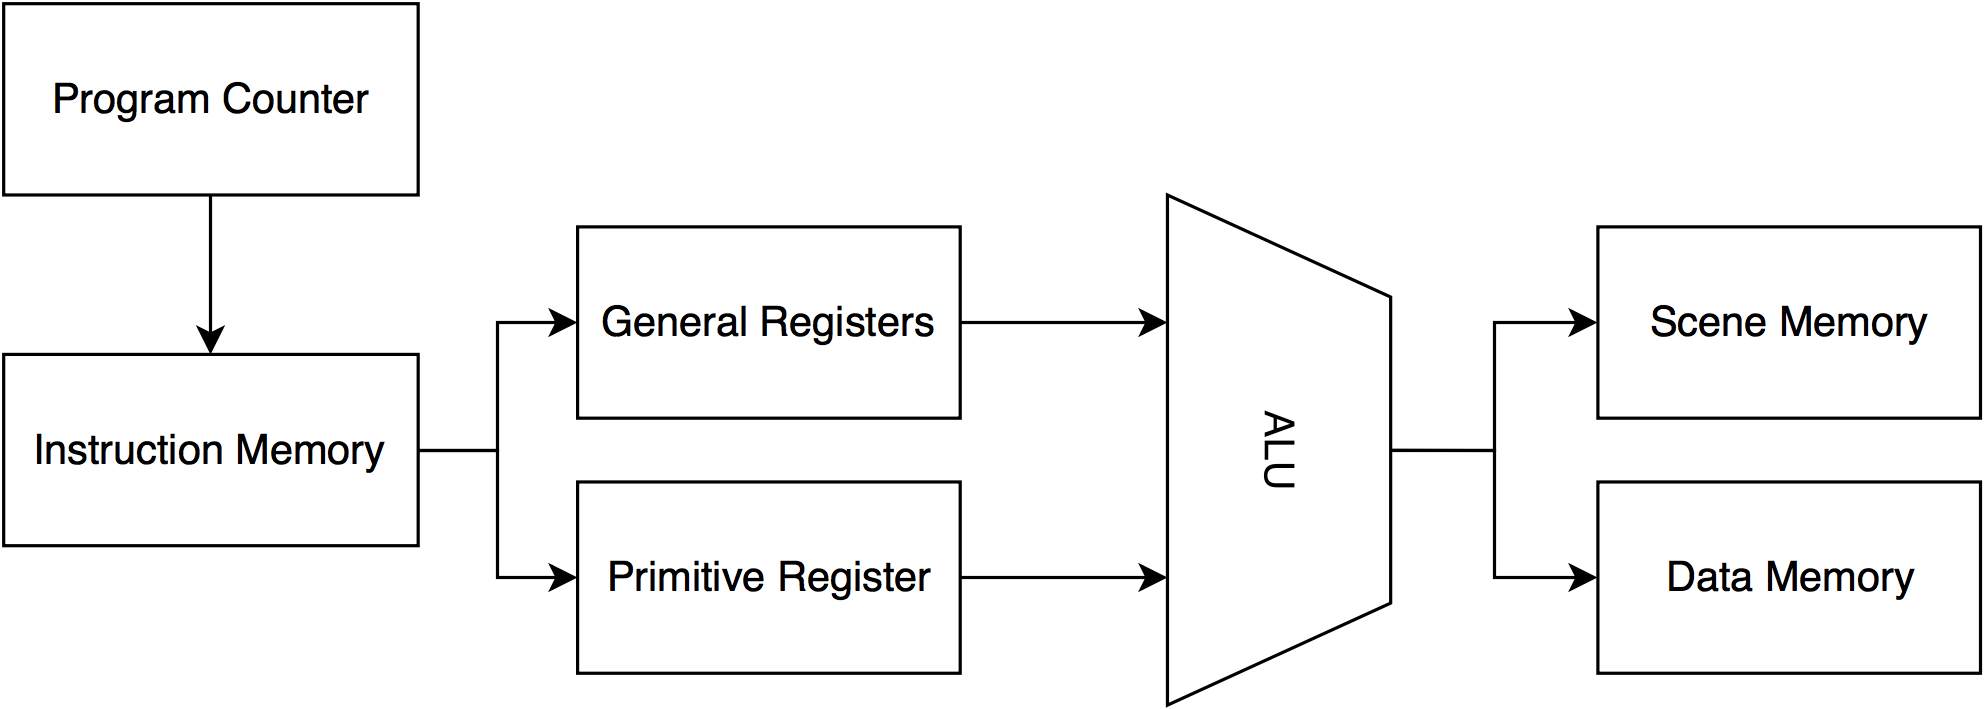
\includegraphics[width=\linewidth]{images/core-components.png}
    \caption{Overview of the main components in the processor core.}
    \label{fig:core-components}
\end{figure}

Figure \ref{fig:core-components} shows how data flows through the subcomponents of the processor core.
In addition to the components in the figure, the core includes a control unit.
Each component is described in detail in their respective section below, the following is a short introduction to their responsibilities.

\begin{description}
    \item[Program counter] \hfill \\
        The program counter keeps track of the address of the next instruction to be executed.
        Depending on the instruction currently being executed, the program counter is either incremented or overwritten.
    \item[Control] \hfill \\
        The control unit keeps track of the state of the processor, namely fetch, execute and stall, and issues the appropriate control signals to the other components.
    \item[Register] \hfill \\
        The register bank is the short term memory of the core, feeding operands to the ALU, and recieving data which may be stored based on the control signals.
    \item[ALU] \hfill \\
        The ALU performs operations on the data it receives from the register unit and outputs the result.
    \item[Primitive Register] \hfill \\
        The primitive register is a special purpose register, containing the vector primitive that the core is currently processing.
\end{description}

\section{Instruction Format}

Instructions in the \vthreek architecture are 32 bits wide.
As opposed to the MIPS architecture, they can't all be grouped into categories based on their format.
They do however share some common traits.
All instructions start with a 6-bit opcode, a unique identifier for each instruction.
The remaining bits are used either to address registers, to encode immediate values or as a combination.
Some instructions also have don't care bits, parts of the instruction that can be either 1 or 0 without influencing the outcome of execution.
For instructions that address one or more registers, a general convention of using the five bits directly after the opcode for the destination register and addressing source registers in successive five bit chunks.
Figure \ref{fig:instruction-format} shows how various parts of an instruction word is utilized.

\begin{figure}[h!]
    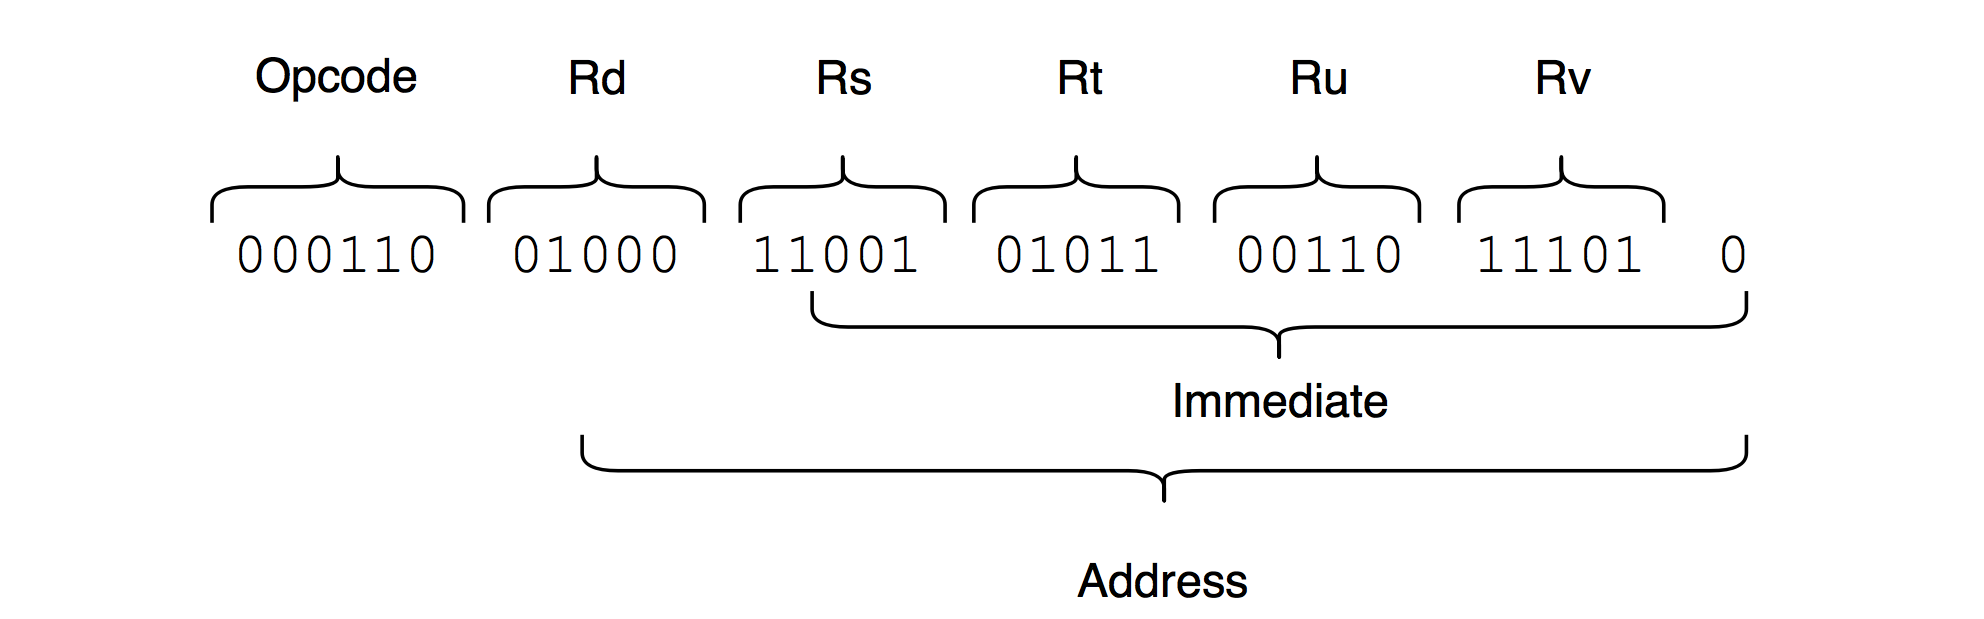
\includegraphics[width=\linewidth]{images/instruction-format.png}
    \caption{\vthreek instruction format.}
    \label{fig:instruction-format}
\end{figure}

As an example, the \texttt{jmp} instruction is encoded with the opcode \texttt{000001}, seven don't care bits followed by the 19-bit jump target.
The \texttt{bezcube} instruction initializes a cubic Bézier primitive into the primitive register, reading the coordinates of the four control points from four general purpose registers.
With 32 general purpose registers, five bits are needed to address them.
That means that the \texttt{bezcube} instruction is encoded with its six bit opcode, \texttt{000111}, followed by five don't care bits, then four 5-bit chunks, one for each register.
The final bit is also don't care.

\section{Data Path}

\begin{figure}[h!]
    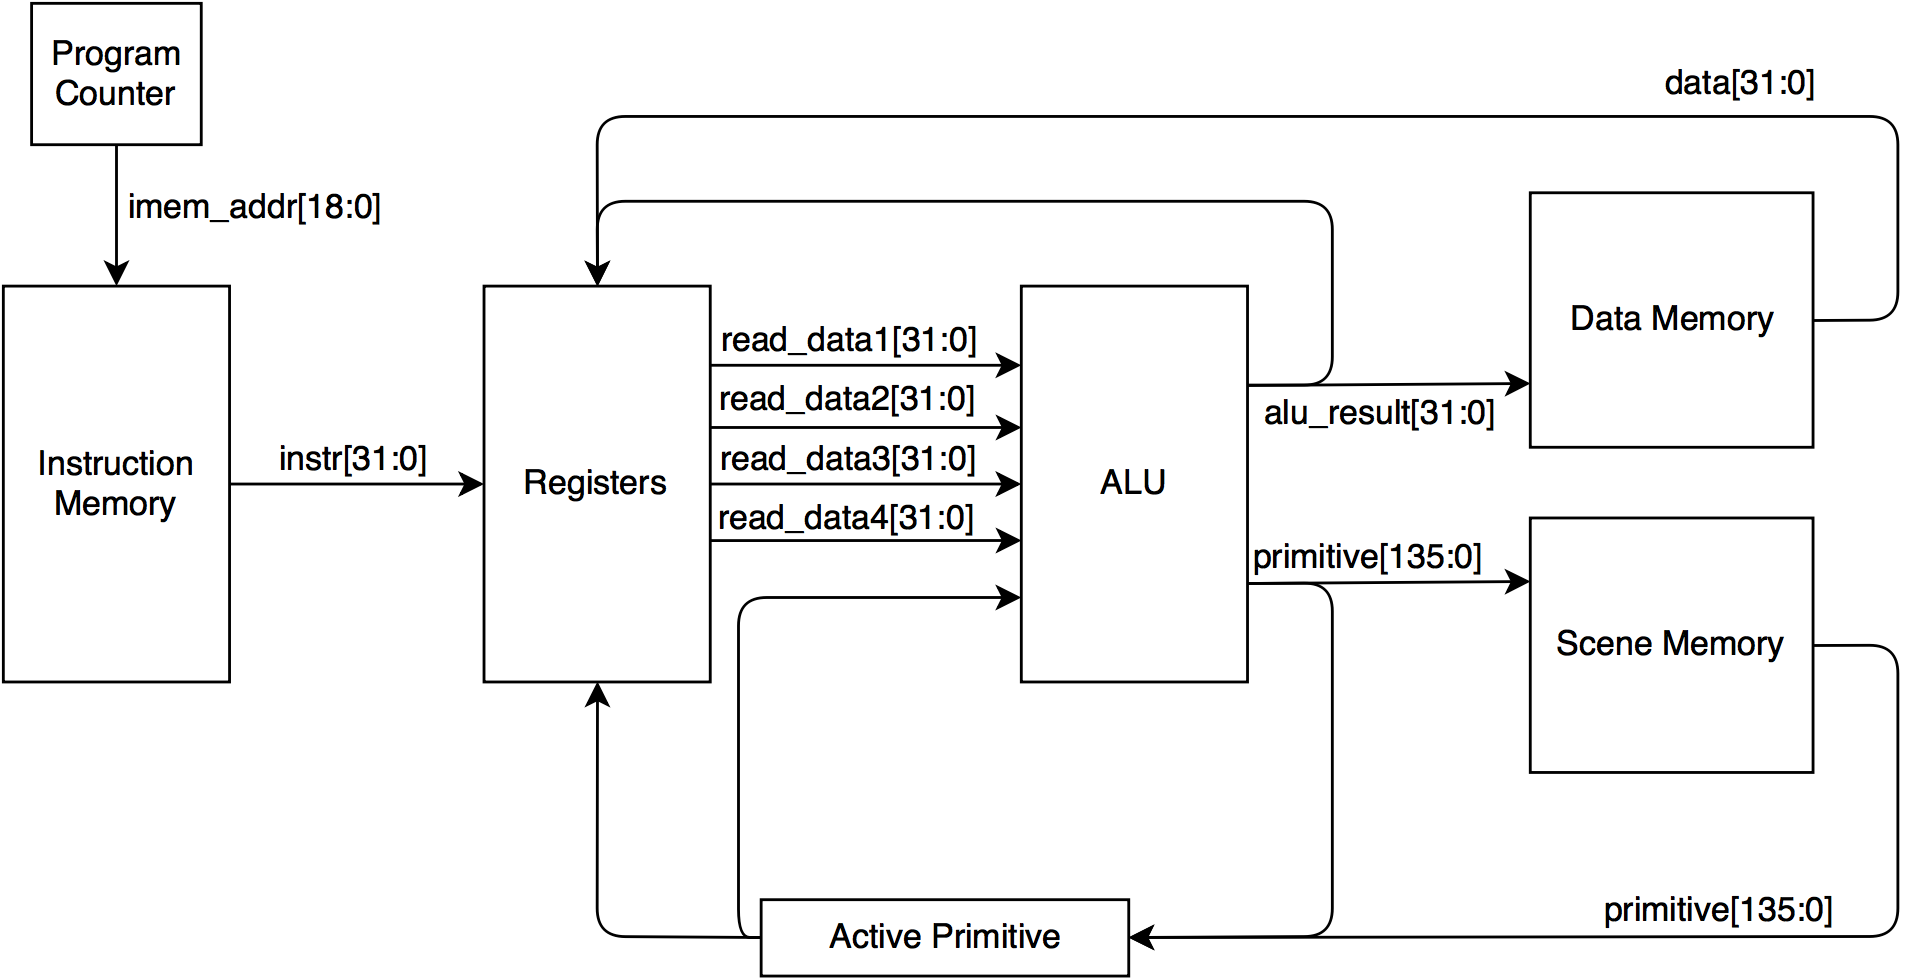
\includegraphics[width=\linewidth]{images/Data_path.png}
    \caption{RTL sketch of the data path.}
    \label{fig:datapath}
\end{figure}

The data path of the \vthreek architecture consists of a registerfile encapsulating the 32 general purpose registers, a separate, special purpose, 136-bit vector primitive register, a functional unit, the ALU, and instruction, scene and data memories.
To explain how these work together, each component will be explained in the order with which an instruction being executed interacts with them.

\subsection{Instruction Memory}

\begin{figure}[h!]
    \centering
    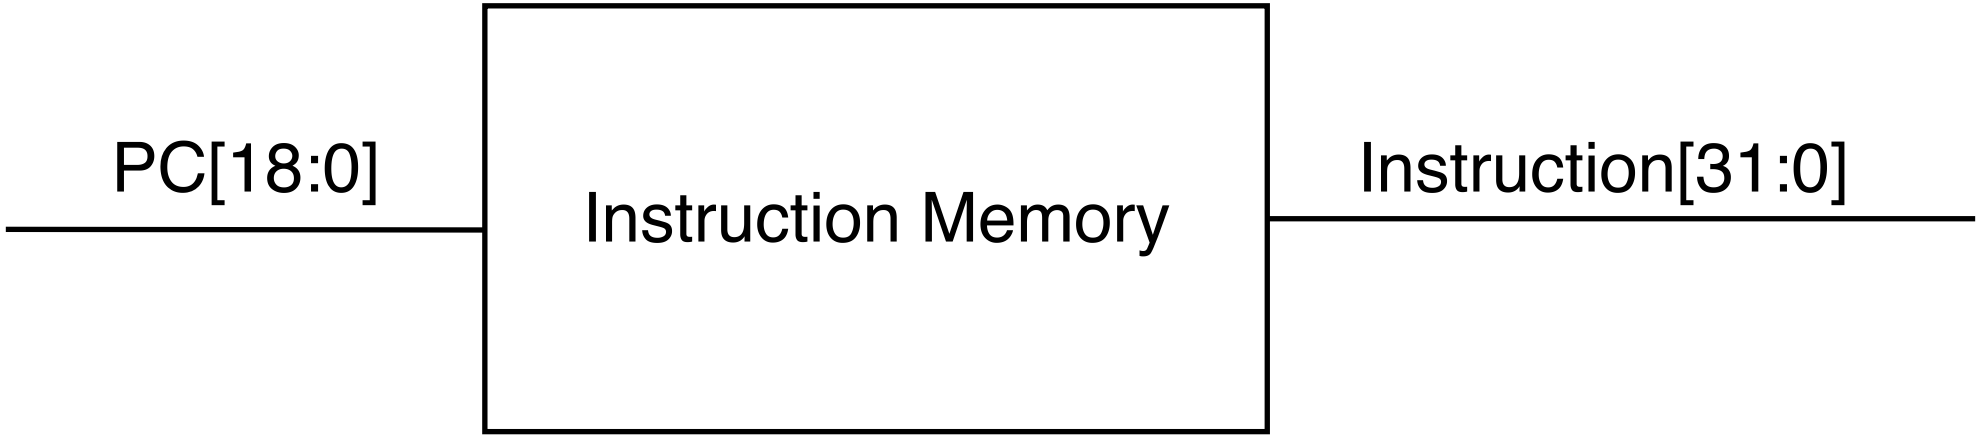
\includegraphics[width=0.6\linewidth]{images/instruction-memory.png}
    \caption{I/O for the instruction memory.}
    \label{fig:instruction-memory}
\end{figure}

Figure \ref{fig:instruction-memory} shows the signals going into and coming out of the instruction memory.
The program counter value is the address of the desired instruction.
Due to only being able to read 16 bits at a time from the SRAM, the group implemented a stateful instruction fetch module encapsulating the instruction memory.

\subsection{Registers}

\begin{figure}[h!]
    \centering
    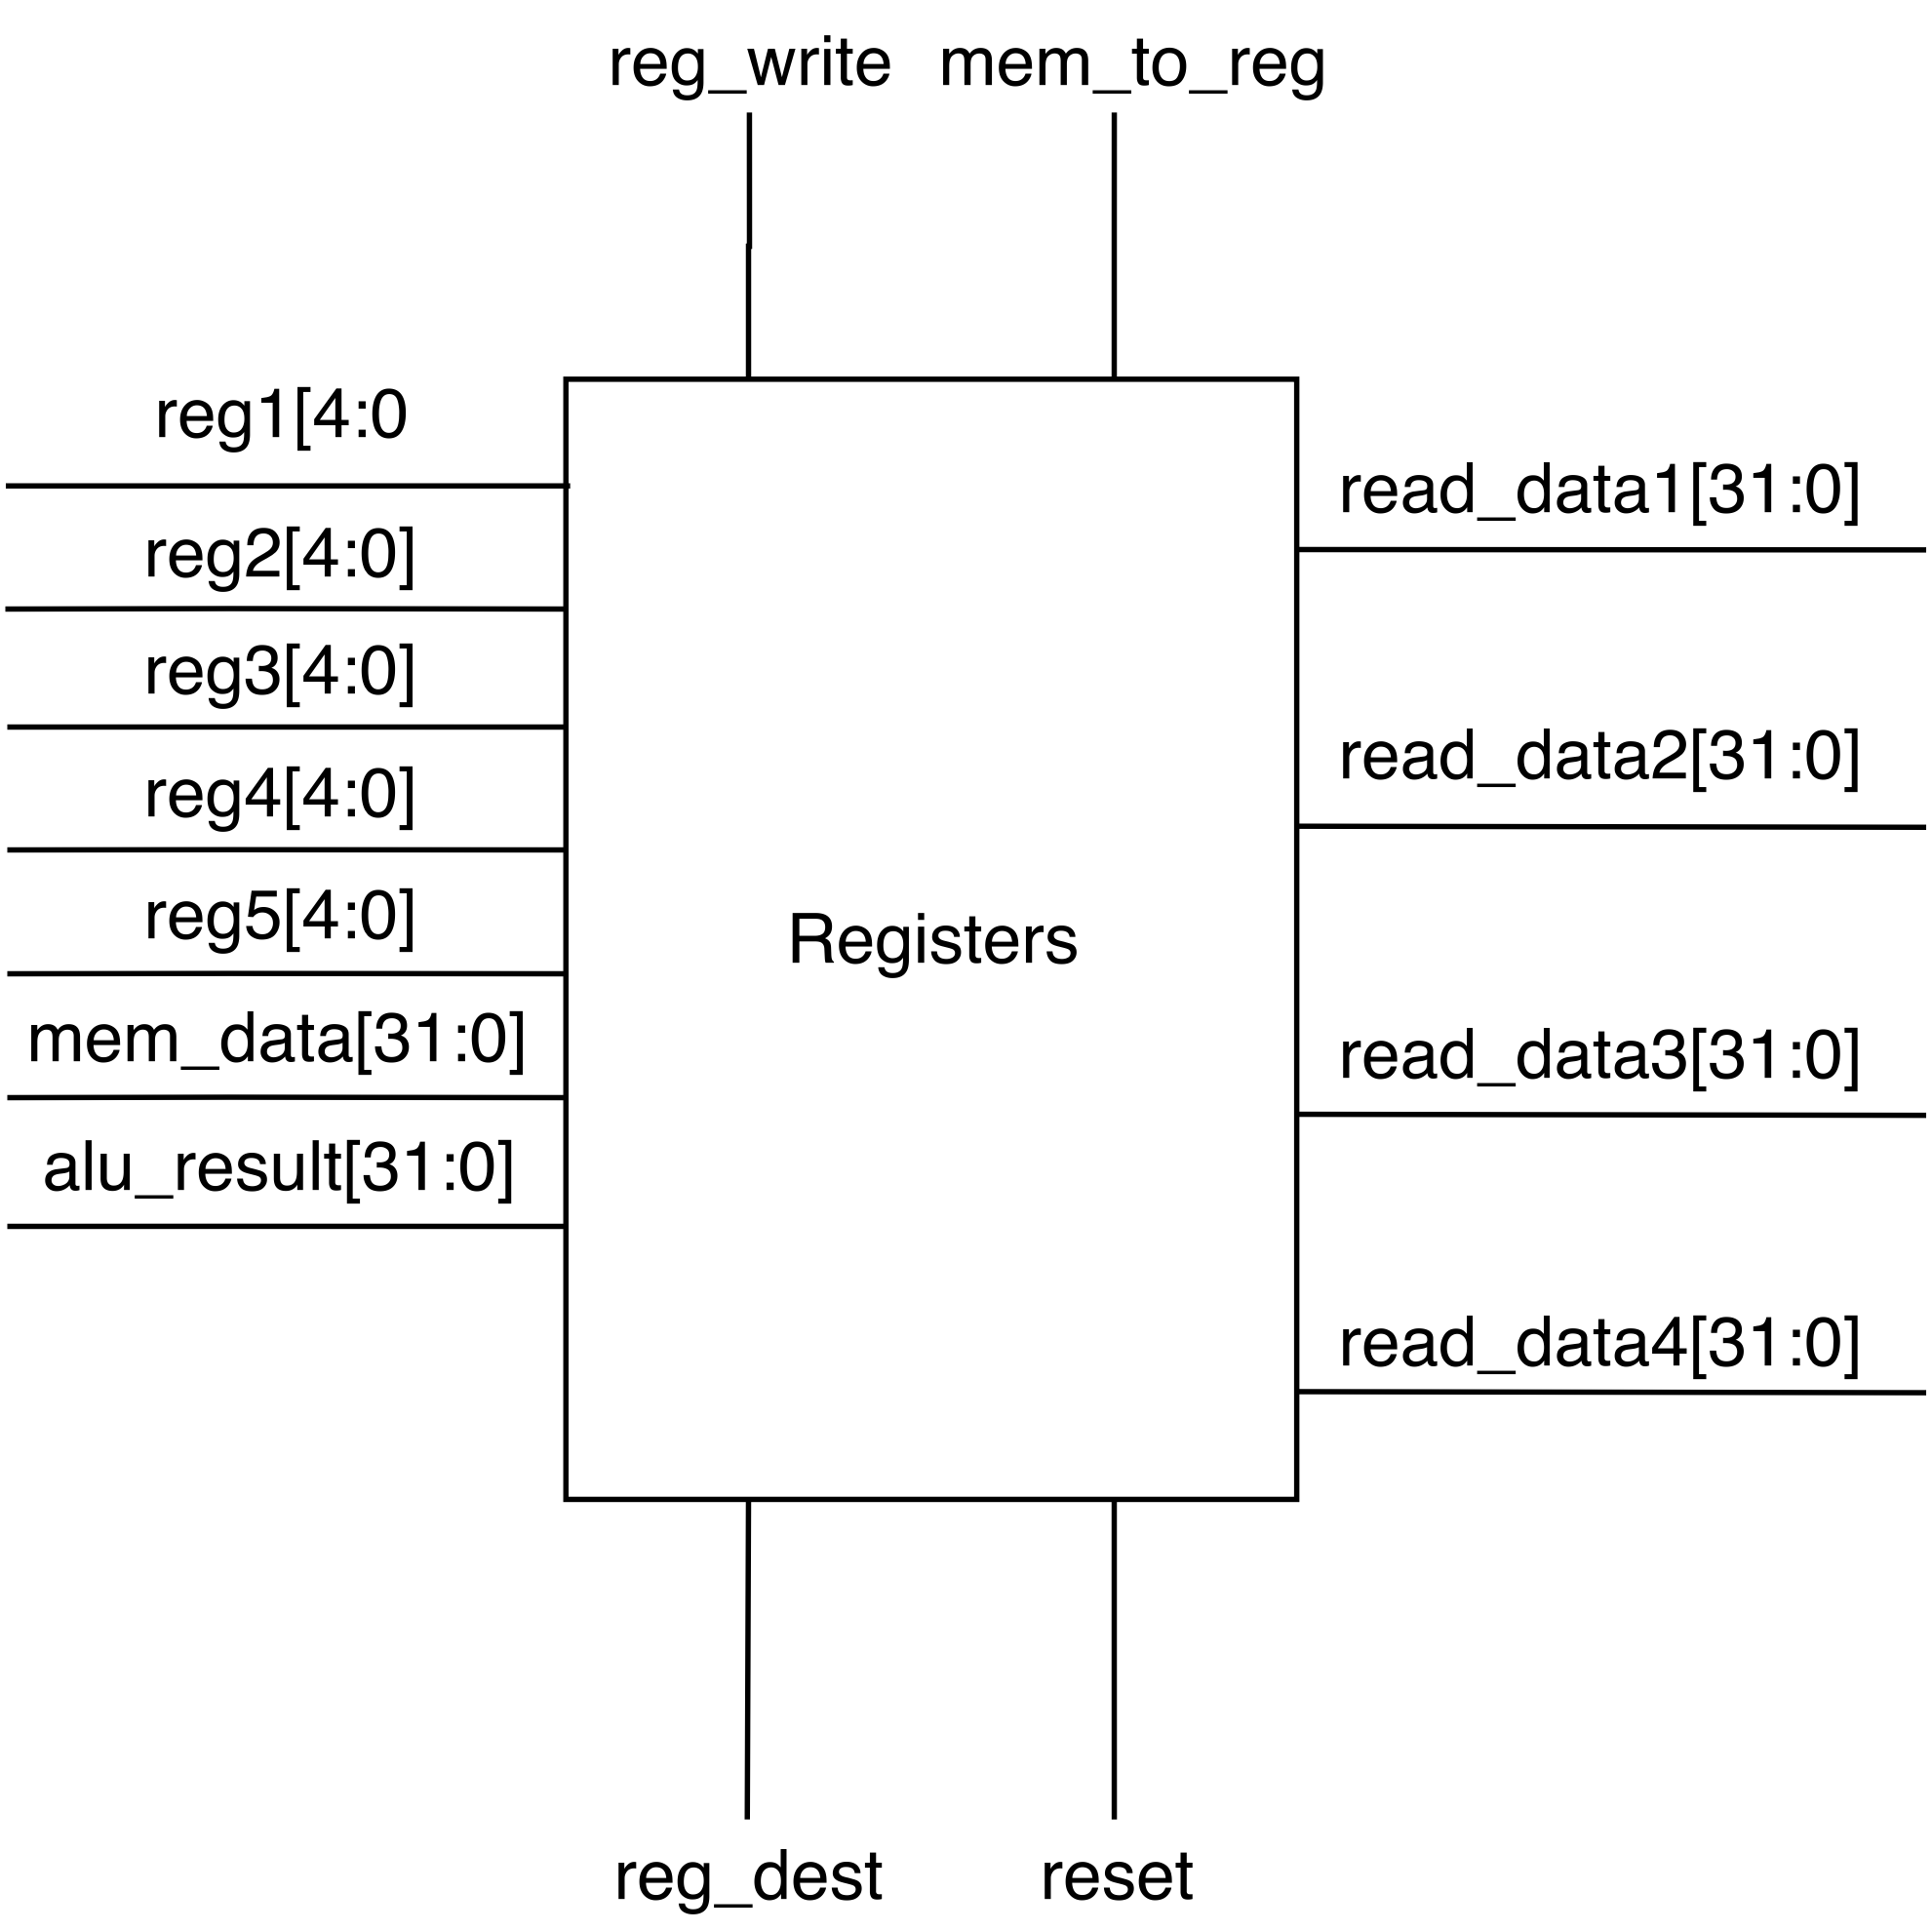
\includegraphics[width=0.6\linewidth]{images/registers.png}
    \caption{I/O for the register module.}
    \label{fig:registers}
\end{figure}

After being read from the instruction memory, an instruction is decoded and wired as input to the register module.

The \vthreek architecture provides 32 32-bit general purpose registers.
These are organised into a registerfile.
As can be seen in Figure \ref{fig:registers}, this module receives five register addresses.
The values in the addressed registers are continuously output on the \texttt{read\_data} signals.
32-bit input values are taken as input from the ALU and the data memory, to potentially be written to into a register.
There are four control signals, \texttt{reset, mem\_to\_reg, reg\_dest} and \texttt{reg\_write}.
\texttt{reset} signals the module to clear all registers of their contents.
\texttt{reg\_write} signals wether or not data should be written in the current cycle.
\texttt{reg\_dest} indicates which of the \texttt{regX} registers should be used as the destination register.
Similarily, \texttt{mem\_to\_reg} indicates wether the data from memory or the alu result should be written.

The special purpose primitive register functions in much the same way, only with a single register.
Its inputs, outputs and control signals can be seen in Figure \ref{fig:primitive-register}.
Since there is only one register to address, the primitive register doesn't take any part of the instruction as input, but rather outputs its current value continuously.
Control signals only determine wether or not the register contents should be overwritten and if yes, what data source should be used to overwrite.

\begin{figure}[h!]
    \centering
    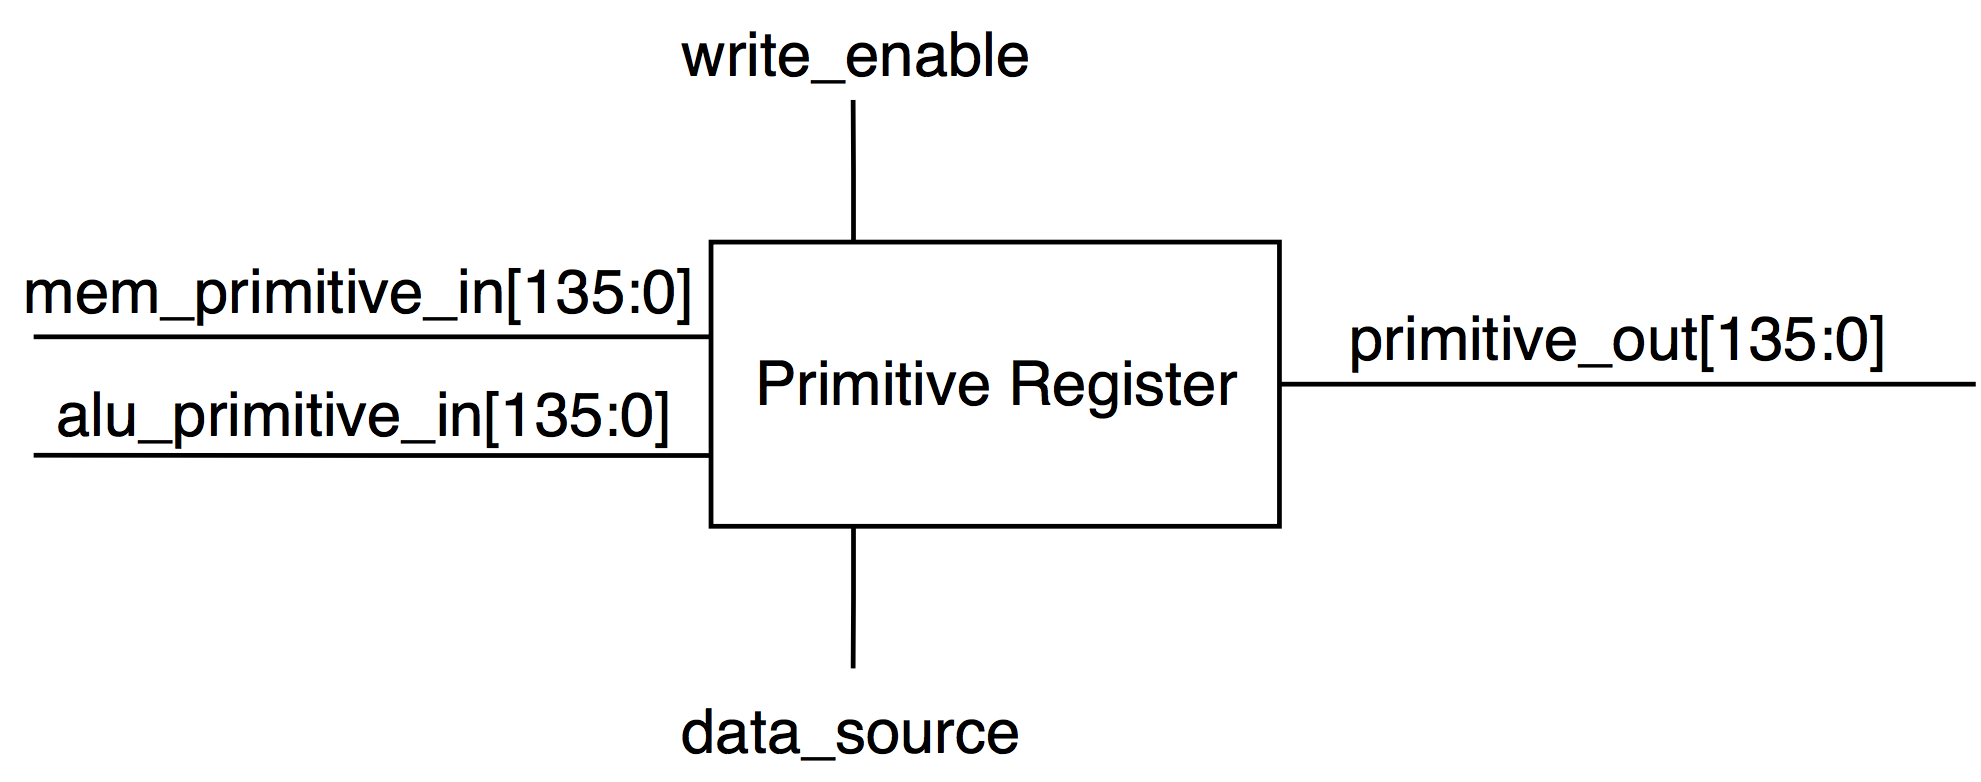
\includegraphics[width=0.6\linewidth]{images/primitive-register.png}
    \caption{I/O for the primitive register.}
    \label{fig:primitive-register}
\end{figure}

\subsection{ALU}

\begin{figure}[h!]
    \centering
    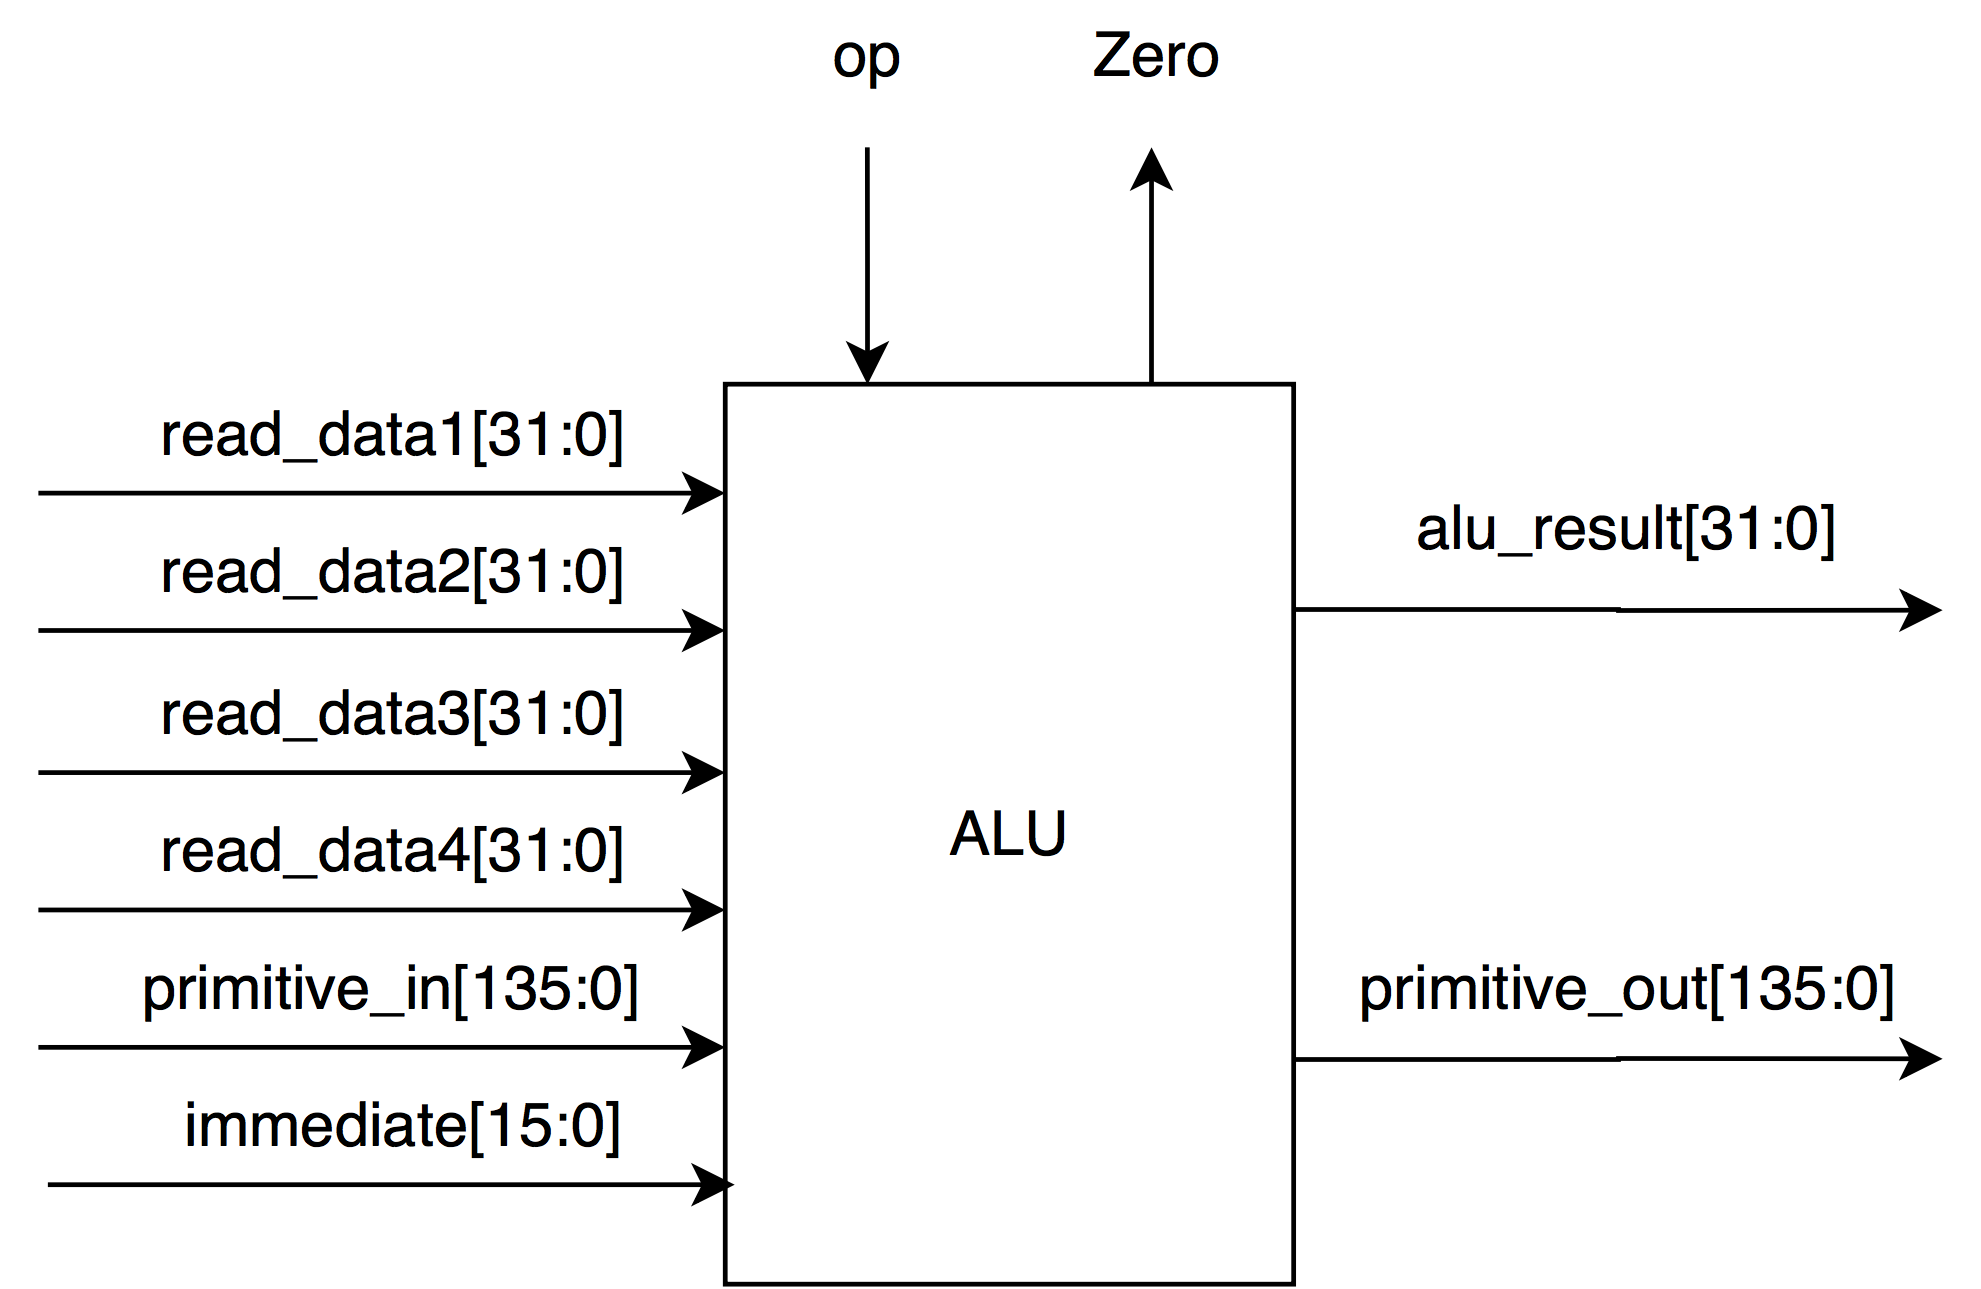
\includegraphics[width=0.8\linewidth]{images/ALU.png}
    \caption{I/O for the ALU.}
    \label{fig:ALU}
\end{figure}

The ALU is the main functional unit of the processor.
It is responsible for performing arithmetic and logical operations on operands from the registers.
Additionally, it supports a number of operations associated with vector primitives.
For the initialization instructions, \texttt{line}, \texttt{bezquad} and \texttt{bezcube}, coordinates read from the general purpose registers are assembled into primitives.
\texttt{getp\{1,2,3,4\}} and \texttt{setp\{1,2,3,4\}} work on individual parts of a primitive.

As shown in Figure \ref{fig:ALU}, the unit also receives an immediate value, taken straight from the decoded instruction, and a control signal, \texttt{op}, which determines the operation to be performed.

\subsection{Data and Scene Memories}

Scene and data memories have similar interfaces, see Figure \ref{fig:data-scene-memories}, the major exception being data width and size.
Data words in scene memory are 136 bits wide, with space for 1024 words.
To allow for the rather unusual word size as well as allowing both the processor core and the output module to interface with the scene memory simultaneously, the scene memory was instantiated as a block RAM on the FPGA.
Words in general data memory are 32 bits wide.
Their input address bus determines either which address to read from or write to.
The \texttt{write\_enable} control signal specifies whether a read or write should be performed.

\begin{figure}[h!]
    \centering
    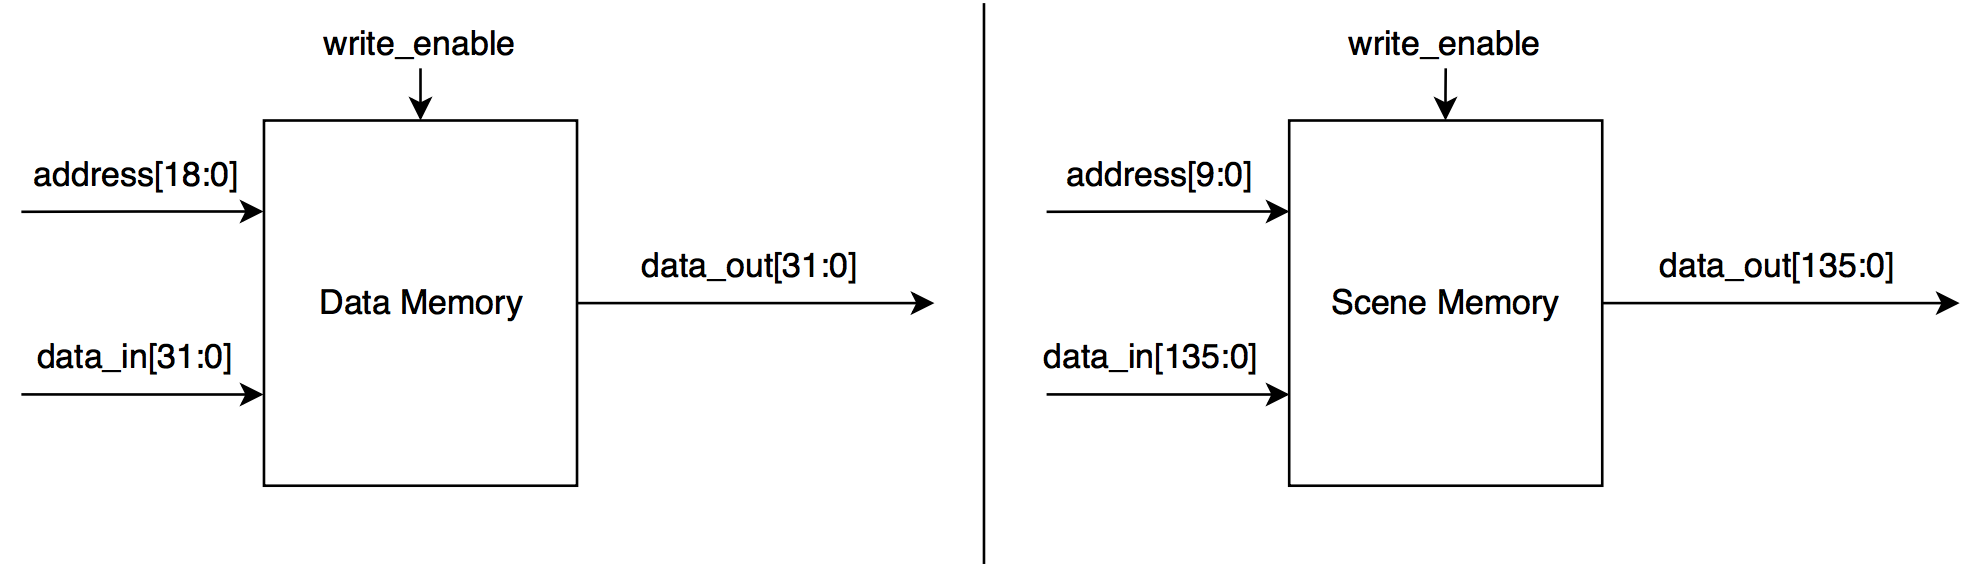
\includegraphics[width=0.8\linewidth]{images/data-scene-memories.png}
    \caption{I/O for data and scene memory modules.}
    \label{fig:data-scene-memories}
\end{figure}


\section{Control Path}

Having examined how instruction, data words and primitives move through the system, this section elaborates on the how the various components involved in the data path are controlled, and what determines their behavior.

Every time a new instruction is read, it is decoded and relevant parts fed into a control unit. 
Depending on the instruction, the unit sets its output control signals so that the modules they control behave as desired.
Figure \ref{fig:controlpath} shows how control signals are routed.
Table \ref{tbl:control-signals} lists all control signals and their functionalities.

The control unit maintains processor state.
Since the prototype implemented by the group is non-pipelined, a simple state machine with three states is sufficient.
These are fetch, execute and stall.
Figure \ref{fig:state-machine} shows the states and the conditions for transitioning between them.

While an instruction is being read, the processor is in the fetch state.
To avoid modifying data in registers or in memory, control signals are set to values that disable any writing operations.
In the execute state, control signals are determined by the instruction.
In the case of a stall, the control signals are maintained until the word to be loaded has been written into its destination.

The final functionality implemented in the control unit is a primitive counter.
All instructions that either add new or remove existing instructions in the scene memory cause the counter to be incremented or decremented respecively.
This signal is used in the output module.

\begin{figure}[h!]
    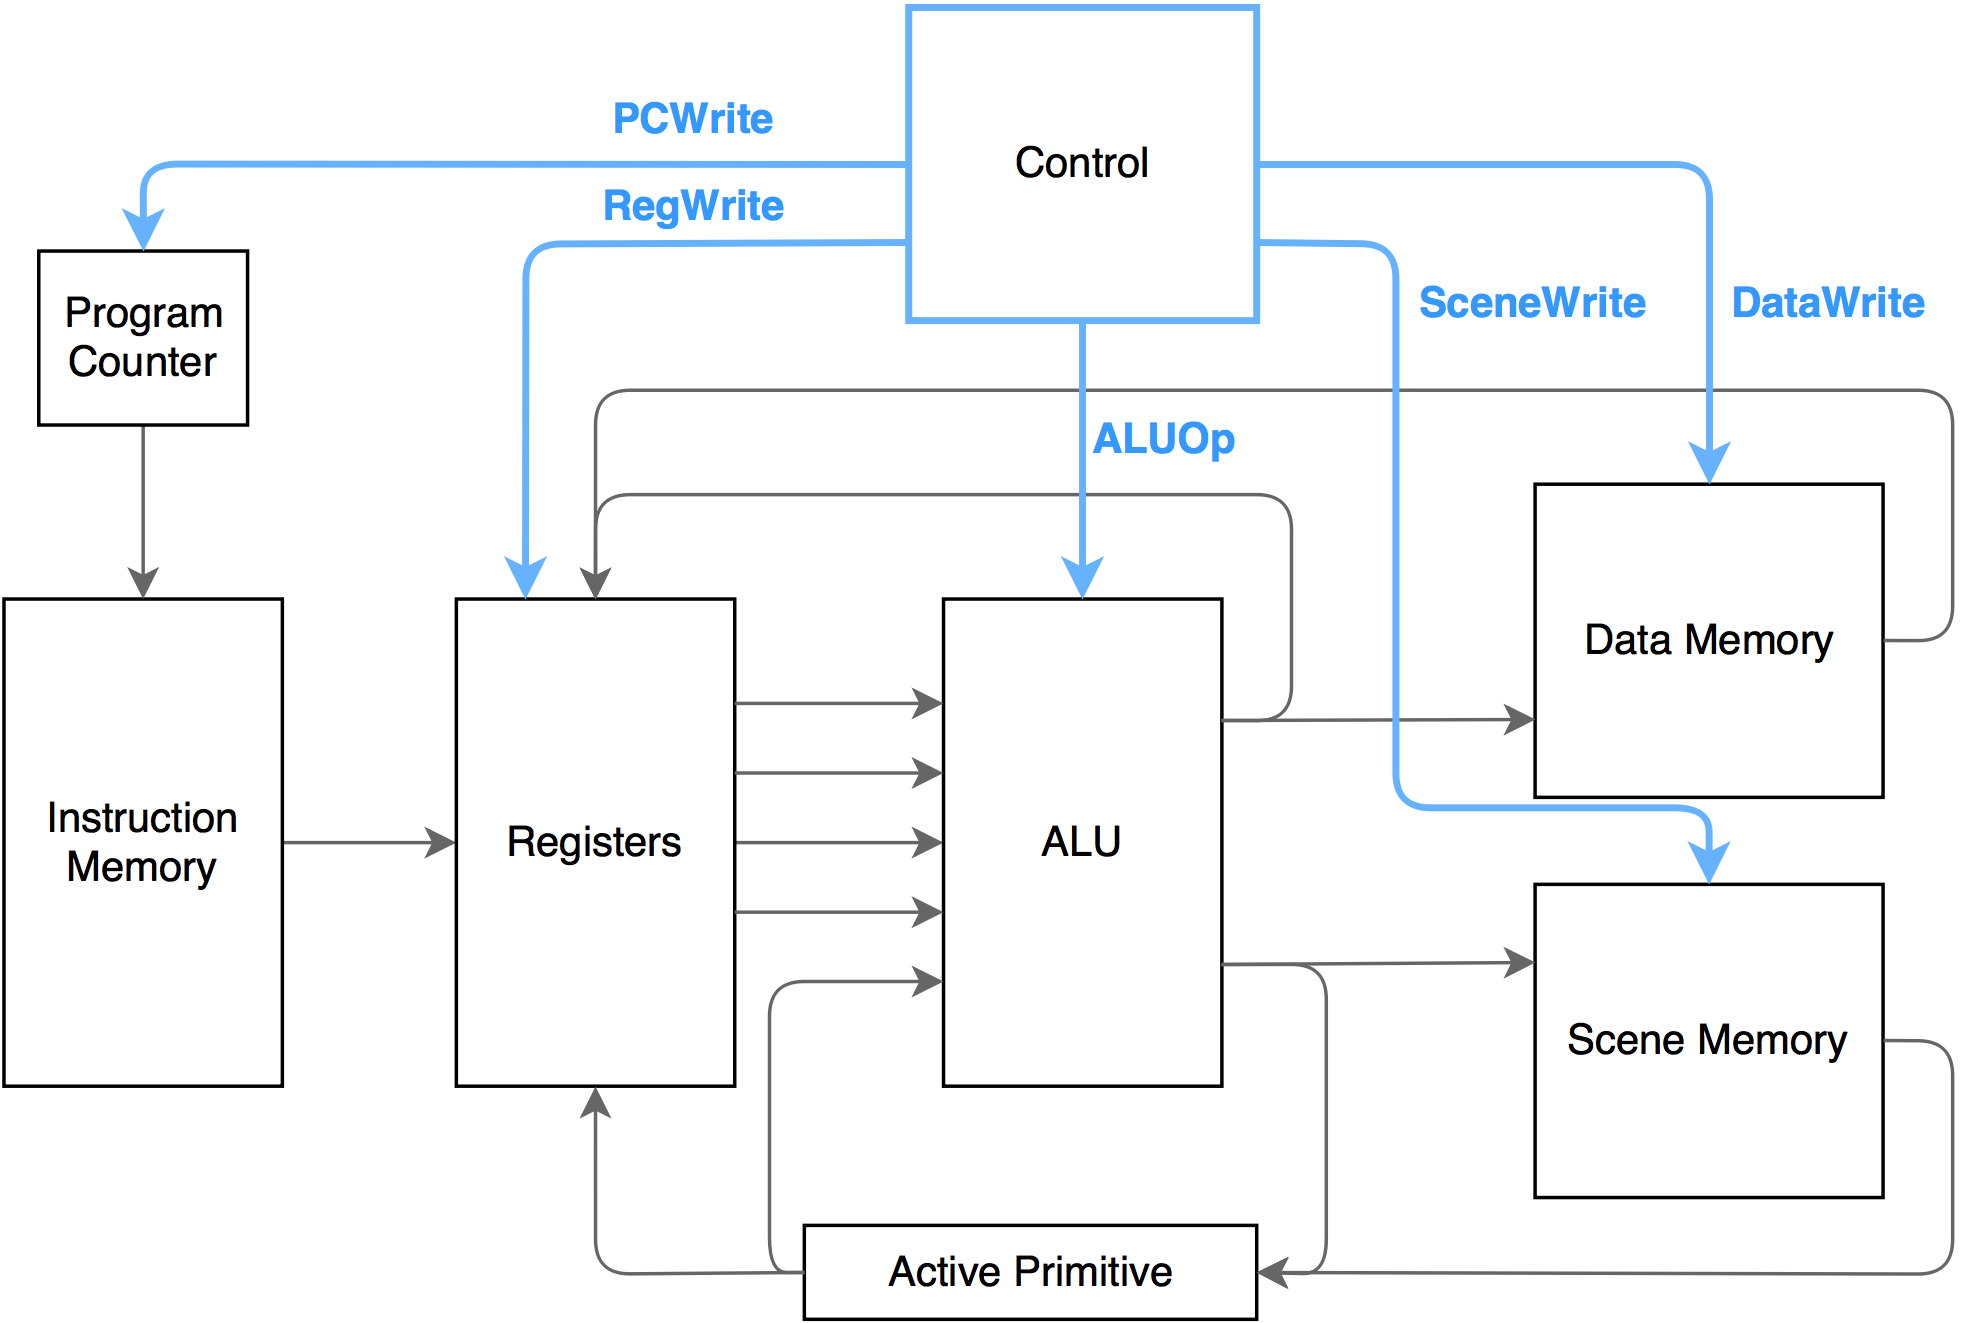
\includegraphics[width=\linewidth]{images/Control_signals.png}
    \caption{RTL sketch of the control path.}
    \label{fig:controlpath}
\end{figure}

\begin{figure}[h!]
    \centering
    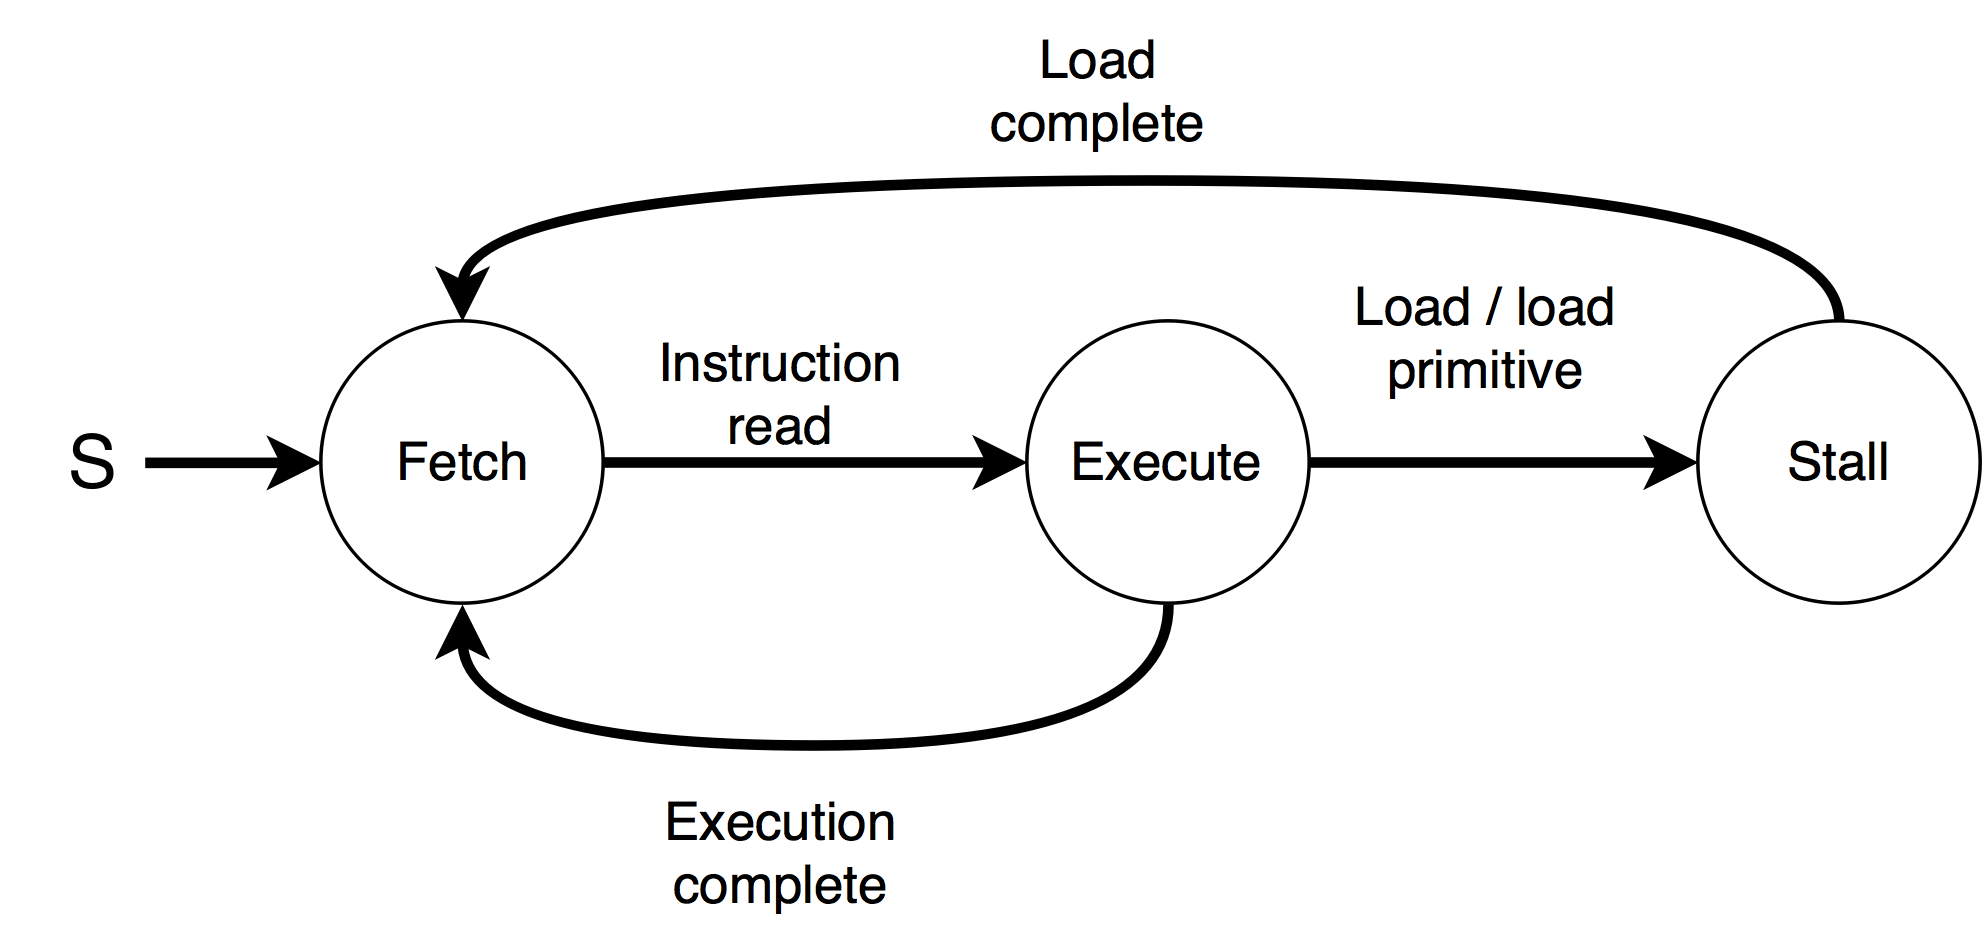
\includegraphics[width=0.6\linewidth]{images/state-machine.png}
    \caption{Processor core state machine.}
    \label{fig:state-machine}
\end{figure}

\begin{table}
    \begin{tabular}{|p{5cm}|p{7cm}|}
        \hline
        Signal             & Description                                                                                                                 \\ \hline
        \texttt{reg\_dest}          & Signalizes which register register address from the instruction to use as a destination register.                           \\ \hline
        \texttt{reg\_write}         & Boolean indicator for wether or not to write to the register file.                                                          \\ \hline
        \texttt{prim\_reg\_write}   & Boolean indicator for wether or not to write to the primitive register.                                                     \\ \hline
        \texttt{mem\_to\_reg}       & Determines wether the result from the ALU or a word read from data memory should be used when writing to the register file. \\ \hline
        \texttt{prim\_mem\_to\_reg} & Determines which value should be used to overwrite the primitive register, from the ALU or from the scene memory.           \\ \hline
        \texttt{mem\_write}         & Write enable for the data memory.                                                                                           \\ \hline
        \texttt{prim\_mem\_write}   & Write enable for the scene memory.                                                                                          \\ \hline
        \texttt{branch}             & Indicates that the current instruction is a branch instruction.                                                             \\ \hline
        \texttt{jump}               & Indicates that the current instruction is a jump instruction.                                                               \\ \hline
    \end{tabular}
    \caption{An overview of control signals and their function.}
    \label{tbl:control-signals}
\end{table}

\chapter{Output Modules}
\label{chap:Output}

Generating visual output is an important requirement of the system \ref{sec:requirements}.
This section will describe how analogue and HDMI output was realized.
Output modules are almost completely separated from the main processor, and produce output by reading from the scene memory.

\section{Analogue Output}

\begin{figure}[h!]
    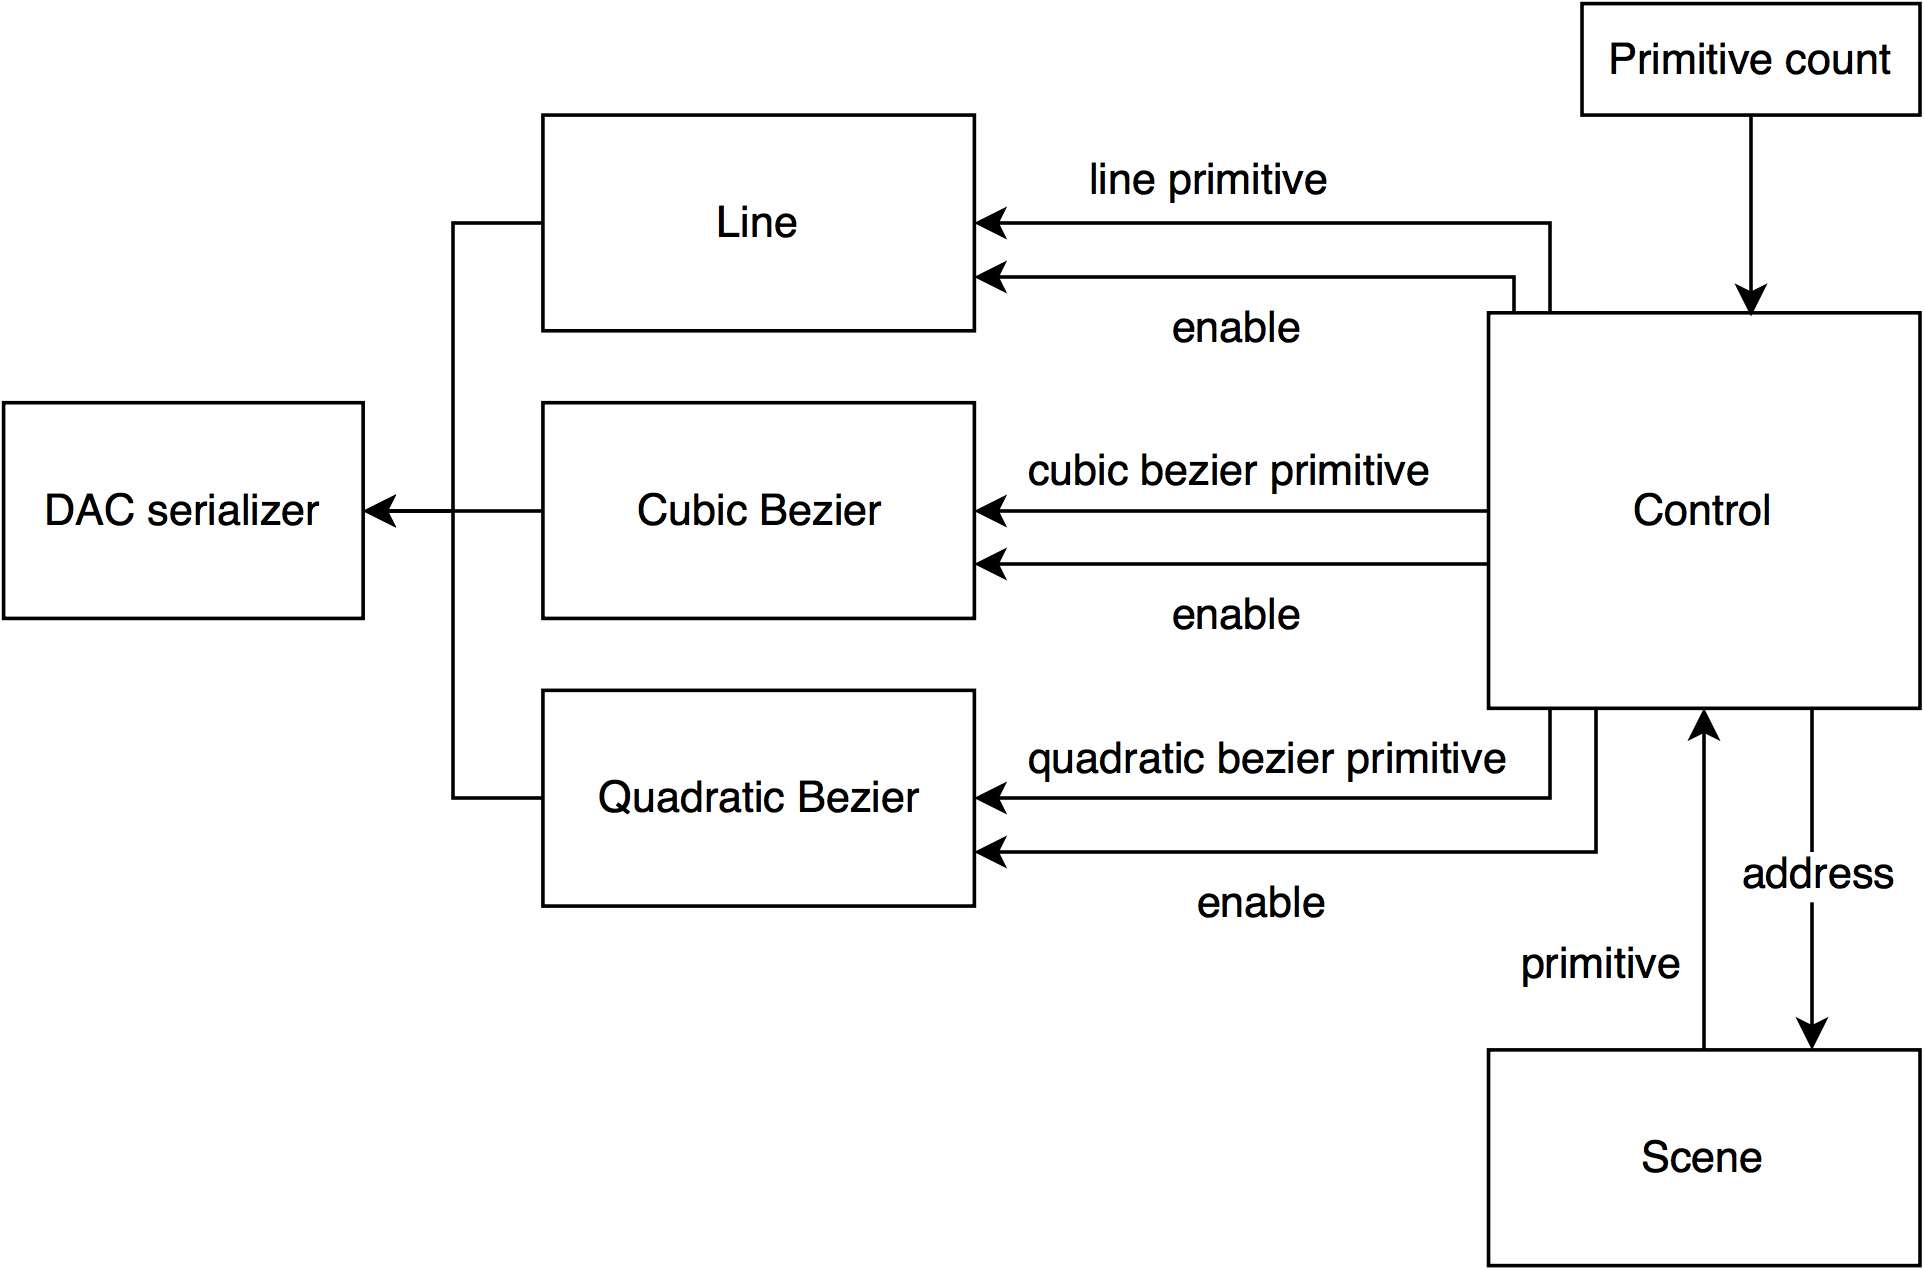
\includegraphics[width=\linewidth]{images/dac-output.png}
    \caption{\gls{rtl} sketch of the \vthreek \gls{dac} output module.}
    \label{fig:dac-output}
\end{figure}

The primary output of the processor is the analogue output.
This output is driven by two \gls{dac}s that converts digital data from the \gls{fpga} to voltages that represents x and y coordinates.
The \gls{dac}s used are 16-bit which results in an effective resolution of 65536 by 65536 without taking into account the noise on the output voltage which is explained further in Section~\ref{sec:noise}.
These \gls{dac}s have a serial interface and needs 3 signals each to operate; data, clock, and a sync signal.
In order to set an output value on a \gls{dac} the sync signal needs to be pulled from high to low then it needs 8 control bits followed by 16 data bits.
After this, the sync signal need to be pulled high again in order to set the output value.
The sync signal can be pulled high before this in order to abort the operation.
Clock and sync signal are shared between the \gls{dac}s in this system in order to make them change their output synchronously.

\subsection{Operation}

The output module send an address to the scene memory and gets a primitive back.
There is also another input that keeps track of the number of primitives so the module can restart without reading unused primitives.
It then decodes the primitive and forwards it to the appropriate module or reads a new primitive if no primitive was found and forwards the output of this module to the \gls{dac} serializer.
The respective serializer will then calculate a fixed number of points along the line or curve.
A fixed number of points was chosen because there was no time to implement any functionality for calculating the lengths of lines or curves accurately.
This will result in shorter lines and curves appearing brighter on the oscilloscope.

The actual calculation of the points is done by using the equations described in section \ref{sec:bezier}.
However since there was no floating point unit, a number between 0 and 1023 was used instead of a number between 0 and 1, that was then left shifted by 5.
\(t\) then becomes \(t = i \ll 5\) (\(0 \leq i < 1024\)).
After every multiplication the result is then right shifted by 15.
This results in a limit of 1024 different points for a given primitive.

The calculation for points for every type of primitive is largely the same, however the different number of points per primitive needs to multiplied by a different factor.
The equations for these can be found in Section \ref{sec:bezier}

\section{Raster Output}

This output uses \gls{hdmi} to output a rasterized image of the internal vector representation.
In order to generate the rasterized frame the x and y output from the vector output described in the previous section would be written into a frame-buffer.
This buffer can then be scaled to the desired output resolution and then sent over a regular HDMI connection.

\chapter{Microcontroller}

To handle I/O (not including output explained in Chapter \ref{chap:Output}), \vthreek is equipped with a microcontroller unit (MCU).
This chapter will explain the reason for including this part, and its responsibilities. 

\section{Silicon Labs EFM32 Giant Gecko}
A requirement for the assignment was to utilize a Silicon Labs EFM32 MCU to act as an I/O processor, listed in Figure \ref{lst:non_func_req}.
The EFM is a System on a Chip, and contains a 32-bit ARM Cortex-M3 processor, 1024kB flash memory and 128kB RAM \cite{efm32referencemanual}.

The Giant Gecko version was chosen for \vthreek.
The primary reason for choosing this variant of the EFM32 Gecko series, is that the EFM32GG DK3750 development kit was available for the team to test on from the beginning of the project.
It is the most powerful MCU in the series, and thus provides the most possibilities \cite{efm32}.

\section{Responsibilities}
The MCU does not have many responsibilities, and will in fact idle most of the time. The program flow is represented as a state diagram i Figure \ref{fig:mcu_state}.
Its primary tasks are: 
\begin{itemize}
\item Load program instructions into SRAM
\item Wait for button or joystick presses and react to these.
\item Controlling the status of the processor
\end{itemize}

\subsection{Loading program}
In order for the processor to do anything useful, we of course need to tell it what to do.
The program is contained within a header file in the MCU flash.
After the MCU has booted and initialized the subsystems it utilizes, it will wait for a \texttt{Done} signal from the processor.
This signal tells the MCU that JTAG has completed the FPGA flash process. 
It is important to wait for this signal, because the state of any signal connected to the FPGA is undefined prior to flashing.
This could possibly interfere with the MCU writing to SRAM.

Once the FPGA is flashed and ready, the MCU deasserts the Processor enable signal, to prevent it from start reading from SRAM prematurely.
The MCU now write the program to SRAM, starting at address \texttt{0x0000}, writing 16 bits at a time.
When complete, the Processor enable signal is asserted, and the processor will begin fetching instructions

\subsection{Buttons and joystick}
The board is equipped with two push buttons and a 5-way joystick, connected to the MCU's general purpose input/output pins (GPIO).
These inputs can be programmed to do anything, but was initially designed for controlling pan and zoom of the primitives.
A more useful functionality for one button was discovered to be soft resetting the processor.

When the processor is in normal operation, the MCU does nothing, and enters Energy Mode 2, to save power.
When a button is pressed, an interrupt is generated, and the MCU woken to handle the interrupt.

\begin{figure}[h!]
\centering 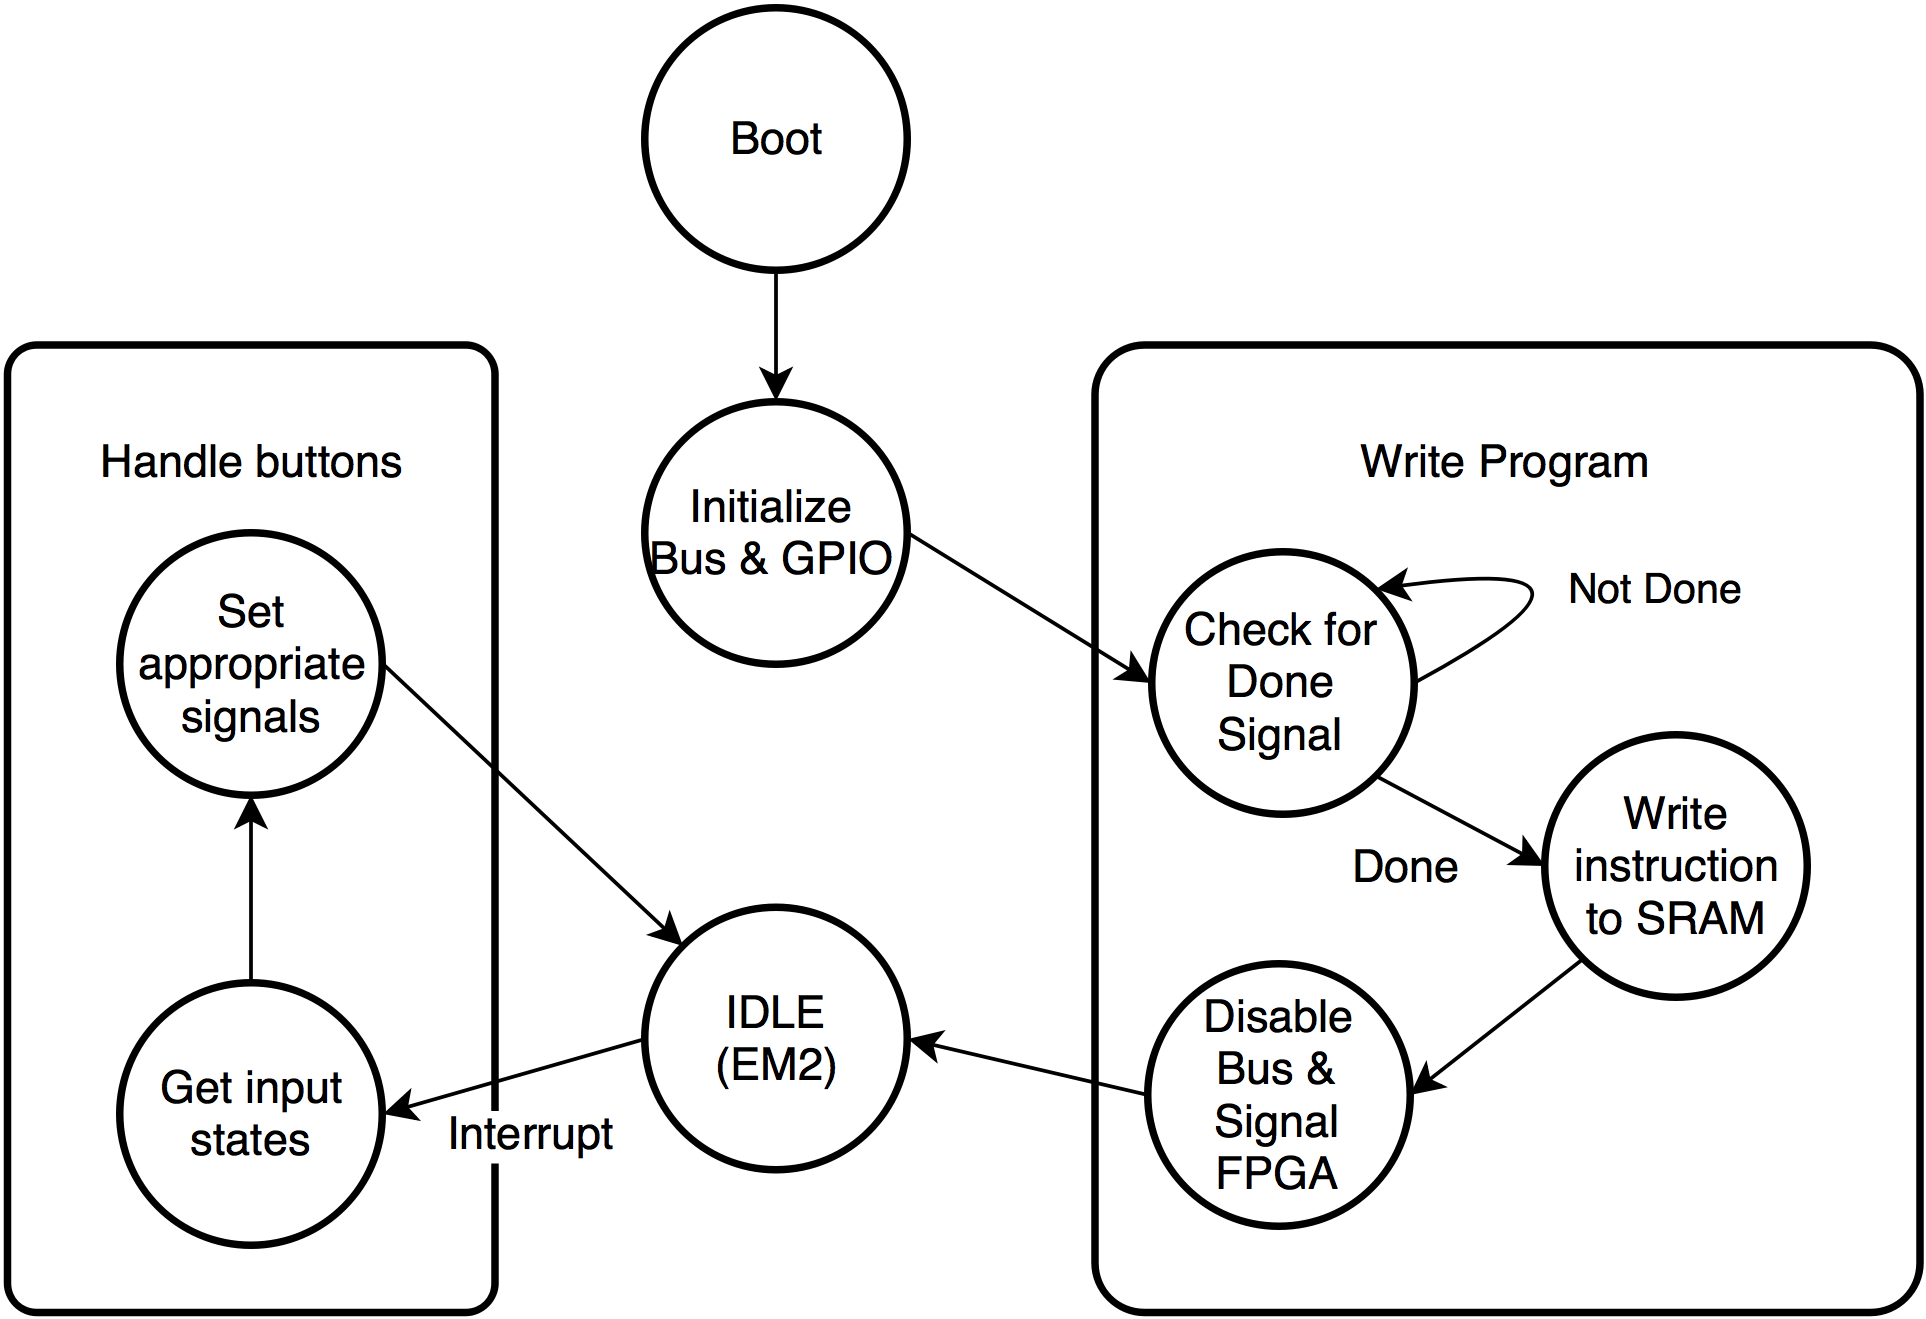
\includegraphics[width = 0.75\linewidth]{images/MCU_state.png}
\caption{The MCU program represented as a state diagram}
\label{fig:mcu_state}
\end{figure}
\chapter{Physical Implementation}

// TODO: add diagram of physical components and their connections

\section{Architecture}
The main specification the group had to meet at all costs was to be able to take a program (a sequence of instructions) as input, and output vector graphics on a screen.

Tracing the envisioned execution path of a program through the system gives insight into some of the considerations that had to be taken when designing the PCB and selecting components.

\begin{enumerate}
\item Assembled \vthreek programs are loaded into instruction memory via the EFM32 microcontroller.
\item The FPGA reads instructions from memory and performs execution.
\item The FPGA sends output via two interfaces, two DACs and an HDMI port.
\item The output from the DACs is displayed on an analogue oscilloscope and the output from the HDMI on a raster screen.
\end{enumerate}

\section{Components}
This section describes the team's choices of components.
All components had to meet the team's technical demands, e.g. number of pins, voltage level support and satisfying outputs.
This information was found by inspecting the various component's datasheets.
Critical components in the design are described in the following subsections.

\subsection{MCU}
The MCU was an EFM32GG microcontroller from Silicon Labs. 
It served as an input processor for our system, handling input before and during run-time. 
Some of the technologies included with it, were also exploited, for instance buses. 
//TODO: This information is included in mcu.tex. Could be merged?

\subsection{FPGA}
The FPGA was a Xilinx Spartan-6, with 401 kb block RAM. 
It served as the main processor in the design, fetching and executing instructions from instruction memory.
//TODO: Should the FPGA be introduced somewhere else?

A JTAG header was connected to the FPGA for good accessibility to FPGA debugging and programming.
//TODO : elaborate

\subsection{SRAM}
Two SRAMs were put on the PCB. 
One of them worked as an instruction memory for the FPGA, while the other was a dedicated frame buffer for our output signals. 
The instructions executed in the FPGA would update the frame buffer, and data from the frame buffer could be read and transferred to the output units. 
Both SRAMs had an address space of 512k 16-bit words. 

\subsection{DACs and BNCs}
As the purpose of the computer was to output vector graphics on an analogue vector screen, DACs were essential.
They would convert digital signals from the FPGA destined for the output screen, to corresponding analogue signals.

It was important that the DACs could output signals fast enough, to minimize flickering. 
Therefore, DACs that could support clock rates up to 30MHz was chosen.

The BNCs connectors would receive the analogue signals and send them to the oscilloscope.
There was one DAC and one BNC for both the x-coordinate and the y-coordinate on the oscilloscope.

\subsection{Oscillators}
Two external oscillators were connected to the MCU: one low frequency (32,768kHz), and one high frequency (48MHz).
The MCU already contained internal RC-oscillators, but external oscillators were much more accurate and stable than the internal ones, which was important for avoiding more sources of errors.
Both crystals or full-fledged oscillators could be used, but in the end, the team decided to use oscillators.
The reason behind this choice was that an oscillator was one fully built component with all the necessary circuitry inside, and the datasheet clearly specified how it should be connected.
Crystals, on the other hand, required load capacitors, whose values weren't properly specified.
Another reason was that our FPGA explicitly needed an external oscillator, as a crystal was incompatible with the design.
Hence, the team chose oscillators for both the FPGA and MCU for simplicity.

The FPGA oscillator had a frequency of 100MHz.
Even though this is a high frequency, this signal could be scaled inside the FPGA to desirable frequencies. // TODO: Elaborate?

\subsection{Buses}
The system used one parallel bus (EBI), and one serial bus (SPI).
The MCU acted as bus master for both of them, since it supplied the bus technologies.

\subsubsection{EBI}
The FPGA, MCU and SRAM were all connected via the EBI bus.
These connections were made properly by using the specified EBI-pins on the MCU. [citation to MCU datasheet]
The EBI bus allowed high-speed communication to the SRAM.
As the EBI bus is a parallel bus, the team included the following bus lines:
\begin{itemize}
\item 23 Address bits. More than initially needed, but this was increased for good measure.
\item 16 Data bits, since our SRAM consisted of 16-bit words.
\item 2 Chip select bits, one for the FPGA and one for the SRAM.
\item 1 Write enable bit, active low.
\item 1 Read enable bit, active low.
\end{itemize}

\subsubsection{SPI}
The SPI served as a three-way communication between the MCU, FPGA and Flash memory.
It's main purpose was to make the FPGA be configured from a bit-file stored in the flash memory.
As opposed to the EBI bus, SPI is a serial bus, transferring one bit of data at a time.

\subsection{Buttons and LEDS}
All buttons included a resistor for current limitation (to avoid short circuits) and pull-up (to avoid logical floating state).
The exception was the button connected to the MCU, where the pin had an internal pull-up.
All LEDs also included a current limiting resistor. 
Ohms law was used to calculate the required resistance\cite{ohm}.

LEDs were handy for giving an indication that something was turned on. 
For instance, the design included a LED which would light up when the FPGA was configured.
Buttons were used for triggering events, e.g. reset.

\subsection{Power Supply}
The PCB would receive power from a micro-USB connector. 
A voltage level of 5V was sufficient, since no components required more than this. 
However, plenty of components required less than 5V, specifically 3.3V. 
To lower the voltage to a specific level, voltage regulators were used. 
Power is discussed in more detail in section \ref{Power}.

\subsection{Decoupling Capacitors}
Several major components required decoupling, e.g. the MCU, FPGA, voltage regulators and DACs.
Decoupling means connecting power supplies through a capacitor network to ground, where power moving to ground can be temporarily stored.
This is necessary as it sometimes occurs situations where there is suddenly high need for power.
The power supply alone would not always be able to support these 'bursts'.
With a capacitor decoupling network, the component could pull power from the capacitors instead.

\section{PCB Design}
The architecture was realized on a printed circuit board (PCB) designed using Altium Designer 15.1.
Having never used this program before, the group had to overcome challenges and difficulties related to not only learning new software, but also learning concepts of creating a PCB from scratch. 

\subsection{Schematics}
The entire logic on the PCB was designed with schematics. 
Altium was used to map the components together, pin by pin. 
Making the right connections and pin mappings was the only thing that mattered in the schematics. 
There was no focus on physical PCB-specific things, e.g. routing and component placement.

When the schematics were completed, the team moved on to design the physical PCB.

\subsection{Component Placement}
The goal was to place the components on the PCB, so that they preferably were in close range of all other components they had to connect with. 
This would shorten the routing, which was desirable in terms of mitigating signal delay and maintaining signal integrity.

The FPGA, SRAMs and MCU were the most important components with a lot of different connections, and were therefore placed central on the PCB.
I/O components, e.g. controller buttons, USB, HDMI and BNC receptacles, were placed along the edge, since these were typically connected to few other components.
It would also be annoying to connect external peripheral plugs to sockets in the middle of the PCB.

All decoupling capacitors involved in the decoupling network for a certain component, were placed in close proximity to that component.
This minimized the risk of that the component wouldn't get the extra power supply it needed during bursts.
All capacitors and resistors were placed on the bottom layer of the PCB to save space on an already crowded top layer.

\subsubsection{Component Footprints}
A component footprint is how the trace of a component looks like on the PCB.
In the beginning, component footprints from the standard Altium library were used.
After previewing the board, it became clear that these footprints were in fact gigantic, and footprints of suitable size had to be found using Altium vaults.
Smaller 0603 (1608 metric) footprints were used for most passive components, especially the capacitors and resistors.
By standardizing footprint sizes, the bill of materials could easily be updated without changing the PCB design, as long as the new component could be found in the same package size.
While a trade-off by using this small size package is that the components might be trickier to solder onto the board, the gain in size reduction for the board as a whole were valued higher by the group.
Some components could not be found in this footprint, but luckily there was no shortage of footprint sizes to choose from.

\subsection{Layers}
The PCB consisted of six signal layers: Top layer, bottom layer and four in between.
Two power layers were utilized: \(V_{CC}\) and ground.
Between every signal and power layer, a dielectric layer was added to ensure proper isolation between these conducting layers, such that they wouldn't interfere with each other.

An overlay was added to both the top and bottom layers.
The overlay was added to contain silk-screen for marking components, thus making it easier to navigate the PCB.

The complete layer stack is shown in figure \ref{fig:Layers}

\begin{figure}[h!]
\centering
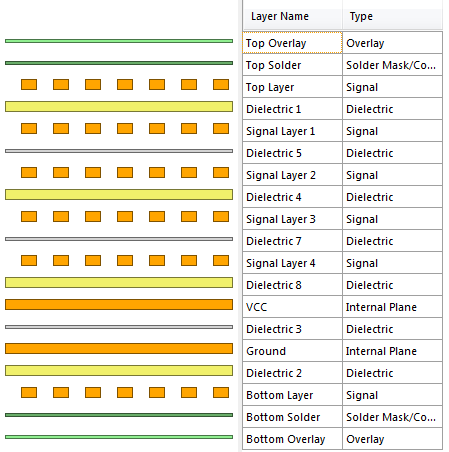
\includegraphics[scale = 0.8]{images/Layers.png}
\caption{Layer Stack}
\label{fig:Layers}
\end{figure}

\subsubsection{Power and ground}
\label{Power}
The PCB was designed with three power domains, each with their corresponding voltage regulator: 3.3V, 1.2V and a 5V reserved for analogue signals.
Most components were supplied by the 3.3V regulator, except for some internal parts of the FPGA that required 1.2V.

Since 3.3V was used by most components, and since only a few connectors required 1.2V, a dedicated power plane for 3.3V was added.
A dedicated ground plane was also added.
This prevented more unnecessary routing, since everything connected to 3.3V or ground could go straight to a via by dogboning, and automatically be connected to the corresponding plane. 
The 1.2V traces had to be routed through all the connectors like any other signal. 

\subsubsection{Split planes}
The story of analogue 5V is a little different. 
The reason for an analogue 5V was to avoid noise from digital signals. 
The analogue components are sensitive to noise from the digital circuitry, and it was crucial to have as little noise as possible on the signal going to the oscilloscope. 
To avoid noise, the analogue and digital circuitry had to be separated completely. 
Analogue components could not use the same voltage supply as the digital ones, and the same mattered for ground.

The solution was to split the power and ground plane, shown in figure \ref{fig:Split planes}. 
\begin{itemize}
\item 5AV: Analogue 5V for components on the analogue plane. 
The reason for 5V was based on insecurity about how much voltage the oscilloscope required to properly display the vector graphics from the program. 
3.3V could be too low, so 5V was chosen. 
A high signal voltage could also potentially help reduce noise.
\item AGND: Analogue components are connected to this ground instead of digital ground. 
This is to stop the analogue signal from getting disturbed by the digital signals on the ground plane.
\item 3.3V: Digital voltage for digital components.
\item GND: Digital ground.
\end{itemize}

All analogue components were placed in the analogue plane, and the opposite with digital components. 
The exception was the DACs, which acts as a bridge between the digital part and the analogue part. 
These were placed on the actual split, with the affected pins on the correct side.

To remove any digital noise that could potentially accumulate on the analog ground plane, a diode was placed between the two ground planes. 
This let the current flow from the analogue ground to the digital ground, but not vice versa.

\begin{figure}[h!]
\centering
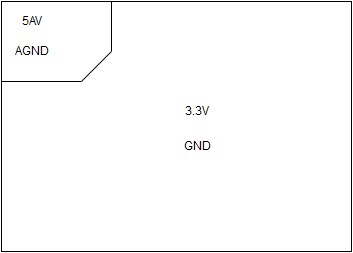
\includegraphics[scale = 0.6]{images/Split_planes.png}
\caption{Split between analogue and digital planes. The separating line is a solid, non-conducting material}
\label{fig:Split planes}
\end{figure}

\section{Routing}
The components had to be physically connected according to the schematics.
Connections could be manually routed, or Altium's auto router could be used. 
The auto router would automatically route as many connections as possible.  

Routing was a much more time-consuming process than the team expected. 
Too much trust was put into Altium's auto router. 
The router did not, as the team naively thought, magically solve the routing. 

\subsection{Design Rules}
Before routing, necessary rules had to be defined to make sure the PCB was routed properly. 
The following listing explains the most important rules for the design.
\begin{itemize}
\item Clearance: 0.1mm. 
\newline
Minimum clearance between different traces
\item Width: 0.127mm, Power Width 0.203mm.
\newline
Minimum width for traces. 
Power traces had bigger minimum widths, than signal traces.
\item Via Diameter: 0.4mm, Via Hole Size: 0.2mm
\newline
Minimum diameter and hole size for multi-layer vias.
\item Short-circuits and net antennas not allowed
\end{itemize}

The rules were set like this to make sure there wouldn't be any interference between traces, while the traces were still wide enough to not be damaged by the signal itself. 
Power traces were wider to make sure they could handle the voltage.
Net antennas were traces that lead to dead-ends. 
This could harm the design, since these dead-ends could work as unwanted signal receivers from nearby sources.

\subsubsection{Design Rule Check}
Altium had it's own tool for testing how many violations our current design created, called Design Rule Check. 
It displayed the amount of errors occurred from each type, and the coordinates on the PCB for every error. 
Typical errors during our design procedure were short-circuits, net antennas and clearance constraint violations.

\subsection{Routing Procedure}
The task of routing the PCB was started by routing some components manually. 
The team quickly discovered that doing this for the entire board would take a very long time, and so began to check out Altium's built-in auto router. 

Roughly, this routing procedure was followed:
\begin{enumerate}
\item Run the auto router.
\item Run Design Rule Check, and observe how many errors that occurred. 
\item If there are too many errors (e.g. more than 200), there is most likely something wrong with the design rules or the auto router settings. If not, go to step 6.
\item Check and modify settings and rules.
\item Go back to step 1.
\item Go through the remaining errors and fix them. 
\item ...
\item PROFIT!
\end{enumerate}

The team ran into many different routing problems, which is discussed in detail in section \ref{Routing Problems}

\section{Fault Handling}
The team were all inexperienced with PCB design and often uncertain if actions or decisions could cause problems down the line. 
The top priority was to make something that worked properly. 
A failing component was deemed probable, and forgetting something was guaranteed to happen, considering the vast amount of factors involved. 
Hence, the team decided that having back-up features on the PCB was critical.

\subsection{Headers}
The primary strategy of handling faults was redundancy, mostly in the form of header pins. 
The final amount of headers ended up at 34, including the JTAG and the ARM programming header. 
Using this huge amount of headers made it possible to measure most signals with a multimeter and verify them. 

Most headers were placed between components. 
If wrong connections existed, or a connection didn't work, the connection could hopefully be corrected by connecting wires. 
Not only could errors more easily be detected - it would also be easier to fix them.

\begin{figure}[h!]
\centering
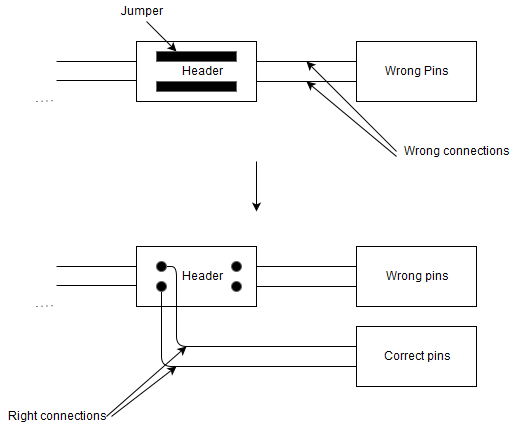
\includegraphics[scale = 0.45]{images/Header_fix.png}
\caption{Example Header fix}
\label{fig:Header fix}
\end{figure}

Headers was also useful as switches. 
By manually connecting header pins with jumpers, certain parts of the PCB could be activated and deactivated. 
This would be useful when focusing on lesser parts of the circuit. 
For instance, 3-pin headers were used to manually turn on and off different voltage levels. 
Power could also be delivered to the components directly through the headers, if any issue with the power supply should occur.

\subsection{DACs}
Even though separate DACs for outputting analog voltage out to the BNC plug was included, there was still a risk that the group could not get them to work. 
A back-up solution by connecting the internal DACs in the MCU to the BNCs was implemented. 
One 2x2 header for each BNC input was used to manually control whether the main DACs or the MCU DACs were to be used. 
This process is shown in figure \ref{fig:DAC headers}. 
There's one header each for the X and the Y signal to the oscilloscope. 

\begin{figure}[h!]
\centering
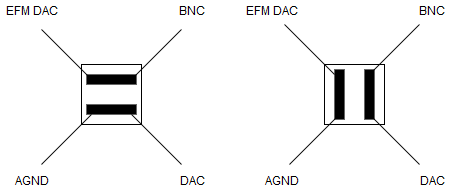
\includegraphics[scale = 0.6]{images/DAC_headers.png}
\caption{Left: Jumpers connecting MCU DAC to BNC and normal DAC to ground.
         Right: The opposite}
\label{fig:DAC headers}
\end{figure}


\chapter{Tools}
The primary tools used during development are detailed in the following list. All software were used in the latest version available to us at the time (fall 2015), unless specified otherwise.
TODO: Fill in all the tools used.

\begin{description}
    \item[Simplicity Studio] For development and programming EFM32 chip.
    \item[Altium Designer] For creating the PCB
    \item[Git] For collaboration and version control. Github was used as a repository manager.
    \item[Xilinx ISE] For writing and syntax checking VHDL
    \item[Xilinx ISim] For testing simulated modules in testbenches
\end{description}

\section{Assembler}
Initially the group wanted to create a compiler and have a higher level language.
Due to the time constraint only assembler were created.
As the group wanted specialized vector instruction, an unique instruction set were created.
The instruction set also contains more general instructions like branch and jump.
The assembler takes each instruction and converts it into 32 bit binary instruction words.
A complete ISA overview can be found in appendix \ref{app:isa}.


% Part III
\part{Results}
\chapter{Testing}
This chapter will present the testing performed on the system. It will explain the methods we used and some of the results.

\section{IO Tests}
Before our PCB board arrived we tested each subsystem separately.
During testing the group gained valuable experience about all the subcomponents and how they interacted with each others.

\subsection{DAC}

\subsubsection{Without the PCB}

The DAC was tested prior to PCB arrival, to ensure correct operation from an FPGA.
Eight wires were soldered onto the DAC, and connected to a breadboard.
The FPGA was flashed with and simple architecture, which repeatedly read the status of 14? general I/O pins, and shifted each bit out sequentially on another pin.
Both the DAC and FPGA clock input was driven by an external frequency generator, producing 3.3VPP at 10MHz.

To validate the signal output from the FPGA a logical analyser was used.

With VRef and VDD at 5.0V, the analogue DAC output was measured to 0.69V when no data signal was asserted, and 2.8V when the MSB was asserted. This small offset, is the result of some of the lower order bits being left unconnected.

\subsubsection{With the PCB}

Once the the PCB arrived we were able to test the DACs soldered onto the PCB as well as with actual data from the FPGA.

Clocking data from the FPGA to the DACs on our PCB presented some issues as we hit a limit in the Spartan 6 architecture regarding clock routing. This was resolved by using an ODDR in order to forward the clock signal to the desired output pin. //TODO: Ref for ODDR

Once we had the data input to the DACs working we could test the outputs. In does this we found some issues with out ground planes as well as the maximum output voltages from the DACs. The maximum voltage we were able to get was 1.6V, a little under half of our reference voltage of 3.3V. //TODO: Update this when the problem is fixed.


\subsection{Oscilloscope}
As a proof of concept to draw on an oscilloscope, we created a 4-bit resistor ladder DAC. The schematic of the DAC is displayed in Figure \ref{fig:r2r-ladder}.
An Arduino was used to control the DAC.

To test drawing on both x-axis and y-axis, the circuit consisted of 2 4-bit DACs.
With a small Arduino program we were able to draw a square, depicted in Figure \ref{fig:osc_poc}.
When the Arduino changed the voltage on its GPIO pins, there was a voltage drop across all pins.
The consequence of the voltage drop is clearly visible (see Figure \ref{fig:osc_poc}).


\begin{figure}[h]
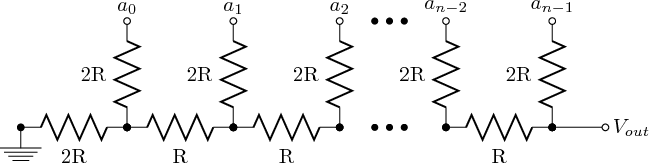
\includegraphics[width=\columnwidth]{images/r2r-ladder}
\centering
\caption{Schematics of the resistor-ladder\cite{r2r-ladder-schematics}.}
\label{fig:r2r-ladder}
\end{figure}

\begin{figure}[h]
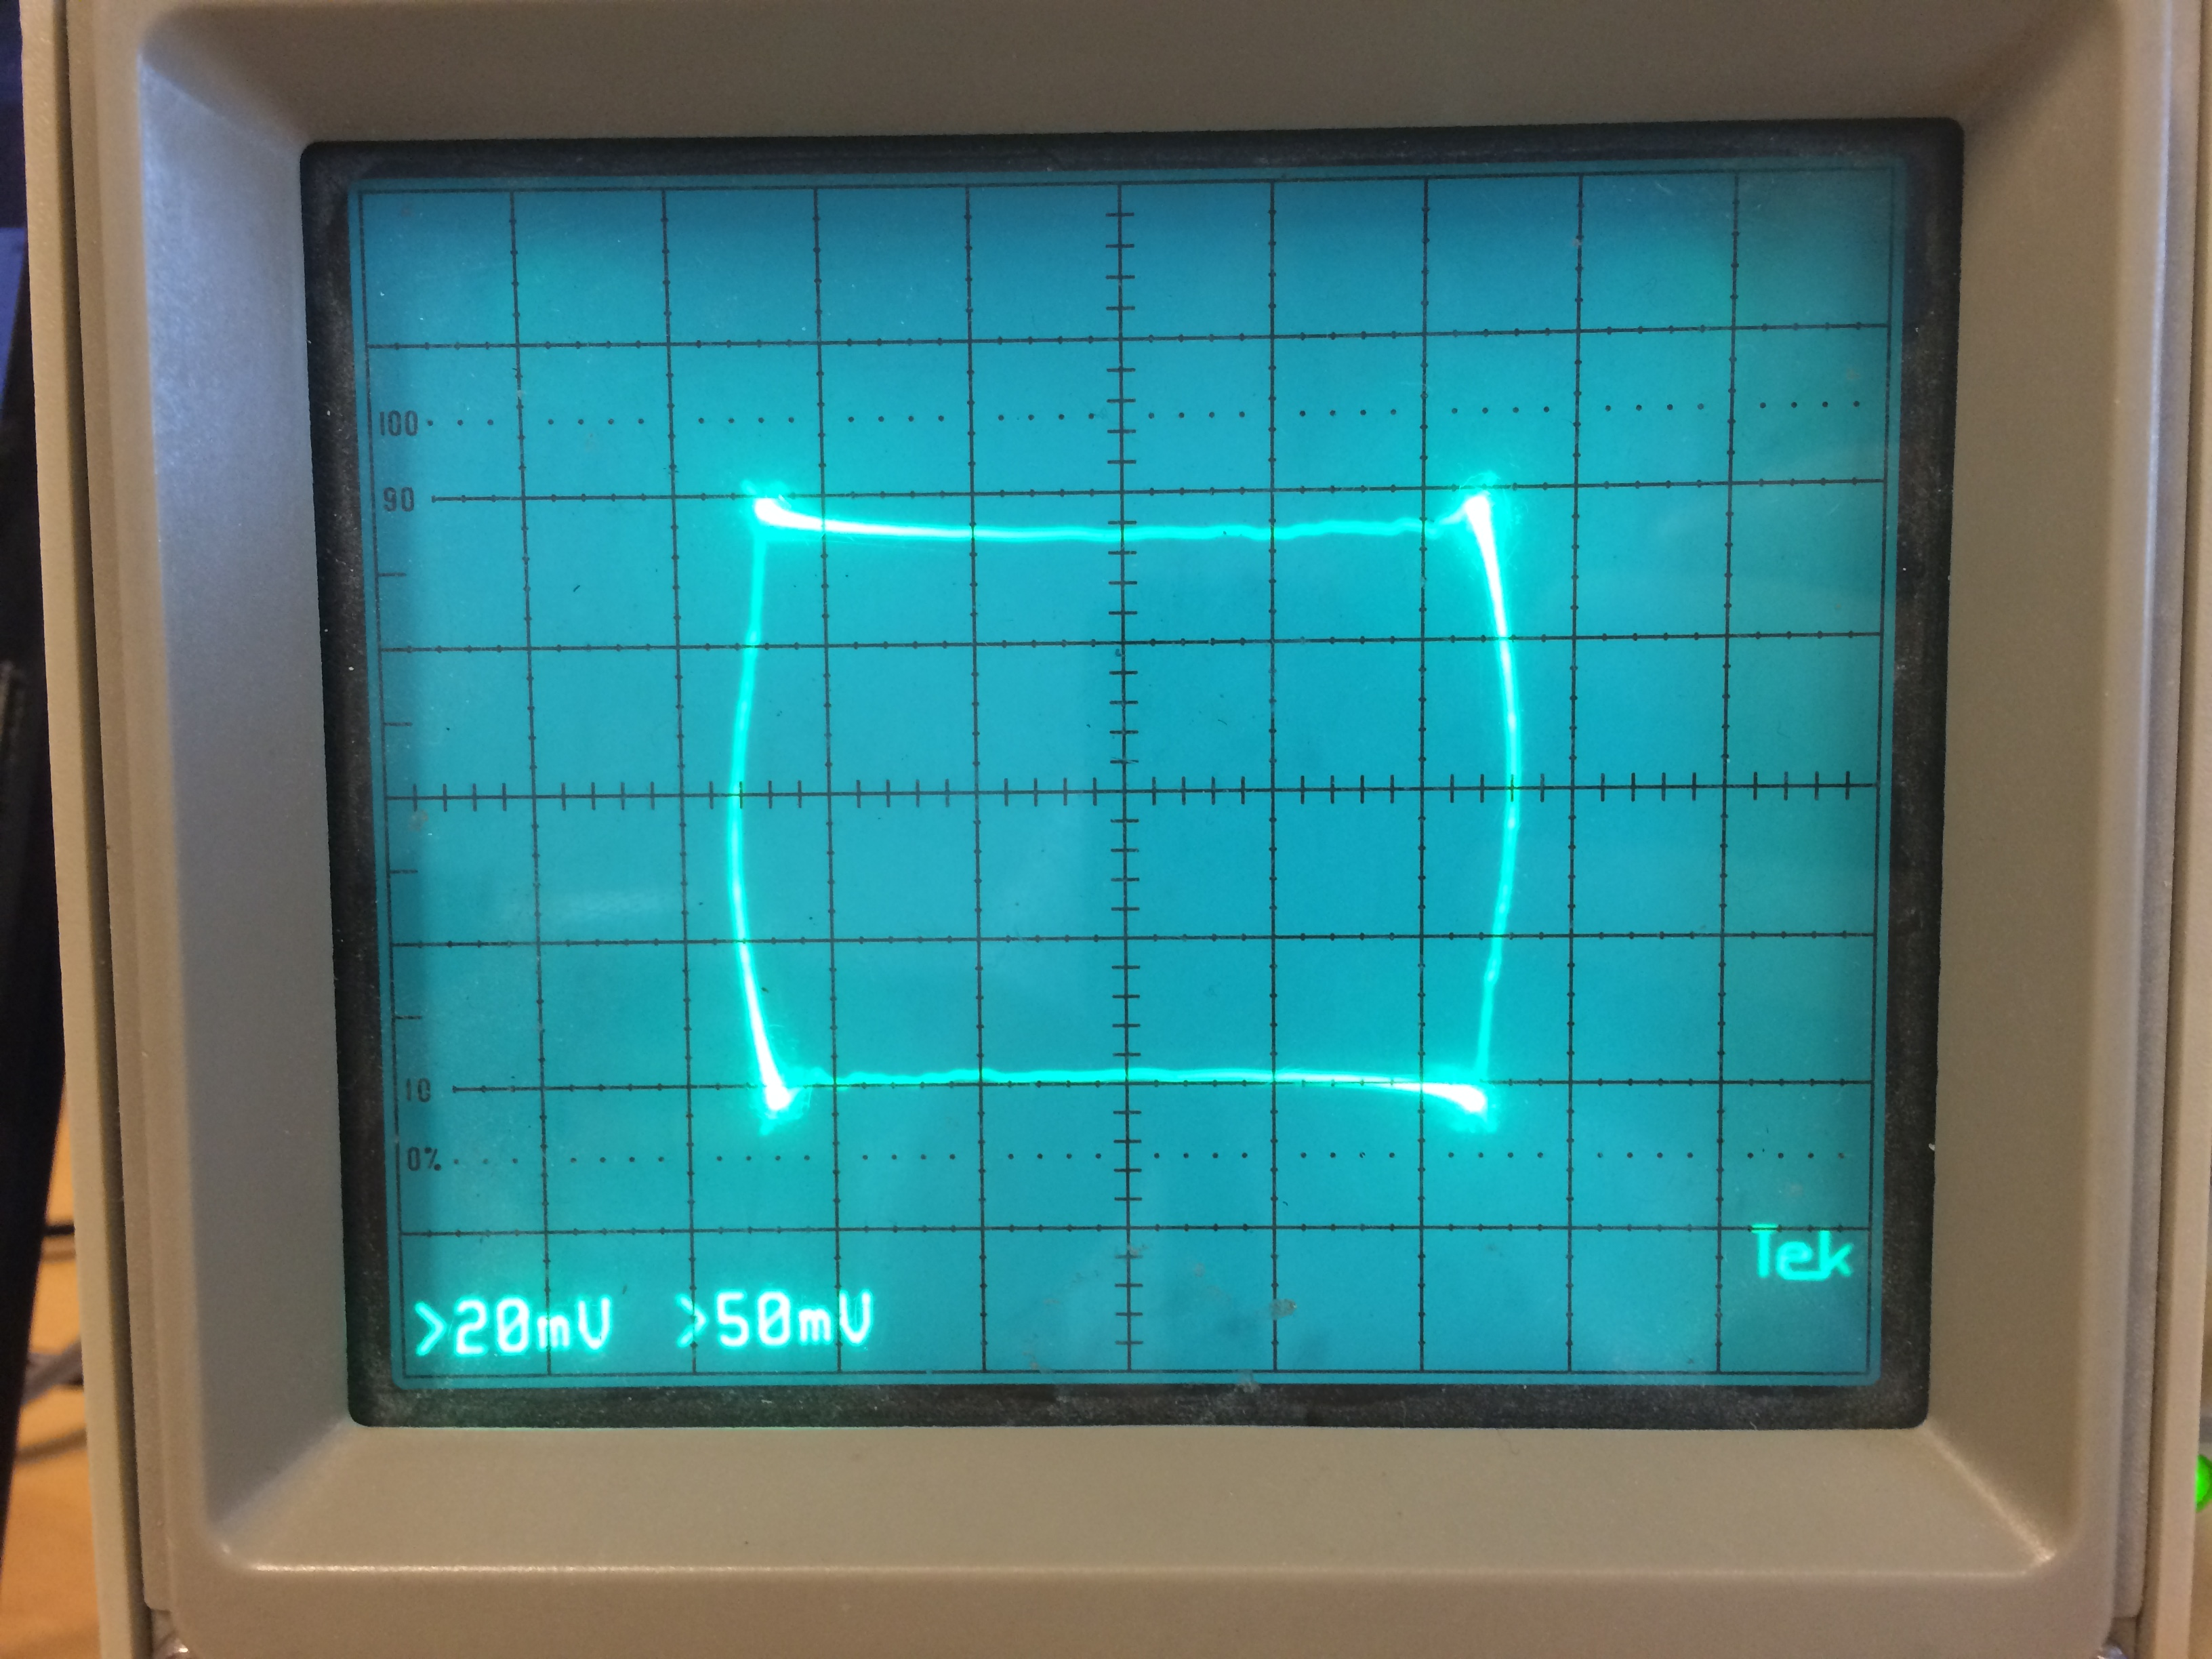
\includegraphics[width=\columnwidth]{images/osc_square_close}
\centering
\caption{A "square" drawn on the oscilloscope using an Arduino and two resistor-ladder DACs}
\label{fig:osc_poc}
\end{figure}

\section{Physical PCB and Components testing}

// TODO: Restructure this, some of it belongs in results, some in discussion.

When we had received the PCB and the components, we had to make sure that every component worked properly independent of the PCB, then testing if they worked on the PCB. Many major components were impossible to test without soldering on the PCB though. Examples were the FPGA and MCU, because of their tiny ball grid pins.

\subsection{Soldering}
There were different ways of soldering components on the PCB. It depended on components being through hole, surface mounted, pin size, etc.
\subsubsection{Ball Grid Arrays (BGA)}
Both the FPGA and MCU were ball grid arrays.
Therefore, they were soldered on the PCB,//TODO: No paste were smeard by smearing paste over the corresponding area, putting them carefully on, and putting the PCB in a heater. The heater made the components stick properly to the paste. This was the only way, since soldering pins directly under the component by hand, isn't practically possible.

\subsubsection{Surface Mounted Components}
Most surface mounted components where the pins weren't too small and crowded, were soldered by hand. Paste were used before hand, just like with BGAs, but after that the pins could be soldered by hand, since the pins were within physical reach. 
\newline
If pins were too small and tight, the same technique was used as for the BGAs.

\subsubsection{Through Hole Components}
Through Hole components were the easiest to solder, since the pin size and the space between them was relatively large. Additionally they were on the bottom side of the board. No paste was needed, each individual pin could be soldered with tin wires.

\subsection{Testing}
We had to find and fix all errors and faults with our PCB design and components, that were a hazard to our desired resulting system.  
We ran tests during our soldering process to make sure the system so far worked desirably. Running tests during the process, lowered the amount of potential sources of errors, which made it easier to discover errors.

\subsubsection{Power Planes}
It was very important to verify that the power planes worked as we intended. Obviously, nothing would work without power. Hence, this was the very first test we performed.
\newline
Everything necessary for power to be present, was soldered on. This included power headers, and the 3.3 voltage regulator. External power was inserted through power headers. By measuring different places with a voltmeter, we already discovered anomalies. The voltmeter showed only 2.3V instead of 3.3V. Further testing revealed that one of the voltage regulator pins hadn't been soldered properly, resulting in a loss of 1V. After fixing this, the digital VCC plane contained the correct 3.3V.


\section{PCB Design Flaws}
No project would be complete without something going wrong. Our project is no exception. After receiving our manufactured PCB, we started to discover various complications. This section discusses the more serious ones in detail, and what we did to solve the problem.

\subsection{Incorrect Wiring}
We discovered that our buttons was wired wrong, since they caused short-circuits. The reason was sloppy study of the datasheet, as shown in figure \ref{fig:Button Issue}. Luckily, this could be remedied by rotating the button 90 degrees, if we adjusted the physical connectors to fit the footprint.

\begin{figure}[h!]
\centering
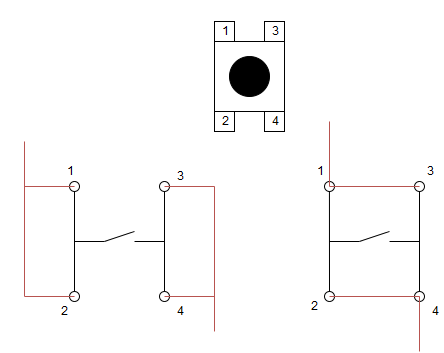
\includegraphics[scale=0.5]{images/Button_Issue.png}
\caption{Top figure shows the button as it looks like on the PCB. On the left: Correct wiring according to datasheet. On the right: Incorrect wiring leading to short-circuit}
\label{fig:Button Issue}
\end{figure}

When testing the oscillators, they did not seem to work. The datasheet for these components clearly stated that connecting the E/D pin to either 'No Connect' or '1' equaled active, so we did not connect it. We tried to remedy by connecting E/D to Vcc, and the problem was solved.
\newline
\newline
The Vref chip was supplied with 3.3V, but should have been supplied with analogue 5V instead. This could be remedied by cutting on the 3.3V power trace, since the trace is located on the top layer and no other traces are beneath it. Then we could connect analogue 5V via header from the voltage regulator to the input pin on the Vref chip.
\newline
The DACs were supplied with analogue 5V, but should have been supplied with 3.3V. The analogue 5V should go to the Vref chip instead. Solved by switching the two connections.

\subsection{PCB Placement and Footprints}
The BNC connector's footprint was wrongly routed - ground and Vcc was switched on the PCB. We discussed inverting the signal, but found that switching the pins on the component was the easiest thing to do.
\newline
\newline
It would have been beneficial if we had placed the 3.3V voltage regulator closer to the JTAG debugging port, since the Xilinx JTAG platform cable required a 3.3V power supply.
\newline
\newline
The micro USB footprint originally contained mounting holes, but were wrongly removed before manufacturing. Luckily, these did not act as connectors, and we could therefore solder the USB receptacle onto the PCB like a surface mount component.

\subsection{Component Order Issues}
The initial LEDs we ordered were reverse mounted, meaning that they required a hole in the board and had to be soldered on to the bottom layer. Because of this, we had to buy some new ones.
\newline
\newline

\subsection{Component sizes}
In hindsight, it would have been better to order bigger components. Since this is a prototype board where we mostly solder by hand, an increase in size would only be beneficial for us. If the project should go into large scale production, we could have tried to shrink the size.




\chapter{Results}
The group ended up with a computer that managed to produce vector graphics according to design.
This chapter presents the results of the project.
The physical result is depicted i Figure \ref{fig:board-top}.
The advanced tunnel program that was produced (see Appendix \ref{app:tunnel}), can be seen in action here: \href{https://vid.me/JEZv}{https://vid.me/JEZv} \cite{tunnel-demo}.

\begin{figure}[h!]
	    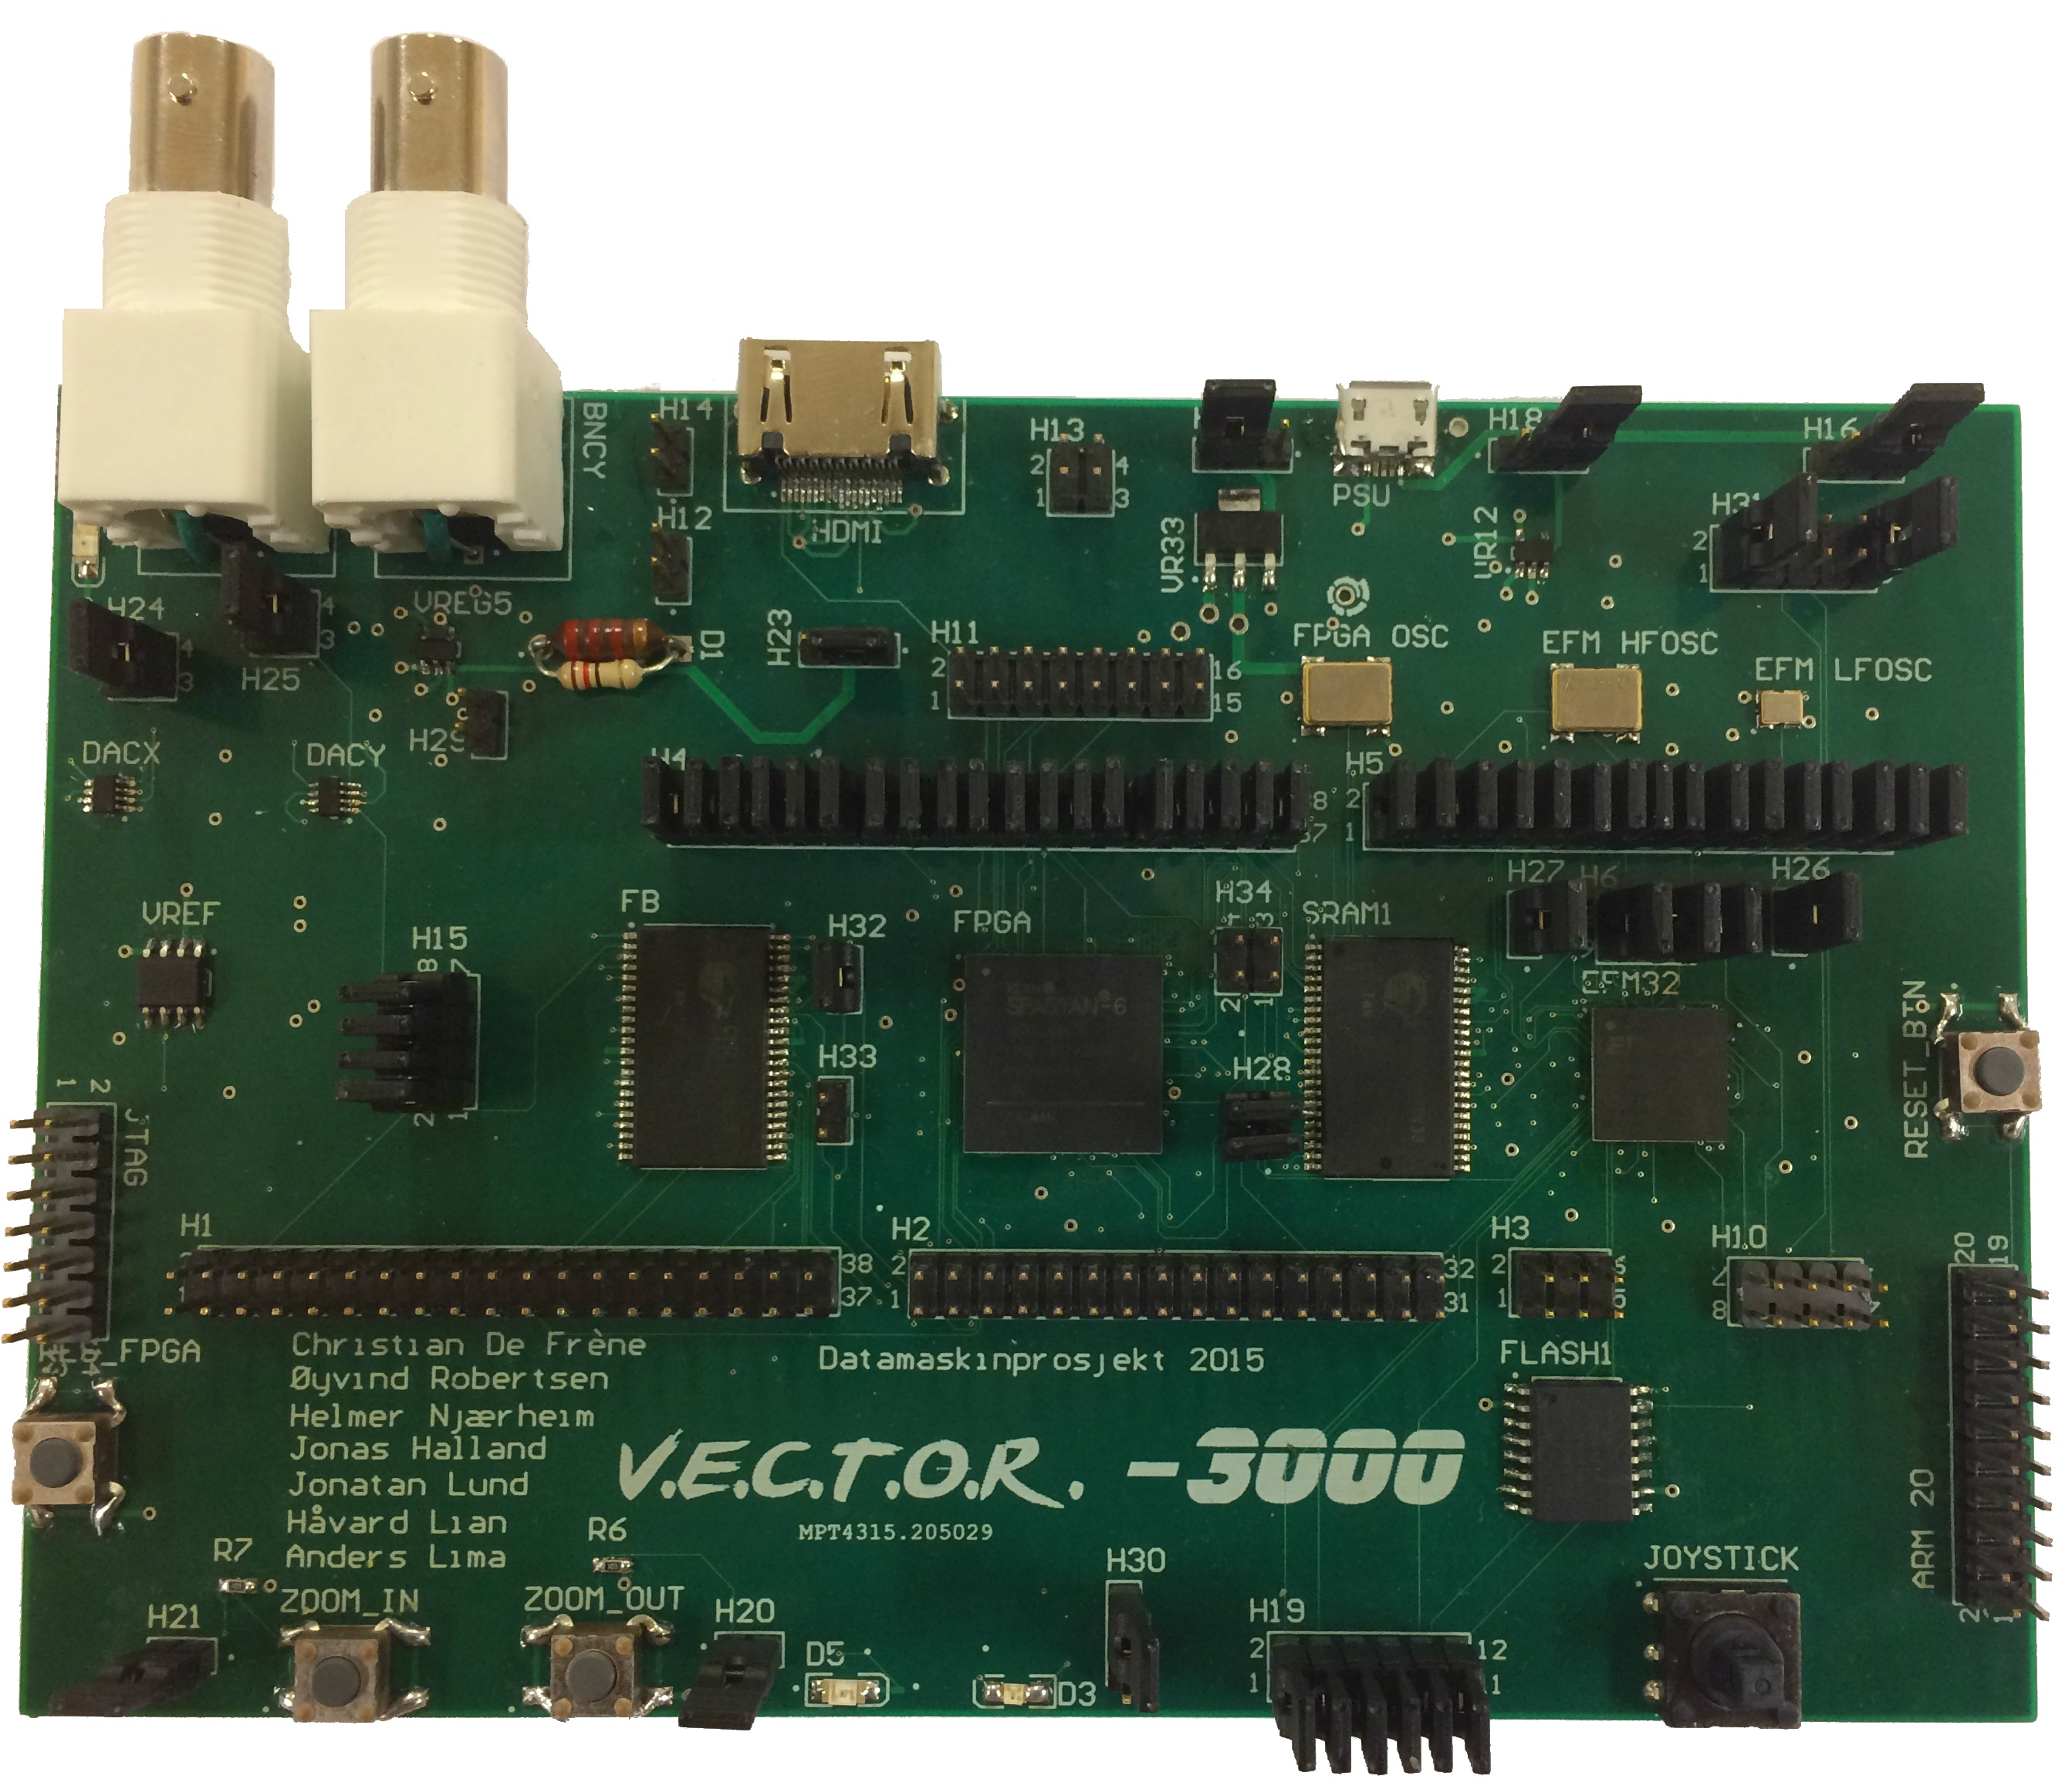
\includegraphics[width=\linewidth]{images/board_top.jpg}
	    \caption{An image of the finished \vthreek board}
	    \label{fig:board-top}
\end{figure}

\section{Memory}

The final implementation utilizes \gls{bram} not only to store the scene, but the instructions for the CPU as well.
This was done because to group was unable to get the SRAM chip that was on the three-way EBI bus to work properly.
Because of this the instructions for the CPU needs to be stored in the .bit file that programs the FPGA.

The SRAM chip dedicated to frame-buffer was also left unused as the group did not find the time to implement a raster output module.

\section{Performance}

The maximum clock frequency of the DACs is 30MHz according to the datasheet \cite{dac-datasheet}.
To update the DAC value a total of 25 clock cycles are required.
As a result the theoretical effective maximum output will be \(30 MHz \div 25 = 1.2 MHz \).
However during testing the group experience incorrect \gls{dac} values if the clock were set higher than 20 MHz.
With a clock frequency of 20 MHz the maximum output is 800 KHz.

The CPU can be clocked significantly faster than it is in the current design, but since the output module needs to be run at 20 MHz this was chosen for the CPU as well for simplicity.
At 20 MHz the CPU is still more than fast enough to update primitives in order to achieve smooth animations, so busy loops was introduced in the primitive update procedures in order to slow the update rate down.

\section{Noise}

As the main output is analogue it is susceptible to electronic noise. This noise represents itself as unwanted changes in voltage. 
The system was design to have as little noise as possible, and under operation the mean noise on the signal is around 40mV.
A measure of this is shown in Figure~\ref{fig:noise}.

\begin{figure}[H]
	    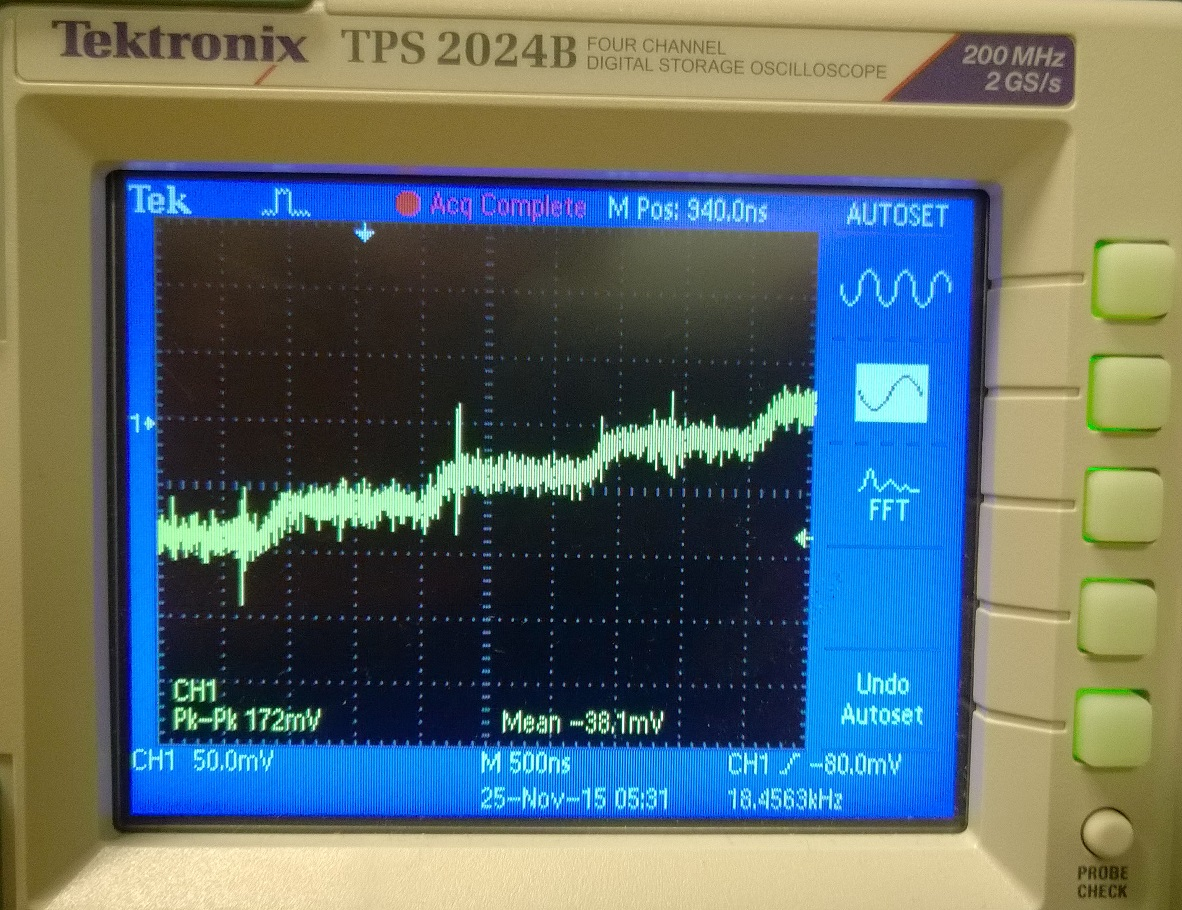
\includegraphics[width=\linewidth]{images/noise}
	    \caption{The noise on the voltages from the DACs}
	    \label{fig:noise}
\end{figure}



\section{Video Output}
\vthreek was successful in drawing primitives to a a screen.
Only one of the output modules, the analogue oscilloscope output, were realized.
This section presents the results from this module.

\subsection{Oscilloscope}
In Figure \ref{fig:square}, one can see great improvement in the accuracy when drawing a square, compared to the result in Figure \ref{fig:osc_poc}.

\begin{figure}[h!]
	    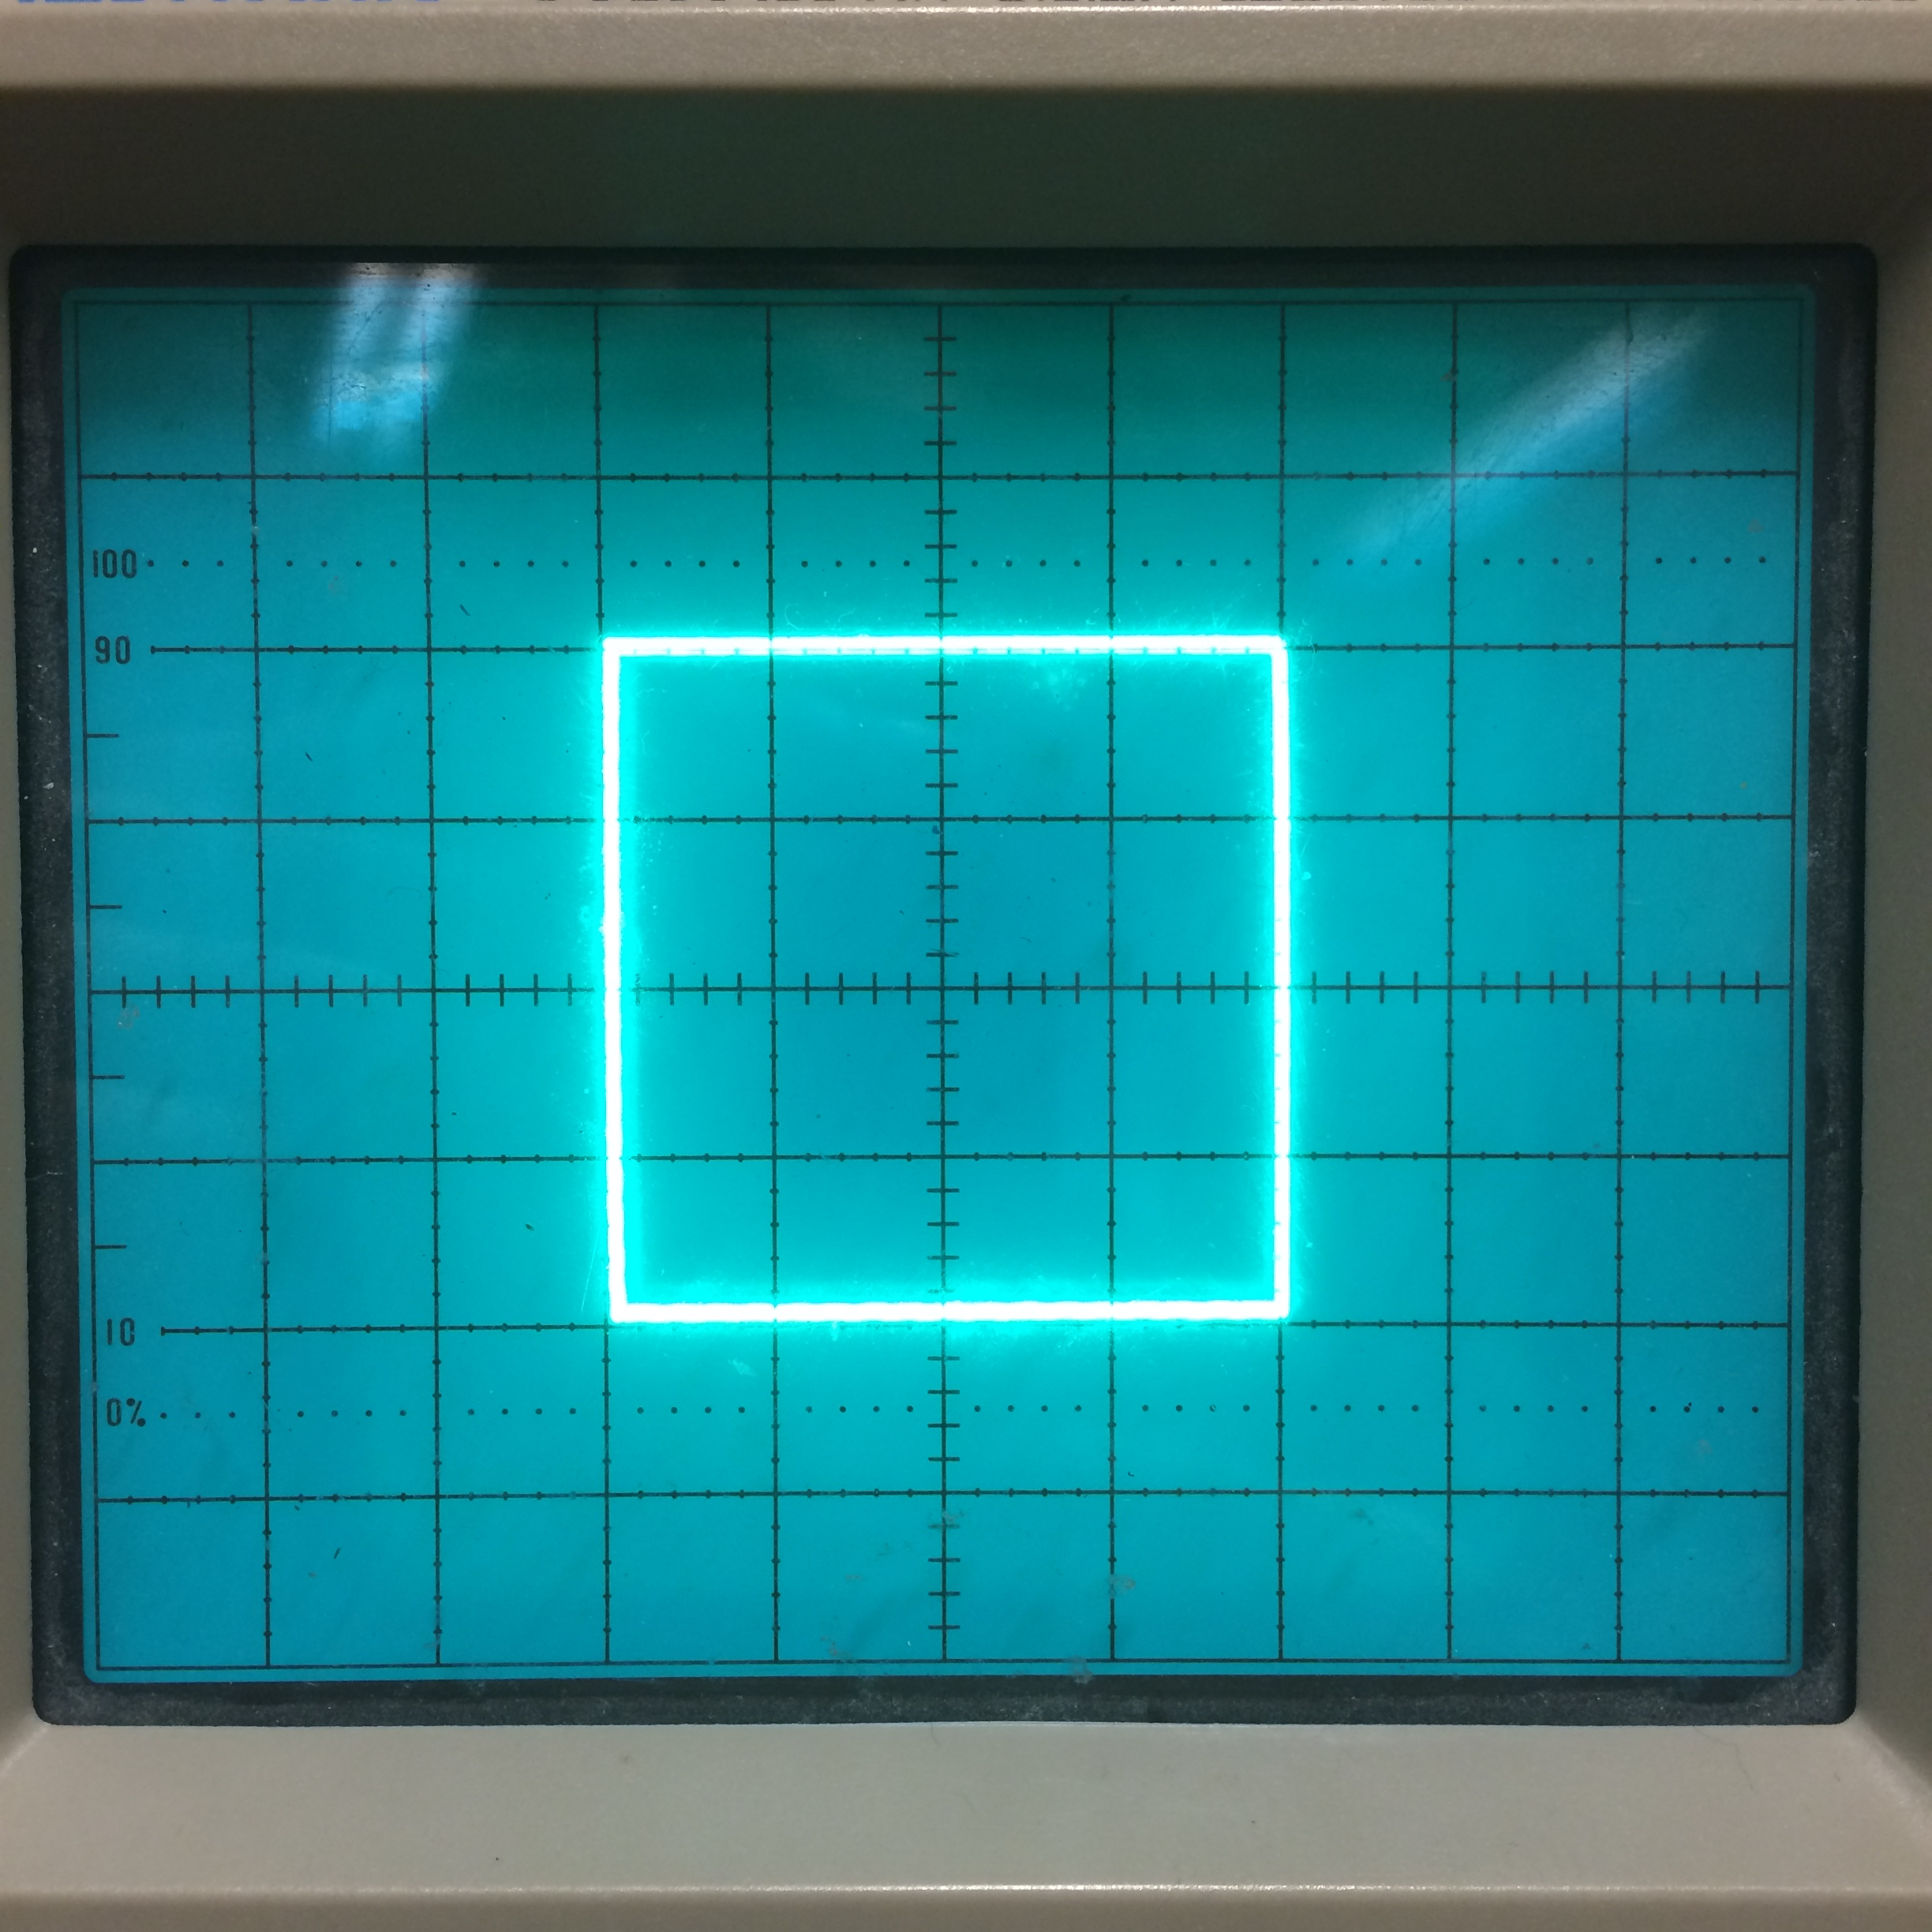
\includegraphics[width=\linewidth]{images/square}
	    \caption{A square drawn with the finished implementation}
	    \label{fig:square}
\end{figure}


\subsubsection{Drawing Artefacts}
\label{results:artefacts}
Even though drawing to the oscilloscope looks nice, some artefacts were discovered.
When the oscilloscope is done drawing one primitive and moves to the next the electron beam i still drawing,
and weaker drawing lines may be visible.
In other words all shapes are drawn without "lifting the pencil off the paper".
If one take a closer look at Figure \ref{fig:artefact}, the drawing artefacts are visible.
There are solutions to avoid the drawing artefacts, which is explained in Section \ref{discussion:artefacts}.

\begin{figure}[h!]
	    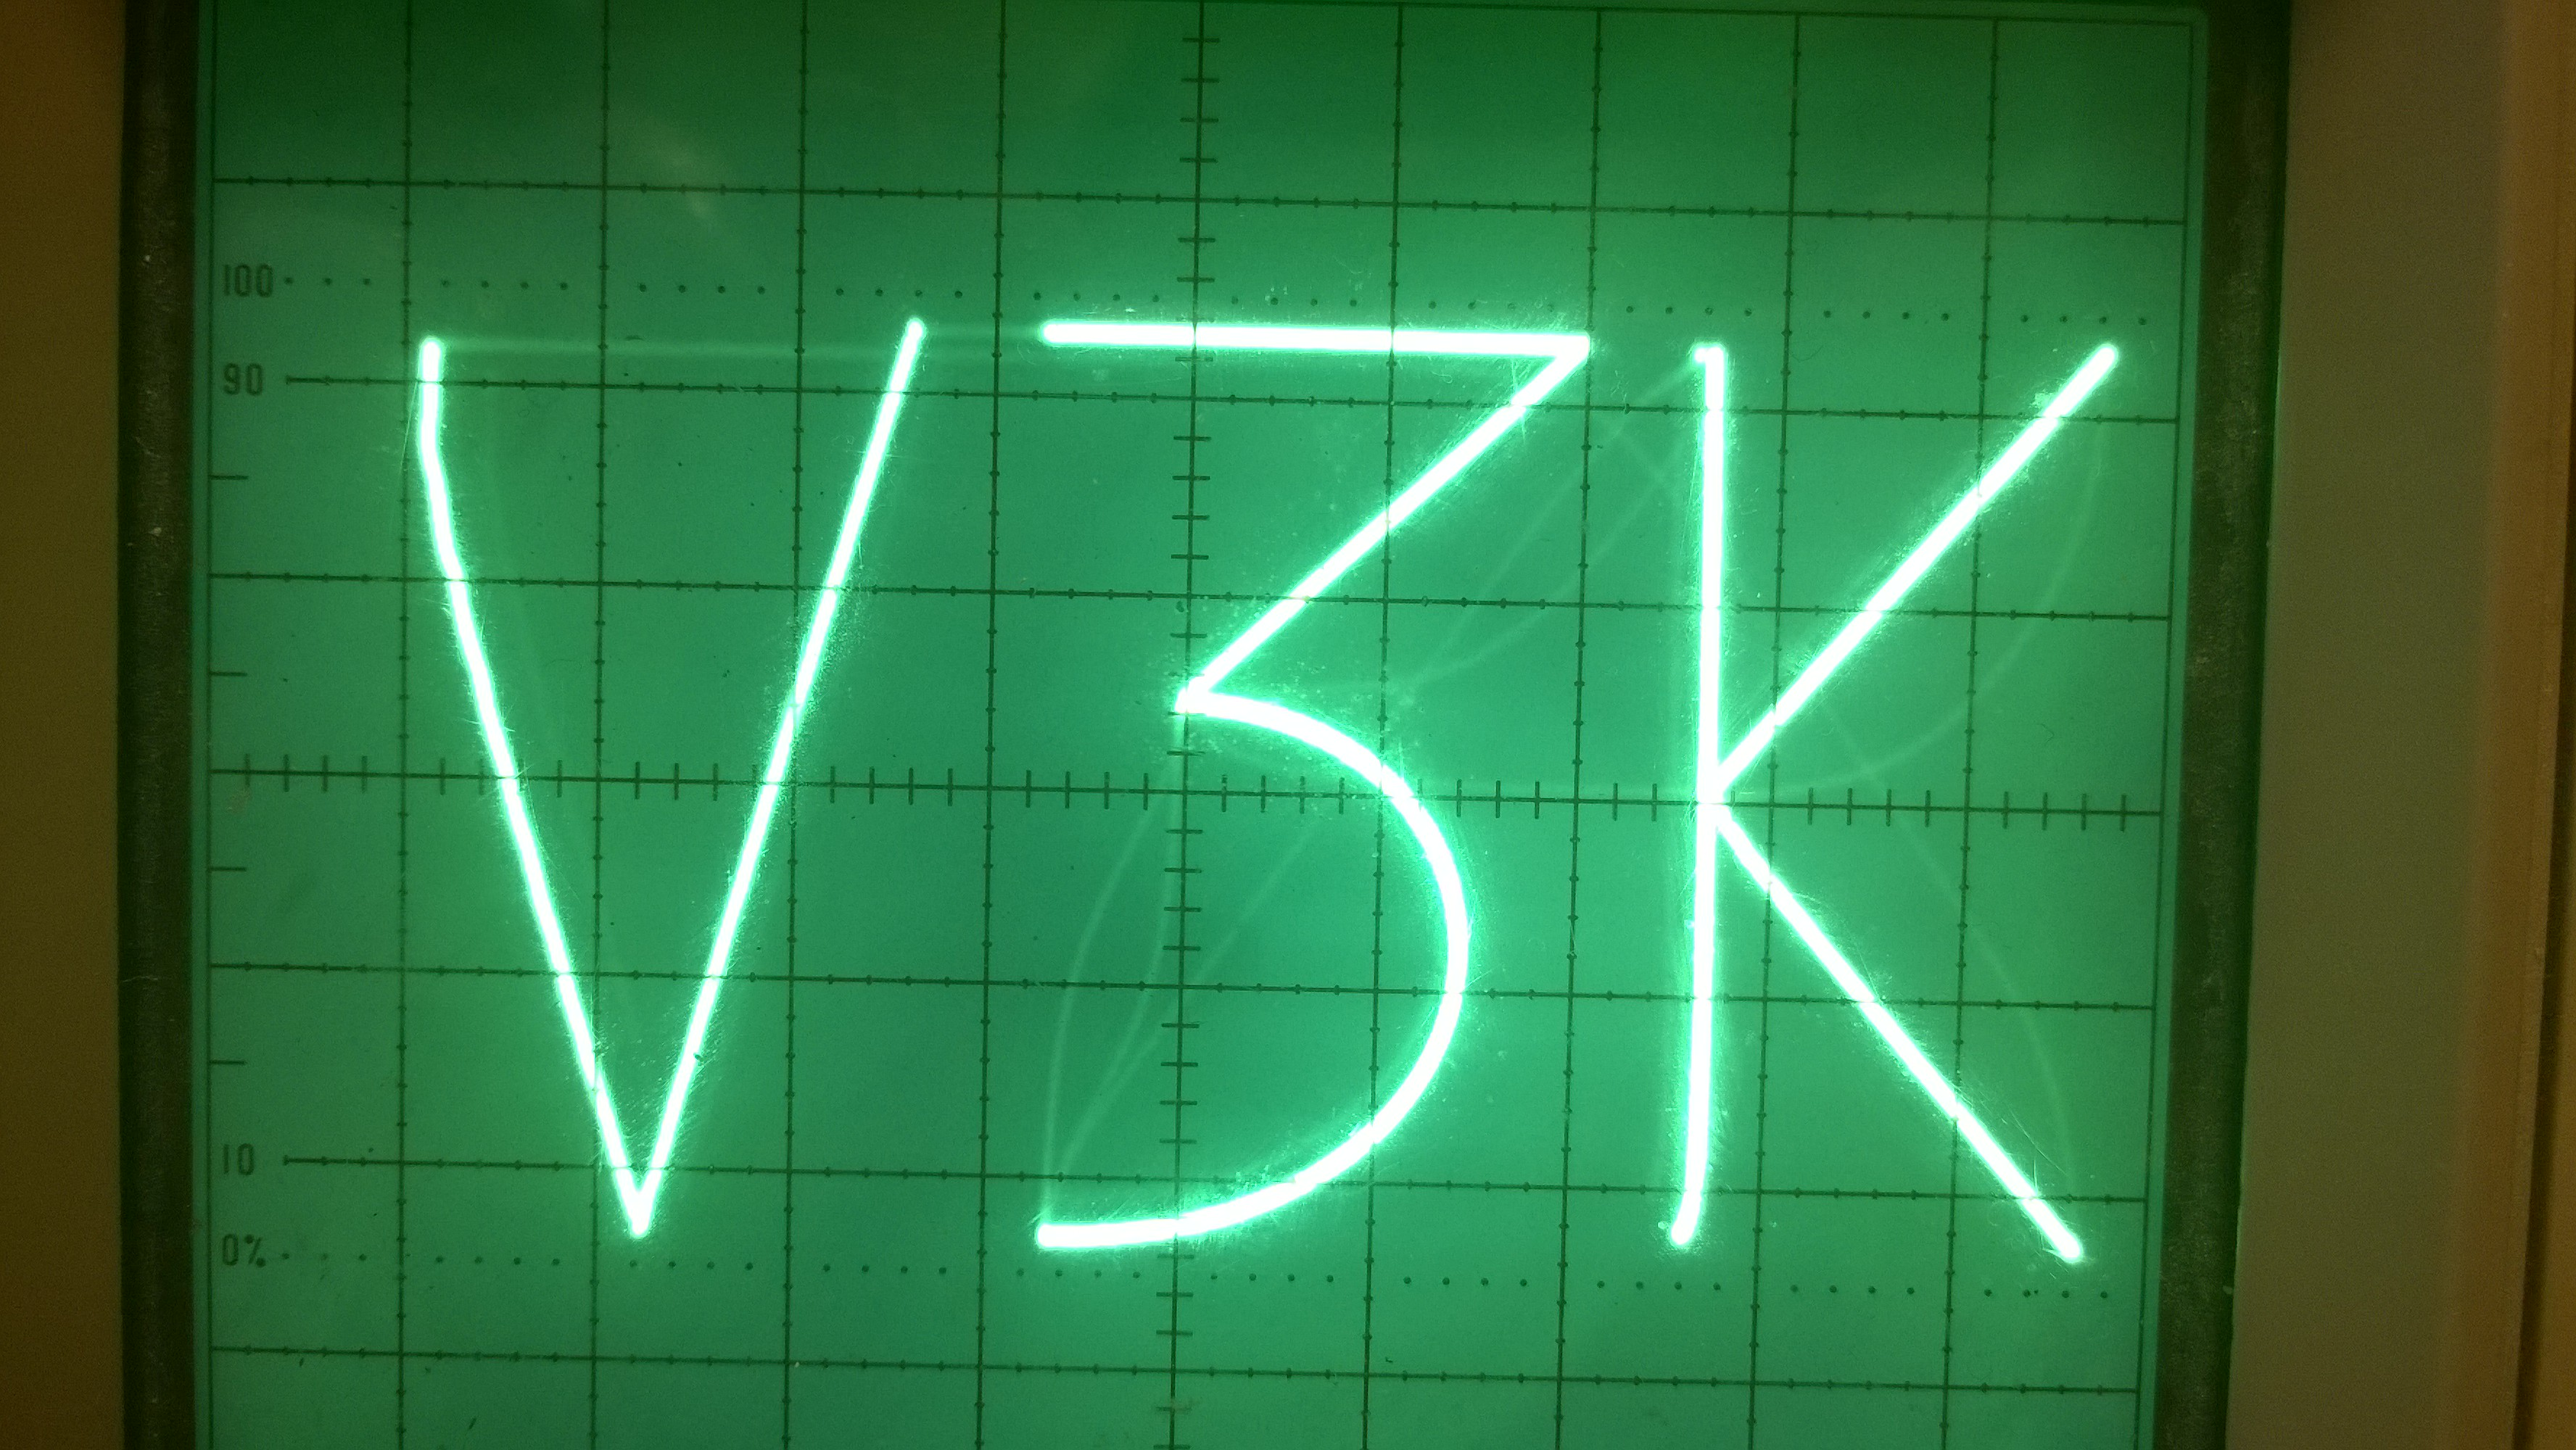
\includegraphics[width=\linewidth]{images/artefacts.jpg}
	    \caption{Drawing V3K with artefacts}
	    \label{fig:artefact}
\end{figure}

Another artefact, also barely visible, is the dots that each primitive is made of.
By zooming in on the oscilloscope this becomes more visible, and can be seen in Figure \ref{fig:artefact-dots}.
The digital nature of \vthreek results in discrete increments when drawing.
The electron ray moves faster than the \gls{dac}s are able to feed it with new data.
As a result, the ray will wait at one spot, until it receives new values.
This results in dotted lines, shown in Figure \ref{fig:dotx4} and \ref{fig:dotx8}

\begin{figure}[h!]
   	\centering
    \begin{subfigure}[b]{\textwidth}
   		\centering
       	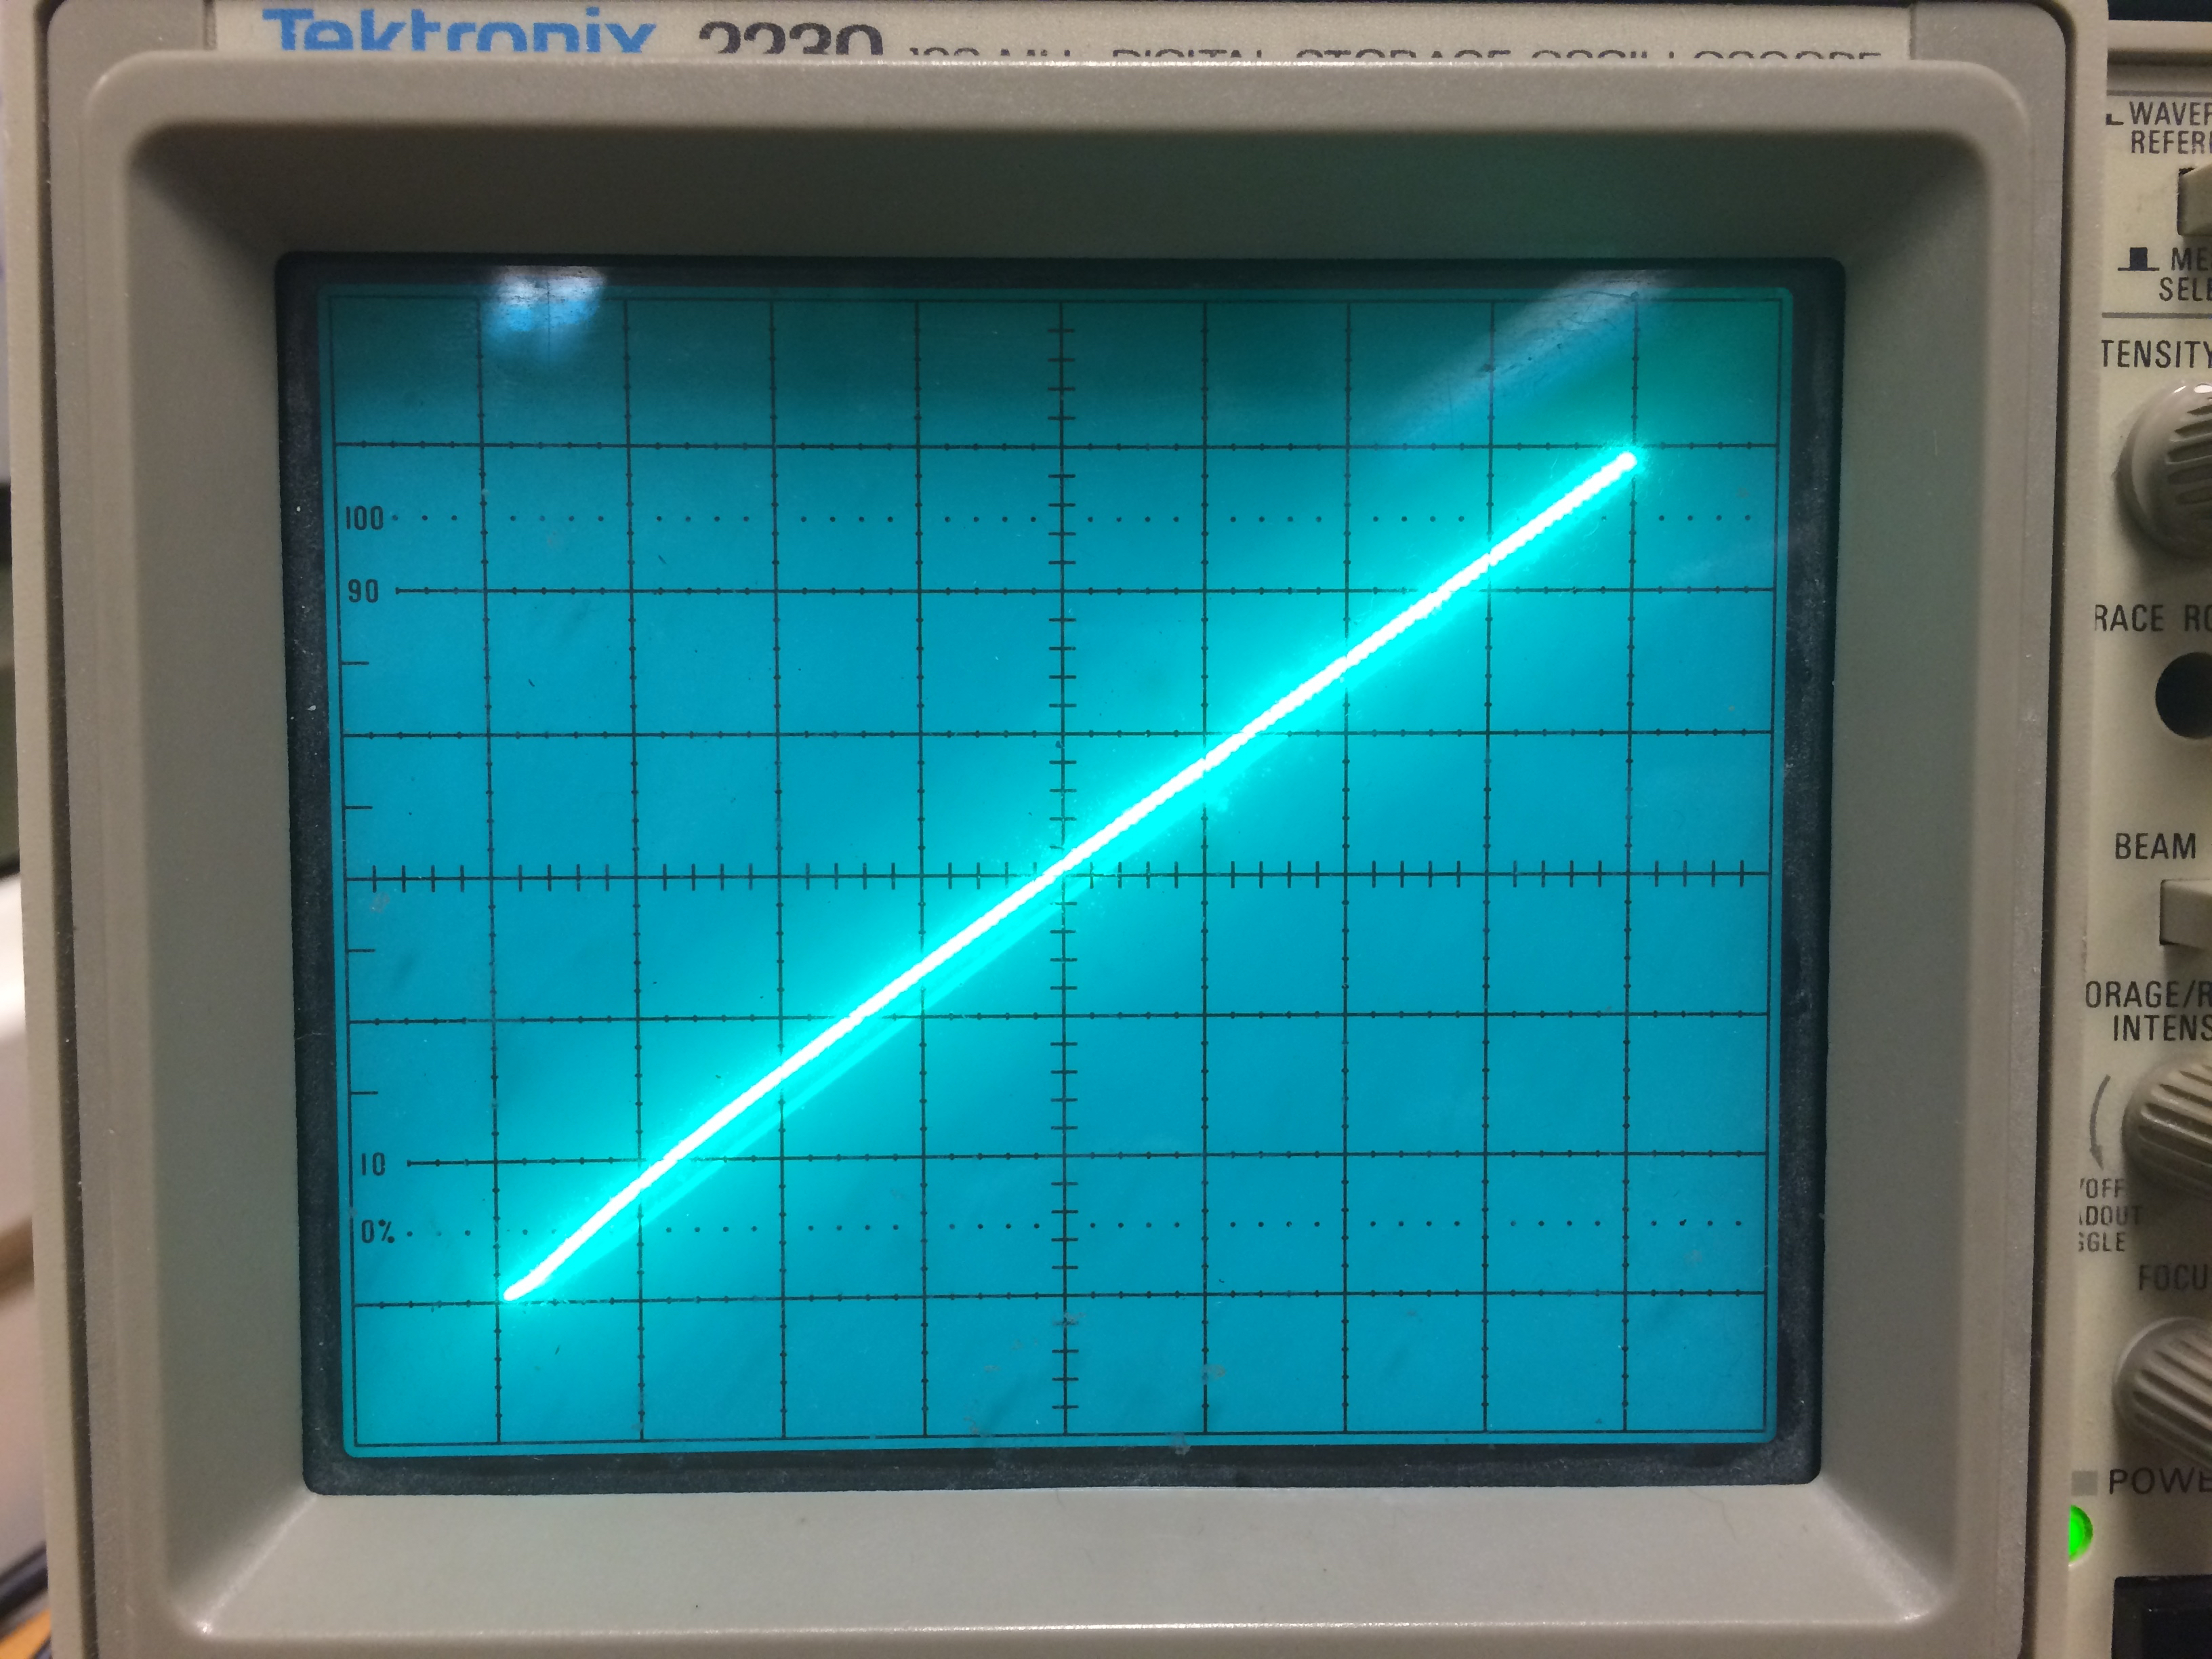
\includegraphics[height=0.4\textheight]{images/dots_x1.jpg}
       	\caption{Dot artefact close to invisible.}
       	\label{fig:dotx1}
    \end{subfigure}
\end{figure}

\begin{figure}[h!]
	\ContinuedFloat
    \begin{subfigure}[b]{\textwidth}
		\centering
        \includegraphics[height=0.4\textheight]{images/dots_x4.jpg}
        \caption{Dot artefact becomes more visible when zoomed in four times.}
        \label{fig:dotx4}
    \end{subfigure}

    \begin{subfigure}[b]{\textwidth}
		\centering
        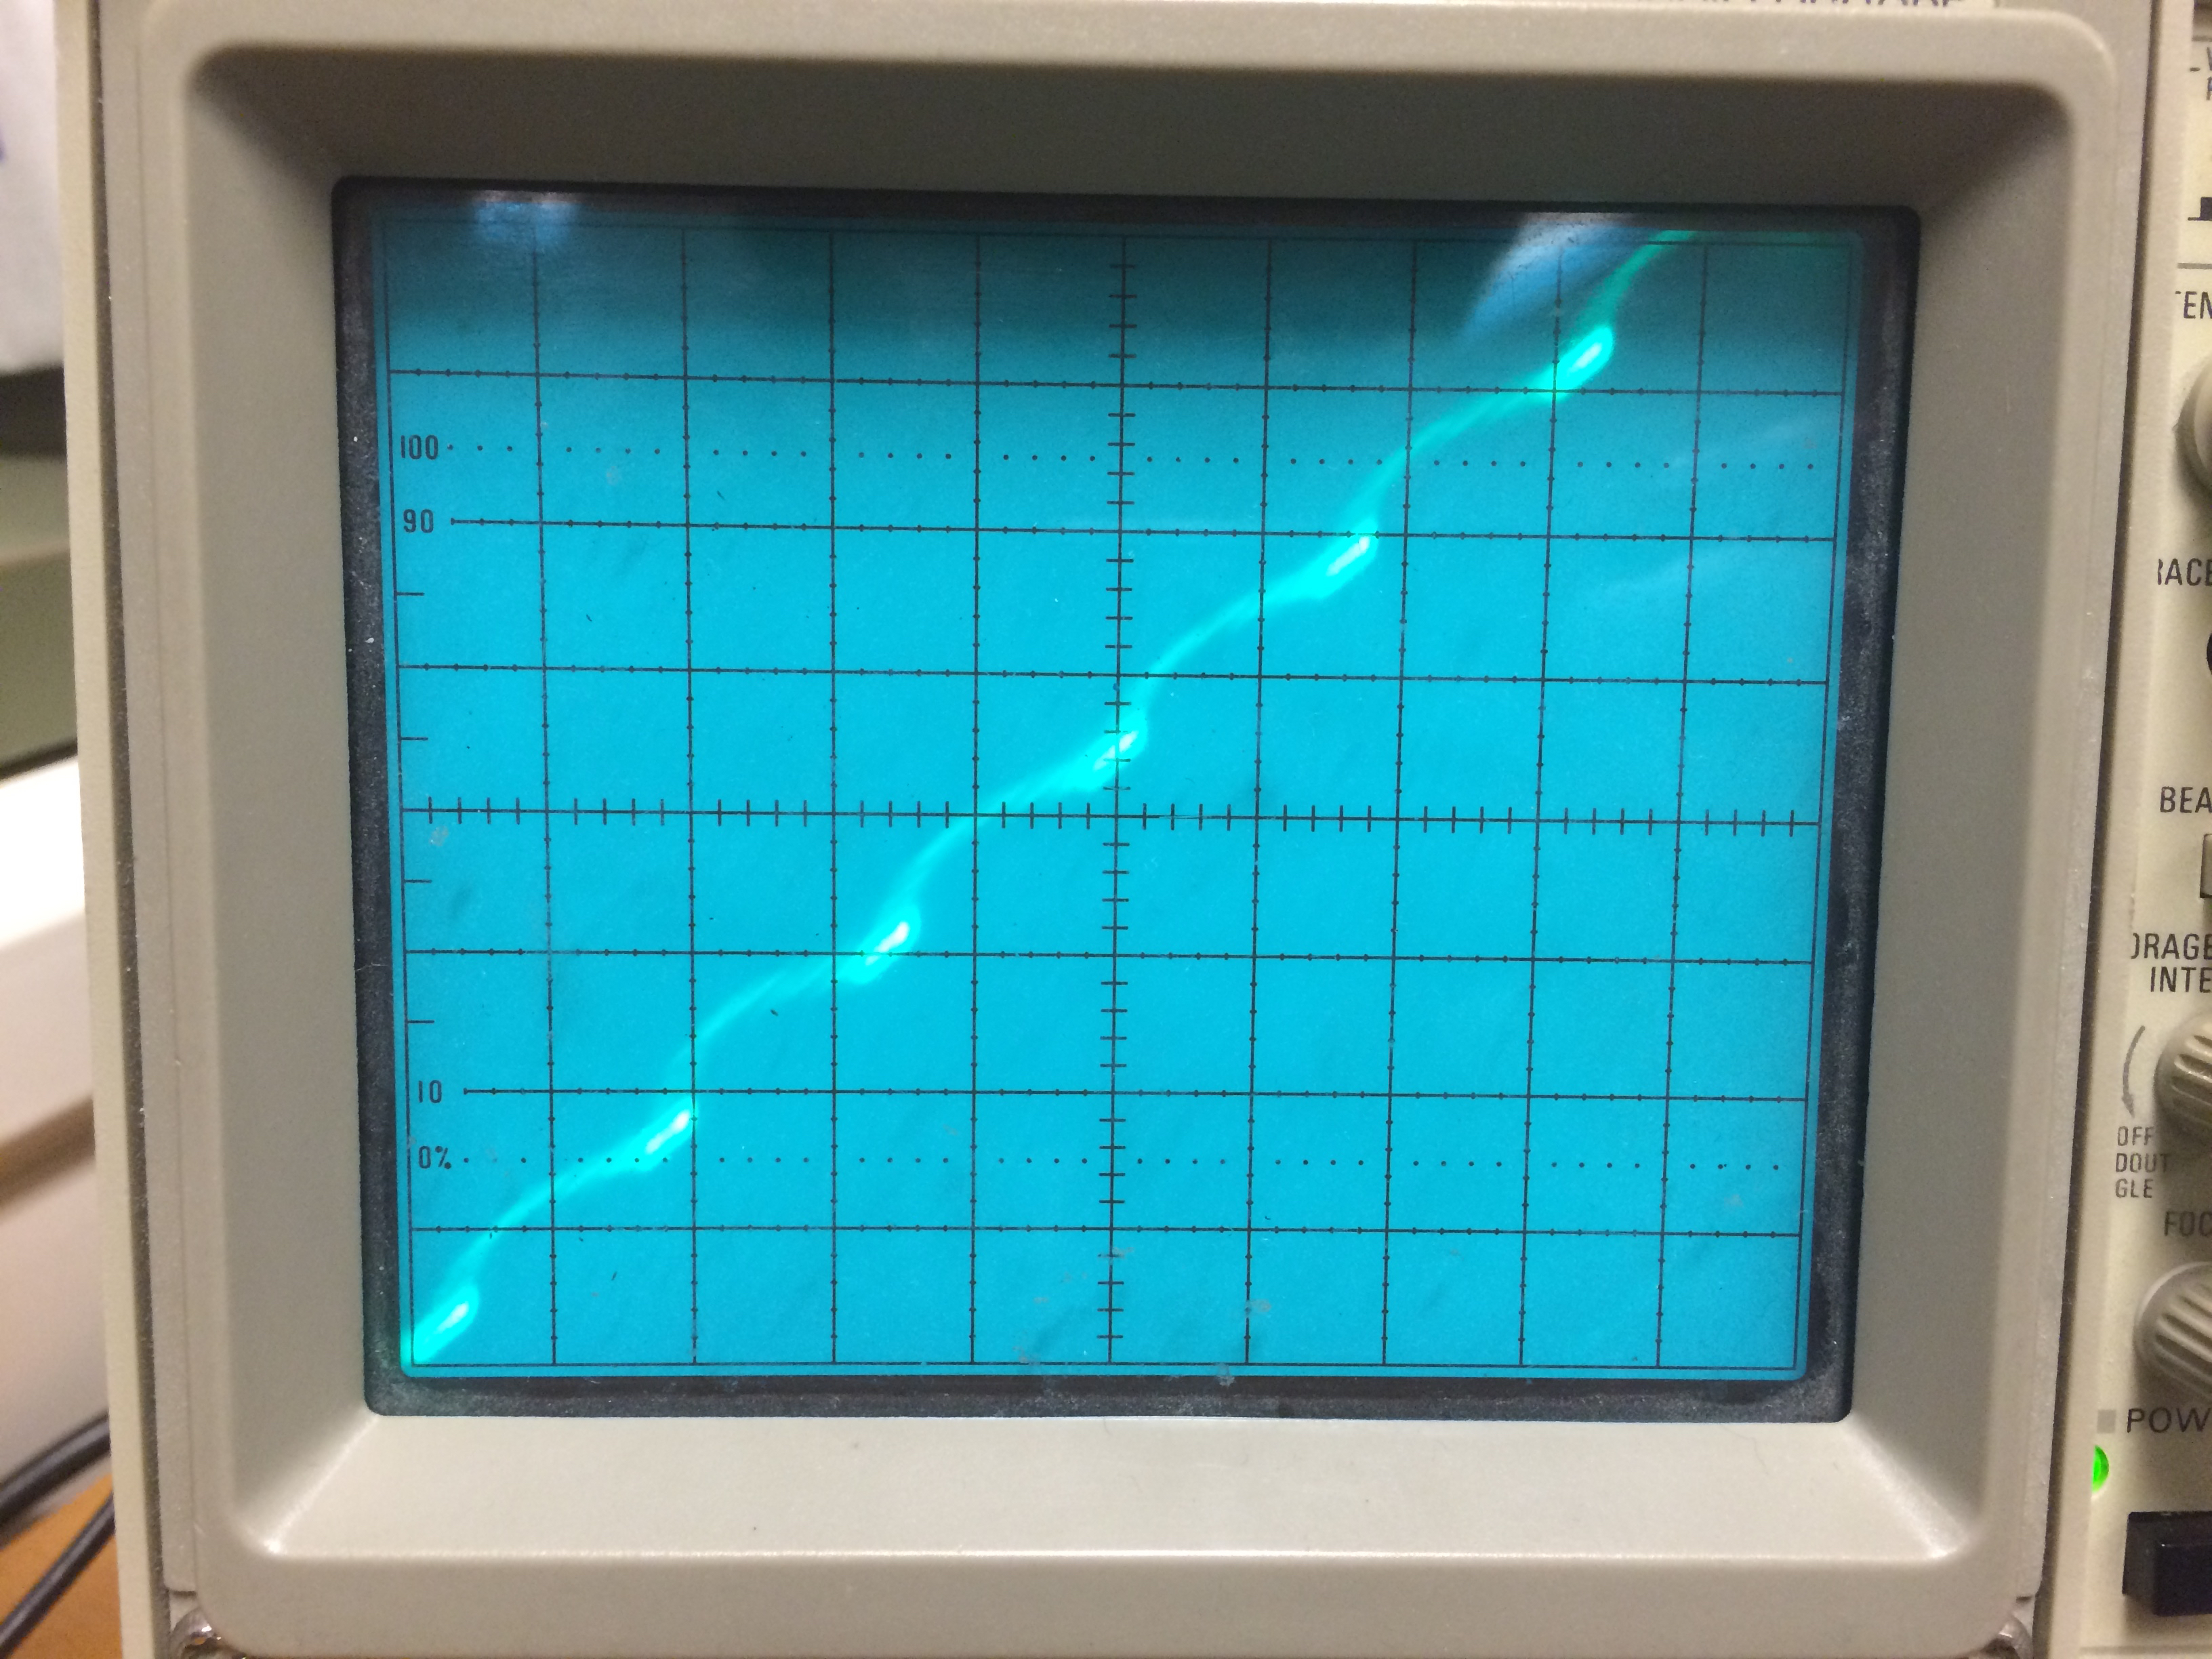
\includegraphics[height=0.4\textheight]{images/dots_x8.jpg}
        \caption{Zooming in eight times, we can also observe that the electron ray do not move in a straight line from point to point.}
        \label{fig:dotx8}
    \end{subfigure}
    \caption{A diagonal line with different levels of zoom}
    \label{fig:artefact-dots}
\end{figure}

\subsection{HDMI}
Rasterisation and \gls{hdmi} were not implemented.
The intention of this part was to demonstrate the difference between vector and raster output in real-time.
However, these parts of the system were no longer prioritized when the analogue counterpart proved to be a reliable source of output.
Moreover, this part was a medium priority requirement, listed in Table \ref{tbl:non_func_req}, and thus not a critical part of \vthreek.

\section{Budget}
In the assignment text, the group was given a budget of 10,000 NOK.
At the end of the project the total cost of materials was about 11,500 NOK (without shipping costs), which is somewhat above the proposed budget for the project.
The full list of material expenses is listed in Appendix \ref{tbl:material-cost}.

\chapter{Discussion}

The group faced some issues during the design process.
This chapter discusses the significant obstacles encountered, and how the group managed to fix or work around them.
Additionaly, possible improvements that were thought about are addressed in the section's end.

\section{PCB Design Errors and Workarounds}
Design errors were discovered shortly after recieving the \gls{pcb} boards.
This section discusses the more serious ones in detail, and how each problem were solved.

\subsection{Routing Problems}
\label{Routing Problems}
Several complications during the routing procedure were encountered.
Most were a product of bad Altium settings, causing some extra time to locate.
The most significant ones are described in detail in the following sections.

\subsubsection{Bad Auto Router Settings}
After auto routing the whole thing the first time, the result contained over 100 still unrouted connections,
which meant that the auto router didn't manage to connect these.

The team discovered that choosing different routing options for the auto router made a big difference.
After making the auto-router focus more on switching layers for every signals,
to avoid complex routing on fewer layers, it managed to route all the connections.
This was achieved by changing routing strategy from \emph{Default 2 Layer Board} to \emph{Default Multi Layer Board} in Altium.

Several auto routing attempts resulted in short-circuits caused by clearance constraint issues, but these were solved by setting the Altium clearance rule to \emph{Different Nets Only}.

\subsubsection{Dead Copper}
Dead copper is parts of the copper on a power plane that's isolated from the rest of the copper on that plane.
This appeared several places on the \gls{pcb}. Normally a minimal problem, but some places a GND via or a 3.3V via was connected to dead copper on the corresponding power plane.
Such issues need to be avoided due to potential heat build-up, so the team repositioned neighboring vias to rejoin the copper area with the rest of the copper plane. The issue and solution are described in figure \ref{fig:Dead copper}.

\begin{figure}[h!]
\centering
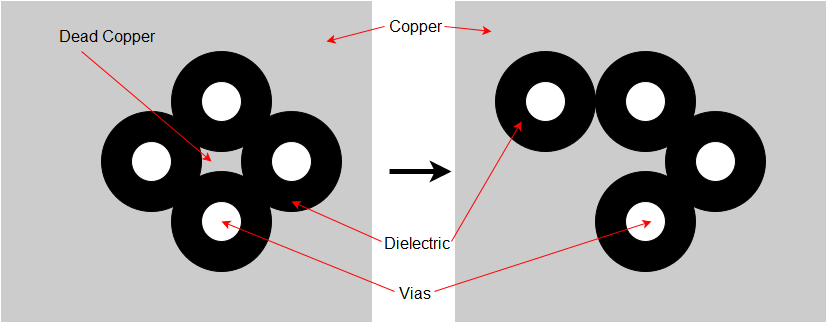
\includegraphics[scale = 0.4]{images/Dead_Copper.png}
\caption{Dead Copper. To the right, dead copper is avoided by moving one via.}
\label{fig:Dead copper}
\end{figure}

\subsection{Possible Routing Improvement}
The auto router caused some wires to make long detours.
Manual routing of some signals could've shortened these distance, but was not critical to the design.
Wires in the same parallell buses should ideally have equal lengths, to ensure all signals in are synchronized.
Some wires in the \gls{ebi} bus, and the bus between the \gls{fpga} and the frame buffer, had varying lengths - potentially create race conditions.
No anomalies were discovered, and the team assumed it was not a problem.
However, modern general purpose computers should be careful to avoid these race conditions \cite{race-conditions}.

\subsection{Bad Soldering}
Some issues arised because of components not being properly soldered onto the \gls{pcb}. Examples are component pins with partial or no contact to the \gls{pcb}, and pins touching several footprint connectors.

\subsubsection{Partially Soldered Voltage Regulator}
It was critical to verify that the power planes worked, as the computer would be dead without power.
Every necessary part that delivered power was soldered on, including power headers and the 3.3 voltage regulator.
External power was run through the power headers.
Measuring different places with a multimeter, anomalies were discovered.
The voltmeter showed only 2.3V, instead of 3.3V.
Further testing revealed that one of the voltage regulator pins hadn't been soldered properly, resulting in a loss of 1V.
Fixing this, the digital \(V_{CC}\) plane contained the correct 3.3V.

\subsection{Incorrect Wiring}
Most \gls{pcb} problems were due to incorrect wiring.
Either signals were having unexpected values, short-circuits had occurred, or other unexpected behaviour.
In the next sections, the most significant wiring issues are addressed and how they were fixed.

\subsubsection{Short-circuits in Buttons}
The group discovered that the buttons were wired wrong, since they caused short-circuits.
The reason was sloppy study of the datasheet, as shown in figure \ref{fig:Button Issue}.
Luckily, this could be remedied by rotating the button 90 degrees, if adjusting the physical connectors to fit the footprint.

\begin{figure}[h!]
\centering
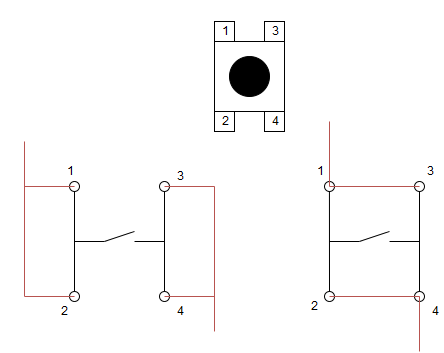
\includegraphics[scale=0.5]{images/Button_Issue.png}
\caption{Top figure shows the button as it looks like on the \gls{pcb}. On the left: Correct wiring according to datasheet. On the right: Incorrect wiring leading to short-circuit}
\label{fig:Button Issue}
\end{figure}

\subsubsection{No Output from Oscillators}
Testing the oscillators, they did not seem to work.
The datasheet for these components clearly stated that connecting the E/D pin to either 'No Connect' or '1' equaled active, so the team did not connect it.
When E/D was connected to \(V_{CC}\), the problem was solved.

\subsubsection{Incorrect Power Supply to Vref and DACs}
The Vref chip was supplied with 3.3V, but should have been supplied with analogue 5V instead.
This could be remedied by cutting on the 3.3V power trace, since the trace is located on the top layer and no other traces are beneath it.
The analogue 5V could then be connected via header from the voltage regulator to the input pin on the Vref chip.
\newline
The DACs were supplied with analogue 5V, but should have been supplied with 3.3V; the analogue 5V should go to the Vref chip instead.
This was solved by switching the two connections.

\subsubsection{Faulty Connected BNCs}
The \gls{bnc} connections were faulty wired.
Each \gls{bnc} had two connections, excluding the socket itself, connected to the \gls{bnc} cable.
One of these would go to ground, while the other would receive the signal destined for the oscilloscope, but these connections was switched.
The group fixed this by running wires to the correct connections.

\subsubsection{FPGA Configuration Issue}
When the \gls{fpga} would complete configuration, it was supposed to set a signal high, which was connected to the \gls{mcu}, saying it was ready. ¨
However, the \gls{mcu} seemed to ignore this signal.
What caused this problem was too hasty study of the manual describing configuration of the \gls{fpga}.
An unnecessary connection to \(V_{CC}\) forced the Done signal into the \gls{mcu} to always be high, even when the \gls{fpga} was not configured.
Since the \(V_{CC}\) connection couldn't be removed, a workaround had to be devised.

By introducing a transistor, and making the signal active low on the \gls{mcu} side, the group managed to make the \gls{mcu} notice when configuration was complete.
The problem and solution is shown in detail in figure \ref{fig:Done Issue}.
This solution was possible because the wire went through the \gls{jtag} header.

\begin{figure}[h!]
\centering
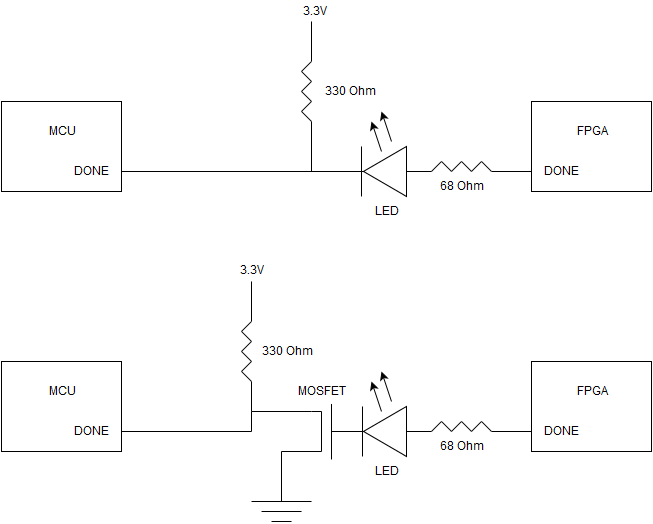
\includegraphics[scale=0.5]{images/Done_Signal_Issue.png}
\caption{Problem and solution of Done signal
         \newline
         Top: Done signal into \gls{mcu} was always logical high
         \newline
         Bottom: Done signal into \gls{mcu} was now active low. The transistor was activated when the configuration was complete, forcing the 3.3V to ground}
\label{fig:Done Issue}
\end{figure}

After further studying of the \gls{fpga} configuration manual \cite[page 42]{fpga-configuration},
it was discovered that the manual was different from what was intended in the group's design,
so there was need for an extra \(V_{CC}\) connection.

\subsubsection{Noise Reduction}
The diode which was intended to reduce noise in the analogue plane, had no noticable effect.
The reason was probably focus on the current leakage, and not noise itself.
The team solved this using a ferrite bead instead of the diode.
A ferrite bead is a component designed to suppress high-frequency noise.

Noise was reduced, but the ferrite bead itself worked also as a resistor, allowing only a small current flow through.
Connecting a resistor with very low resistance (15 Ohm) in parallell with the ferrite bead, current was able to flow freely through this connection.

\subsection{PCB Placement and Footprints}
It would have been beneficial to place the 3.3V voltage regulator closer to the \gls{jtag} debugging port, since the Xilinx \gls{jtag} platform cable required a 3.3V power supply.

The micro \gls{usb} footprint originally contained mounting holes, but were for some reason never drilled during manufacturing.
Luckily, these did not act as connectors, and the team could therefore solder the \gls{usb} receptacle onto the \gls{pcb} like a surface mounted component.

\subsection{Component sizes}
In hindsight, it would have been better to order bigger components.
Since this was a prototype board with mostly hand-soldering, an increase in size would only be beneficial.
Should the project should go into large scale production, the size could have been reduced.


\section{Component Ordering}
The group feels they could've been more thorough with datasheet inspection before finalising component orders.
While waiting for the first delivery, it was discovered that the ordered \gls{led}s were reverse mounted, and not compatible with the \gls{pcb}.
Hence, a new set of \gls{led}s with the correct footprint were ordered.
While this was a cheap component, it could very well have been an important component, resulting in unnecessary delays and waste of money.

Several \gls{dac}s were destroyed, caused by short-circuits during testing.
This resulted in a shortage of \gls{dac}s, which were essential for the design.
For future reference a surplus of fragile components should be ordered.

\section{Oscillator}
To acheive a high clock frequency on the \gls{fpga}, a 100 MHz oscillator was added to the board.
Using it as the main clock signal, the \gls{fpga} was not able to produce correct output.
An oscilloscope was used to measure the oscillator output on a header.
If a hand was placed in close proximity of the board, the oscillator signal was significantly affected.
This problem was solved by using the 48 MHz oscillator instead.

\section{Drawing Artefacts}
\label{discussion:artefacts}
The drawing artefacts explained in Section \ref{results:artefacts} are possible to remove.
If a third input value for intensity were to be added, one could turn the electron beam off when moving the beam between primitives.

The other artefact mentioned, the dotted lines, could be removed by adding analogue circuitry between the \gls{dac} output and the BNC connectors.
It is possible to slew the electron beam from one point to the next, using analogue integration, to archive a smooth transition between points.
An example of such circuitry has been implemented in the 80's in a similar project \cite{vector-graphic-crt}.

If \vthreek were to support an intensity value in addition to x and y, the architecture and \gls{pcb} would require changes.

\section{Improvements}
Further improvements - which ultimately were not implemented due to time constraints or complexity - were discussed by the group and detailed here.

Before any actual coding and soldering, the group spent some time planning the architecture. It was argued that implementing floating point would better conform to the industry standards of vector calculation, and that it would offer more precise calculations.

The auto router caused some wires to make long detours.
More manual routing of signals could've generally shortened these distances.
Wires in the same parallel buses should ideally have equal lengths, to ensure all signals in are synchronized.

The final implementation of the processor is a multi-cycle RISC/MIPS inspired processor.
In this design, one instruction is executed each for second or third clock cycle.
To increase the number of instructions per cycle, the processor could have been pipelined.
Given the time constraint, the group never found the time to implement a pipelined processor.

The processor could also have been made into a multi-core processor, which would further improve the performance. Ultimately, time constraints caused this project to come to a halt.

Interactivity between the user and the graphics could have been implemented, using the included buttons and joystick. A game was discussed as a possible demo, but was deemed to complex and time demanding, given that other parts of the system were more critical to implement.

A toolchain to make it easier for programmers to program on the computer was not prioritised high enough to be done anything with.

The \gls{isa} could have been extended, i.e. with convenient operations that would shorten the program length and solve unintuitive syntax.

\chapter{Conclusion}

\section{Improvements}
The final implementation of the processor, is a multi-cycle mips inspired processor.
In this design one instruction is executed each for second or third cycle.
To increase the number of instructions per cycle, the processor could have been pipelined.
But given the time constraint, the group never found the time to implement a pipelined processor.

\section{Learning Process}
The computer design project gave the group members valuable insight about how to create a computer from start to finish.
A lot of the "magic" behind computer design is removed after completing this project.


% Glossary
\glsaddall
\printglossaries

% Bibliography - edit references.bib and use the \cite command in text
\printbibliography

% Part IV
\part{Appendices}
\begin{appendices}
\chapter{Bill of Materials}
\label{app:bom}
\begin{longtable}{|l|c|}
	\hline
	\textbf{Description} & \textbf{Amount} \\ [0.5ex]
	\hline
	BNC & 2 \\ \hline
	Button & 4 \\ \hline
	Capacitor, 10pF & 2 \\ \hline
	Capacitor, 15pF & 3 \\ \hline
	Capacitor, 10nF & 3 \\ \hline
	Capacitor, 100nF & 20 \\ \hline
	Capacitor, 470nF & 13 \\ \hline
	Capacitor, 1uF & 10 \\ \hline
	Capacitor, 4.7uF & 9 \\ \hline
	Capacitor, 10uF & 2 \\ \hline
	Capacitor, 100uF & 6 \\ \hline
	Diode & 1 \\ \hline
	DAC & 2 \\ \hline
	EFM32GG microcrontoller & 1 \\ \hline
	Flash memory & 1 \\ \hline
	FPGA, Xilinx Spartan 6 & 1 \\ \hline
	HDMI connector & 1 \\ \hline
	Header 2-pin & 10 \\ \hline
	Header 2x2-pin & 4 \\ \hline
	Header 3-pin & 5 \\ \hline
	Header 3x2-pin & 2 \\ \hline
	Header 4x2-pin & 2 \\ \hline
	Header 5x2-pin & 1 \\ \hline
	Header 6x2-pin & 1 \\ \hline
	Header 7x2-pin & 1 \\ \hline
	Header 8x2-pin & 1 \\ \hline
	Header 10x2-pin & 1 \\ \hline
	Header 16x2-pin & 2 \\ \hline
	Header 19x2-pin & 2 \\ \hline
	Joystick & 1 \\ \hline
	LED & 3 \\ \hline
	Micro-USB connector & 1 \\ \hline
	Oscillator 32kHz & 1 \\ \hline
	Oscillator 48MHz & 1 \\ \hline
	Oscillator 100MHz & 1 \\ \hline
	Resistor 18 Ohm & 1 \\ \hline
	Resistor 39 Ohm & 1 \\ \hline
	Resistor 68 Ohm & 1 \\ \hline
	Resistor 330 Ohm & 1 \\ \hline
	Resistor 4.7 kOhm & 2 \\ \hline
	Resistor 10 kOhm & 4 \\ \hline
	SRAM & 2 \\ \hline
	Voltage reference & 1 \\ \hline
	Voltage regulator 1.2V & 1 \\ \hline
	Voltage regulator 3.3V & 1 \\ \hline
	Voltage regulator 5AV & 1 \\
	\hline
	\caption{Bill of materials for a single board}
	\label{tab:bom}
\end{longtable}

\chapter{Material Cost}
TODO: Add table

\chapter{Instruction Set Architecture (ISA)}
\label{app:isa}
//TODO: Include missing instructions, and reorder.
\begin{table}[H]
    \begin{tabular}{|p{2cm}|p{5cm}|p{4cm}|p{3cm}|}
    \hline
    Instruction & Description                          & Syntax                 & Expression                                                 \\ \hline
    nop         & No operation                         & nop                    & ~                                                          \\ \hline
    jmp         & Jump to label                        & jmp label              & ~                                                          \\ \hline
    mov         & Move constant into register          & mov Rd, \#imm16        & Rd = imm16                                                 \\ \hline
    add         & Addition                             & add Rd, Rs, Rt         & Rd = Rs + Rt                                               \\ \hline
    lsl         & Logical shift left                   & lsl Rd, Rs, \#imm16    & Rd = Rs \verb|<<| imm16                                           \\ \hline
    line        & Create line primitive from registers & line Rs, Rt            & (x0, y0) = Rs, (x1, y1) = Rt                               \\ \hline
    bezquad     & Create quadratic Bezier curve        & bezquad Rs, Rt, Ru     & (x0, y0) = Rs, (x1, y1) = Rt, (x2, y2) = Ru                \\ \hline
    bezcube     & Create cubic Bezier curve            & bezcube Rs, Rt, Ru, Rv & (x0, y0) = Rs, (x1, y1) = Rt, (x2, y2) = Ru, (x3, y3) = Rv \\ \hline
    ldr         & Load word                            & ldr Rd, \#addr         & Rd = *addr                                                 \\ \hline
    str         & Store word                           & str Rs, \#imm          & addr = [Rs]                                                \\ \hline
    ldrp        & Load primitive into regiser          & ldrp \#addr            & Pa = *addr                                                 \\ \hline
    strp        & Store primitive to memory            & strp \#imm             & Pa = *imm                                                  \\ \hline
    beq         & Branch on equal                      & beq Rs, Rt, \# imm16   & if Rs == Rt: Pc = Pc + imm                            \\ \hline
    \end{tabular}
    \caption{The complete ISA for the CPU}
\end{table}

\chapter{Tunnel program}
\label{app:tunnel}
\lstinputlisting[language=sh, commentstyle=\color{blue}]{code/tunnel.v3k}

\chapter{Schematics}
\label{app:schematics}

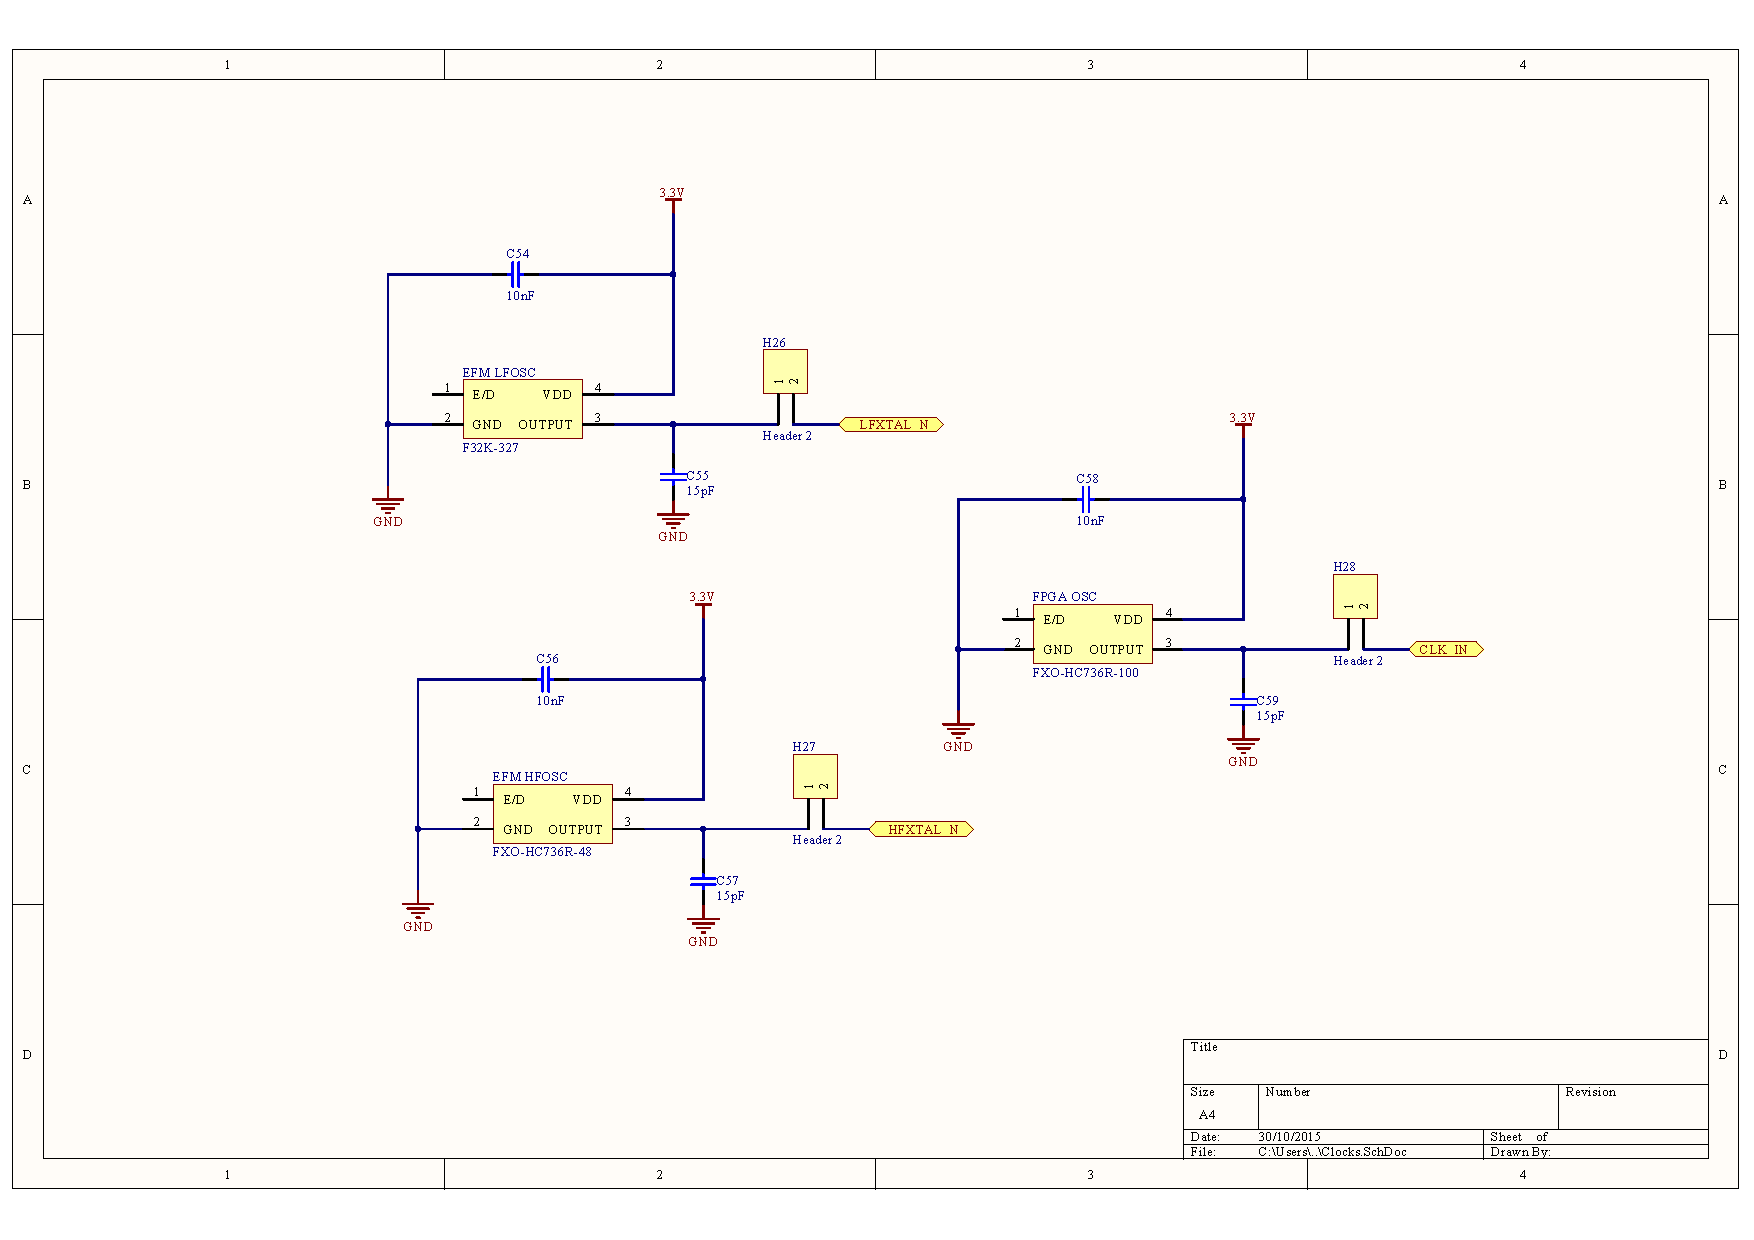
\includepdf[pages=-, landscape=true]{content/appendix/Schematics.pdf}


\end{appendices}

\end{document}
